% ============================================================================
% Appendices. A: farm registry (TODO). B: assumptions register (drafted
% 2026-06-12, post-2024-refit; every value verified against configs, scripts,
% and track READMEs). C: extended tables (TODO). D: reproducibility (short
% draft). E: supplementary figures (TODO). Style: no em dashes.
% ============================================================================

\section{Farm Registry and Data Inventory}\label{app:registry}

The study set is the 31 offshore wind farms of Table~\ref{tab:registry}, sixteen in
the North Sea and fifteen in the Baltic, spanning operational, under-construction,
and planned sites. Each farm's coordinates fix the ERA5 cell its virtual wind farm
samples (Section~\ref{sec:vwf}); capacity and commissioning year are carried for
reference and never enter the capture-value ratio, which is normalised so that rated
capacity cancels. Operational farms, where metered generation exists, are the
validation subset; under-construction and planned sites enter only as price-anchored
panel observations (Section~\ref{sec:fitting}). For recently commissioned farms
the same applies to their pre-commissioning years: Hollandse Kust Zuid came
online in 2023, so its earlier panel rows rest on the validated virtual wind
farm rather than metered output, the method's standard treatment of
not-yet-built capacity. The four German-licensed farms that
stand in Baltic water (zone DE\_LU) are listed under the Baltic by geography but sell into the open German price, so they capture North-Sea-like value.

\begin{table}[!htb]
\centering
\footnotesize
\caption{The 31-farm study registry: market area, location, capacity, commissioning
year, and status. Coordinates are the farm centroid used to select the ERA5 sampling
cell. Sources are developer disclosures, the Crown Estate, and national energy
agencies.}
\label{tab:registry}
\begin{threeparttable}
\begin{tabular}{l l l r r r r l}
\toprule
\textbf{Farm} & \textbf{Country} & \textbf{Zone} & \textbf{Lat} & \textbf{Lon} &
\textbf{MW} & \textbf{Year} & \textbf{Status} \\
\midrule
\multicolumn{8}{l}{\textit{North Sea (16 farms)}} \\
Horns Rev 3              & DK & DK1   & 55.69 & 7.73   & 407   & 2019 & Operational \\
Anholt                   & DK & DK1   & 56.60 & 11.21  & 400   & 2013 & Operational \\
Borssele 1-2             & NL & NL    & 51.70 & 3.02   & 752   & 2020 & Operational \\
Borssele 3-4             & NL & NL    & 51.70 & 2.95   & 731   & 2020 & Operational \\
Hollandse Kust Zuid      & NL & NL    & 52.30 & 4.20   & 1,525 & 2023 & Operational \\
Gemini                   & NL & NL    & 54.04 & 5.97   & 600   & 2017 & Operational \\
Borkum Riffgrund 2       & DE & DE\_LU & 53.97 & 6.55  & 450   & 2019 & Operational \\
Veja Mate                & DE & DE\_LU & 54.31 & 5.86  & 402   & 2017 & Operational \\
Hornsea 1                & GB & GB    & 53.88 & 1.79   & 1,218 & 2019 & Operational \\
Hornsea 2                & GB & GB    & 53.95 & 1.90   & 1,320 & 2022 & Operational \\
C-Power                  & BE & BE    & 51.55 & 2.93   & 325   & 2013 & Operational \\
Norther                  & BE & BE    & 51.50 & 2.95   & 370   & 2019 & Operational \\
Saint-Brieuc             & FR & FR    & 48.82 & $-2.55$ & 496  & 2024 & Operational \\
Dogger Bank A            & GB & GB    & 54.75 & 1.85   & 1,200 & 2025 & Under constr. \\
Princess Elisabeth Zone  & BE & BE    & 51.50 & 2.60   & 3,500 & 2030 & Planned \\
North Sea Energy Island  & DK & DK1   & 56.20 & 7.50   & 3,000 & 2033 & Planned \\
\addlinespace
\multicolumn{8}{l}{\textit{Baltic (15 farms)}} \\
Rodsand 1 (Nysted)       & DK & DK2   & 54.55 & 11.71  & 165   & 2003 & Operational \\
Rodsand 2                & DK & DK2   & 54.55 & 11.80  & 207   & 2010 & Operational \\
Kriegers Flak DK         & DK & DK2   & 54.97 & 12.90  & 605   & 2021 & Operational \\
Wikinger                 & DE & DE\_LU & 54.83 & 14.07 & 350   & 2017 & Operational \\
Arkona                   & DE & DE\_LU & 54.78 & 14.12 & 385   & 2019 & Operational \\
Baltic 2                 & DE & DE\_LU & 54.99 & 13.16 & 288   & 2015 & Operational \\
Baltic Eagle             & DE & DE\_LU & 54.79 & 13.92 & 476   & 2024 & Operational \\
Lillgrund                & SE & SE\_4 & 55.51 & 12.78  & 110   & 2007 & Operational \\
Bornholm Energy Island   & DK & DK2   & 55.10 & 14.60  & 3,000 & 2032 & Planned \\
Saare-Liiv               & EE & EE    & 58.30 & 22.50  & 3,000 & 2035 & Planned\tnote{a} \\
Liivi Bay                & LV & LV    & 57.80 & 23.50  & 1,000 & 2030 & Planned \\
Klaipeda offshore        & LT & LT    & 55.80 & 20.60  & 1,400 & 2030 & Planned \\
Baltic Power             & PL & PL    & 55.00 & 17.40  & 1,140 & 2026 & Under constr. \\
Baltyk II / III          & PL & PL    & 55.05 & 17.20  & 1,440 & 2027 & Planned \\
FEW Baltic II / Olhava   & FI & FI    & 64.80 & 24.50  & 1,280 & 2030 & Planned \\
\bottomrule
\end{tabular}
\begin{tablenotes}\footnotesize
\item[a] Saare-Liiv falls on a coastal ERA5 cell and is flagged accordingly.
\item Data coverage: Dutch renewable generation is rescaled to physical capacity
factors (documented ENTSO-E under-reporting); British day-ahead prices end with
Brexit, so the three British farms contribute panel data only through 2020.
\end{tablenotes}
\end{threeparttable}
\end{table}

\section{Assumptions Register}\label{app:assumptions}

Every modelling choice that shapes a number in this thesis is listed here
with its value, its source, and where its influence is tested or bounded.
Items marked (L) reappear in the consolidated limitations of Chapter 5.

\subsection*{B.1 Shared data and definitions}

\begin{enumerate}
    \item \textbf{One capture-value definition.} Generation-weighted price
    over time-mean zone price, on common hours only; zone price is the
    unweighted mean over the zone's network nodes; Denmark splits at
    11$^{\circ}$E into DK1/DK2. Used identically by every component
    (Section~\ref{sec:currency}).
    \item \textbf{Basin membership is geographic.} A farm belongs to the sea
    its foundations stand in; DK2 and SE4 are Baltic-facing although their
    markets sit in the Nordic synchronous area
    (Section~\ref{sec:farm_data}). Corroborated by weather-only clustering
    (Section~\ref{sec:weather_agrees}).
    \item \textbf{ENTSO-E Transparency is the single market-data source}
    (2017 to 2024): prices for 22 zones, load, generation by type, flows,
    capacities. Dutch renewable generation is rescaled to physical capacity
    factors (documented under-reporting); British day-ahead prices end with
    Brexit, so GB farms contribute no farm-months after 2020. (L)
    \item \textbf{ERA5 is the weather truth} (regression: nearest
    0.25$^{\circ}$ cell via Open-Meteo; system model: 0.3$^{\circ}$ yearly
    cutouts via atlite). Its offshore wind-speed bias is not corrected
    explicitly; the Hayes power-curve shift absorbs it, and the end result
    is validated against metered generation (median hourly correlation
    0.88, monthly 0.95, fifteen zone-years).
    \item \textbf{TYNDP 2024 is the scenario authority} for capacities,
    demand, and fuel and carbon prices. The parse covers renewables only;
    the corrections of Table~\ref{tab:corrections} repair the documented
    consequences. (L)
\end{enumerate}

\subsection*{B.2 The system model}

\begin{enumerate}\setcounter{enumi}{5}
    \item \textbf{Scope.} Fourteen countries, 30 clusters with focus
    weights on offshore-heavy markets; Sweden and Norway remain coarse
    (three clusters), so SE is reported with an all-Sweden caveat and NO is
    excluded from headline aggregates alongside GB. (L)
    \item \textbf{Resolution.} Full hourly year (8,760 snapshots; the
    framework drops the 2024 leap day by convention).
    \item \textbf{Frozen transmission} (\texttt{transmission\_limit: v1.0}):
    line and link capacities fixed at today's volume, the conservative
    bound; the optimistic bound is computed explicitly (optimal expansion
    moves clean 2040 scenarios $+0.04$ to $+0.06$, stressed ones $+0.18$ to
    $+0.19$).
    \item \textbf{Year-correct fleets.} Conventional plants filtered by
    commissioning and retirement dates; renewable capacities topped up to
    the run year's national statistics (IRENASTAT via powerplantmatching).
    \item \textbf{Fuel-price overrides} (annual means): 2023 gas
    41.0~\euro/MWh$_{th}$, coal 16.0, lignite 5.5, oil 75.0; 2024 gas 34.7,
    coal 14.0, lignite 5.5, oil 74.0; 2019 uses the 2020 technology-cost
    defaults. Sources: TTF and EUA from the project's monthly series, coal
    from ARA annual means, oil from Brent.
    \item \textbf{Carbon prices}: 25 / 84 / 67~\euro/tCO$_2$ for 2019 /
    2023 / 2024 (EUA annual means), applied through emission pricing.
    \item \textbf{Perfect competition, perfect foresight, linear
    dispatch.} No unit commitment, start-up costs, minimum loads, must-run
    district-heating CHP, or strategic bidding. Consequence: shadow prices
    are too flat in windy hours in small congested zones. This is not left
    as an assumption: it is measured (DK2 bias $+0.143$ in 2023, $+0.141$
    in 2024), explained by the hybrid decomposition, and corrected with
    propagated uncertainty (Section~\ref{sec:bias_method}). (L)
    \item \textbf{Interconnectors are fully available every hour} (no TSO
    de-rating or reservations). Same direction and same treatment as the
    previous item: absorbed into the measured, corrected bias. (L)
    \item \textbf{Scarcity ladder} (correction F): demand response sized at
    5\,\% of each node's peak load offered at 400~\euro/MWh; unserved
    energy at the 4,000~\euro/MWh day-ahead cap; residual unserved energy
    below 0.05\,\% of demand, reported per scenario
    (Section~\ref{sec:scarcity_method}).
    \item \textbf{Scenario corrections A to F} as enumerated in
    Table~\ref{tab:corrections}, including the Danish offshore split
    (65/35 in 2030 to 60/40 by 2040), offshore caps (DK 50, FI 25, SE 35~GW), and
    Poland's announced 3.9~GW of nuclear by 2040.
    \item \textbf{Demand trajectories}: scenario demand is rebased from
    crisis-2023 to 2019 before TYNDP growth; the two countries missing from the scenario tables receive documented growth
fallbacks. All scenario
    horizons are solved on 2023 weather and hourly load shapes, so the only thing that changes across scenarios is the buildout. (L)
    \item \textbf{Hydrogen floor} (correction D): a parametric stand-in
    for sector coupling, with per-country electrolysers, fixed hydrogen
    demand, and a priced import backstop near 35 to 42~\euro/MWh; halving and
    raising its demand by 50\,\% moves the 2040 Baltic capture value by at most
    0.013, and by under 0.01 in the clean DE and GA scenarios
    (Appendix~\ref{app:robustness}). (L)
    \item \textbf{Solver parity.} Gurobi barrier without crossover,
    identical tolerances, for every baseline and every scenario, because
    the bias correction is fitted on interior-point duals and must be
    applied to prices formed the same way.
    \item \textbf{Bias correction.} Linear in the model's own offshore
    penetration; fourteen of fifteen validation points (Netherlands 2019
    excluded as low-confidence observation); clamped at penetration 0.50;
    corrected values floored at zero. The penetration slope is anchored on DK2,
    the only validation zone above 31\,\% penetration: leave-one-zone-out
    collapses it from 0.233 to 0.045 with an interval crossing zero
    (Appendix~\ref{app:robustness}), so the correction is reported as a refinement of the uncorrected system model, which remains the
    source of the result. (L)
    \item \textbf{Gas-price grid}: 15 to 120~\euro/MWh$_{th}$ across three
    buildouts; exposure slopes computed over every offshore zone, with
    basin aggregates excluding GB and NO.
    \item \textbf{Sector-coupled variant}: PyPSA-Eur's sector
    configuration at twelve-hour resolution, thirty clusters, 2019 weather,
    overnight 2040, frozen grid, with heating, hydrogen, storage and
    electric transport co-optimised; country totals pinned to the TYNDP
    2040 fleet (Belgium capped at its 4.9~GW sea-space potential); the
    electricity-only control is identical in every setting. The weather
    cutout spans 47$^{\circ}$N northward, truncating southern France
    identically in both arms. (L)
    \item \textbf{Surrogate emulator}: eight inputs; fifty Latin-hypercube
    training solves at three-hour resolution (full-hourly equivalence
    checked: mean absolute capture-value difference 0.024, up to 0.147
    only at the extreme 139-GW corner); validation by held-out whole
    scenarios; the Baltic correction parsed from the canonical fit. (L)
\end{enumerate}

\subsection*{B.3 The regression model}

\begin{enumerate}\setcounter{enumi}{21}
    \item \textbf{Virtual wind farm}: logarithmic extrapolation from the
    10~m and 100~m ERA5 levels to the 150~m hub height of the IEA 15~MW
    reference turbine \cite{Gaertner2020}, whose power curve enters as a
    hand-keyed table of the published values interpolated on a
    0.25~m\,s$^{-1}$ grid (cut-in 3, rated 10.59, cut-out 25~m\,s$^{-1}$);
    Hayes adjustments $\sigma = 1.17$~m\,s$^{-1}$ and
    $w_0 = 0.71$~m\,s$^{-1}$ (calibrated on 57 metered European farms),
    applied as a Gaussian convolution of the curve followed by a rightward
    shift; output hard-zeroed outside the 3 to 25~m\,s$^{-1}$ operating
    envelope after smoothing, since the convolution otherwise leaks output
    into storm and calm hours. The archived eight-year panel predates this
    re-zero; hours outside the envelope are rare enough to bound its effect
    below half a percent of capture value; the released code applies the re-zero.
    Farms closer than one reanalysis cell share identical output, so
    near-neighbour pairs are excluded from synchronicity comparisons.
    \item \textbf{Monthly capture value} requires at least 500 overlapping
    farm-price hours; capacity factors are normalised, so rated capacity
    cancels in the ratio.
    \item \textbf{Training set}: the bidding-zone market panel, every site
    with observed prices over 2017 to 2024 (all 2,706 zone-months across 31
    sites). The operational farms are the validation subset, the only sites
    where generation can be checked against metered output. (L: metered
    offshore exists only in DK2 and SE4, so the enclosed-Baltic price-only
    zones are anchored on observed prices and a validated wind profile, since no local
    metered generation exists.)
    \item \textbf{Market-area resolution}: features computed at bidding-zone
    level where zone-resolved series exist (DK1, DK2, SE4), country level
    elsewhere, recorded per row. (L)
    \item \textbf{Flexibility index numerator}: openly reported pumped
    hydro plus battery capacity where ENTSO-E reports it, a documented
    substitution for the predecessor's proprietary battery and
    demand-response data. (L)
    \item \textbf{Interconnection index}: realised utilisation, the mean
    absolute cross-border flow over each external border's capacity (proxied
    by its yearly maximum flow), summed across borders. The predecessors'
    neighbour-synchronicity discount is dropped on evidence
    (Section~\ref{sec:features}); static within each year, blind to
    hour-by-hour congestion. (L)
    \item \textbf{Fuel features}: monthly TTF gas and EU ETS carbon
    averages.
    \item \textbf{Collinearity}: variance inflation factors on the 2,706-row
    panel peak at 2.16 (carbon), far below the conventional alarm level of
    five; feature 7 sits at 1.21.
    \item \textbf{No hyperparameter search}; fixed settings for all five
    algorithm families: gradient boosting with 400 trees of depth 4 at
    learning rate 0.05, random forest with 300 trees of depth 8, and
    support-vector, polynomial and linear regression at library defaults
    (library versions in Appendix~\ref{app:repro}); the untuned predecessor
    result is the comparator.
    \item \textbf{2022 retained} in training; an ex-2022 variant is
    reported alongside, mirroring the predecessor's crisis treatment.
    \item \textbf{Projection feature choices}: pattern correlations held
    at the site's recent monthly shape; penetration scaled by TYNDP
    renewable growth over demand growth, anchored on the observed present;
    interconnection held at its recent value (no future border capacities exist in the scenario tables, a mildly
optimistic simplification, with a
    conservative-bound sensitivity that lets utilisation decline as
    renewables grow); flexibility grows with the scenario battery fleet. All
    guarded by the strict all-features range check, the joint convex-hull
    support test, and the carbon-clamp sensitivity. (L)
\end{enumerate}

\subsection*{B.4 The comparison with observation}

\begin{enumerate}\setcounter{enumi}{32}
    \item \textbf{Independence of the three-way comparison's columns}: the regression
    column is out-of-fold (the model never trained on the zone's farms);
    the system column uses no market price data; observation arbitrates.
    \item \textbf{Hybrid decomposition}: model generation priced at
    observed prices isolates whether an error lives in the wind or in the
    price structure.
    \item \textbf{Aggregation difference}: the regression's zone capture
    value is a simple mean over farm-months while the system model's
    is energy-weighted; a small, documented difference.
    \item \textbf{The DK2-analogue premise}: the system model's bias
    transfers along the penetration axis from validated zones to projected
    ones. This is tested directly: the bias replicates across 2023 and 2024,
    the fit's slope interval excludes zero, and no single zone-year moves
    the leave-one-out range.
\end{enumerate}

\subsection*{B.5 The analytical equation in full}

Because an additive split cannot express the shape of the mechanism,
Jacquet's analytical equation is refit as well \cite{Jacquet2024}. It is not a
black box, nor an arbitrary curve: it is a parametric form assembled, term by term,
from the cannibalisation mechanism of Section~\ref{sec:value_problem}. A farm
that sold at random hours would earn the average price, a capture value of one;
cannibalisation is what subtracts from that one. The equation writes that
subtraction as two physical channels, a cannibalisation term and a fuel-price
distortion term, so that every constant in it is a named lever on a specific
channel rather than a free coefficient fit for its own sake:
%
\begin{equation}
    \mathrm{CV} \;=\; 1
    \;-\; B\,\frac{M_{\mathrm{WF}}}{M_{\mathrm{BZN}}}\,S
    \;-\; C\,M_{\mathrm{WF}}\,
    \bigl(0.202\,p_{\mathrm{CO_2}} + p_{\mathrm{gas}}\bigr)^{\gamma}.
\end{equation}
%
where $S$ is the renewable market share and $p_{\mathrm{gas}}$,
$p_{\mathrm{CO_2}}$ the monthly fuel and carbon prices, folded together by the
0.202~tCO$_2$/MWh emission intensity of gas. The first term is cannibalisation:
the wind-pattern penalty $M_{\mathrm{WF}} = \mathrm{sign}(\rho_{\mathrm{VRE}} -
\rho_{\mathrm{load}})\,|\rho_{\mathrm{VRE}} - \rho_{\mathrm{load}}|^{\alpha}$
grows when a farm tracks the system's renewables more than its demand. It is
scaled by penetration $S$ and divided by the buffering term
$M_{\mathrm{BZN}} = (I_{\mathrm{int}} + I_{\mathrm{flex}})^{\delta}$, in which
interconnection and flexibility absorb it. The second term is fuel-price
distortion.

The constants carry the mechanism. The pattern-penalty exponent $\alpha$ sets how
sharply the penalty escalates as a farm's wind aligns with the system's. The
\textbf{cannibalisation scale} $B$ is its overall strength: it multiplies the whole
crowding-times-penetration term, so a larger $B$ means a given amount of crowding
and penetration erodes more value. The \textbf{buffering exponent} $\delta$ governs how strongly interconnection and flexibility reduce that erosion: the penalty is
divided by $(I_{\mathrm{int}} + I_{\mathrm{flex}})^{\delta}$, so a larger $\delta$
makes interconnection and flexibility more protective per unit of capacity. $C$
scales the fuel-price distortion term and $\gamma$ sets its curvature. They are fit
by bounded least squares, separately for the pooled data, the North Sea, and the
Baltic, with a 200-resample farm-block bootstrap for intervals. Because the
constants trade off inside shared terms, no single one is read in isolation; the
basins are compared by the quantity they jointly produce, the implied slope of
capture value against penetration, at common reference conditions.

\subsection*{B.6 The spatial cost model in full}

Offshore capital cost rises with both: deeper water
demands heavier foundations, and farther sites demand longer export cables.
Writing $c_0$ for the turbine-and-array base, $\phi(d)$ for the foundation, and a
linear export term beyond a near-shore allowance $\ell_0$,
%
\begin{equation}
  \mathrm{CAPEX}(d,\ell) \;=\; c_0 \;+\; \phi(d) \;+\; \gamma\,\max(\ell-\ell_0,\,0),
  \qquad
  \phi(d) =
  \begin{cases}
    a_{f}\,\max(d-d_0,0), & d \le d_1,\\[2pt]
    a_{f}(d_1-d_0) + c_{\mathrm{fl}} + a_{\mathrm{fl}}(d-d_1), & d > d_1,
  \end{cases}
  \label{eq:costmodel}
\end{equation}
%
with $c_0 = 1.85$~M\euro/MW, $d_0 = 25$~m, $d_1 = 60$~m, fixed-bottom slope
$a_{f} = 12$~k\euro/MW/m, a floating premium $c_{\mathrm{fl}} = 1.0$~M\euro/MW
appearing past $d_1$, floating slope $a_{\mathrm{fl}} = 6$~k\euro/MW/m, export term
$\gamma = 10$~k\euro/MW/km, and $\ell_0 = 25$~km. The piecewise jump at $d_1$ is
the transition from fixed-bottom to floating foundations. Levels are anchored to
the offshore cost database that ships with PyPSA-Eur and to IRENA's 2024 cost
review \cite{Horsch2018, IRENA2025Costs}. Capital is annualised at a capital
recovery factor $\mathrm{CRF} = w(1+w)^n/[(1+w)^n-1]$ with a weighted-average cost
of capital $w = 7\%$ over an economic life $n$ of 27 to 30 years, technology
learning enters through a factor $\lambda(y)$ normalised to unity in 2025 and
falling on the database's offshore trajectory (capital cost about 2505 to
1916~\euro/kW over 2020 to 2050), and fixed operations cost is
$f_{\mathrm{OM}}(\ell) = 75 + 0.25\,\ell$~k\euro/MW/yr.

\section{Extended Results and Per-Zone Projections}\label{app:tables}

The headline projection of Section~\ref{sec:projection_results} reports the
Baltic at basin-mean resolution. Because the thesis rests on within-basin
spread, Figure~\ref{fig:perzone} resolves it: the Baltic zones that
build out (Poland, Estonia, Latvia, Lithuania, with Finland shown but set
aside as before, since its decline comes from the price collapse that followed the Olkiluoto-3
nuclear startup, and does not reflect wind cannibalisation), each with its modelled capture-value history and its
bias-corrected 2030 and 2040 projection, the vertical bars showing the spread
across scenarios. The history is modelled, since metered revenue does not exist for these
zones: it weights each zone's
observed prices by the virtual-farm output, since these zones have little or no
operating offshore, and most rest on a single planned-farm proxy (Poland on
two). The regression model returns a constant at these horizons, so the projections
are system-model projections, corrected per zone on the fit of
Section~\ref{sec:bias_method}. The zones diverge sharply by 2040, from
Lithuania near 0.40 to Estonia near 0.20, a range the basin mean conceals
and the reason a developer cannot read a single Baltic number off the
headline.

\begin{figure}[!htb]
    \centering
    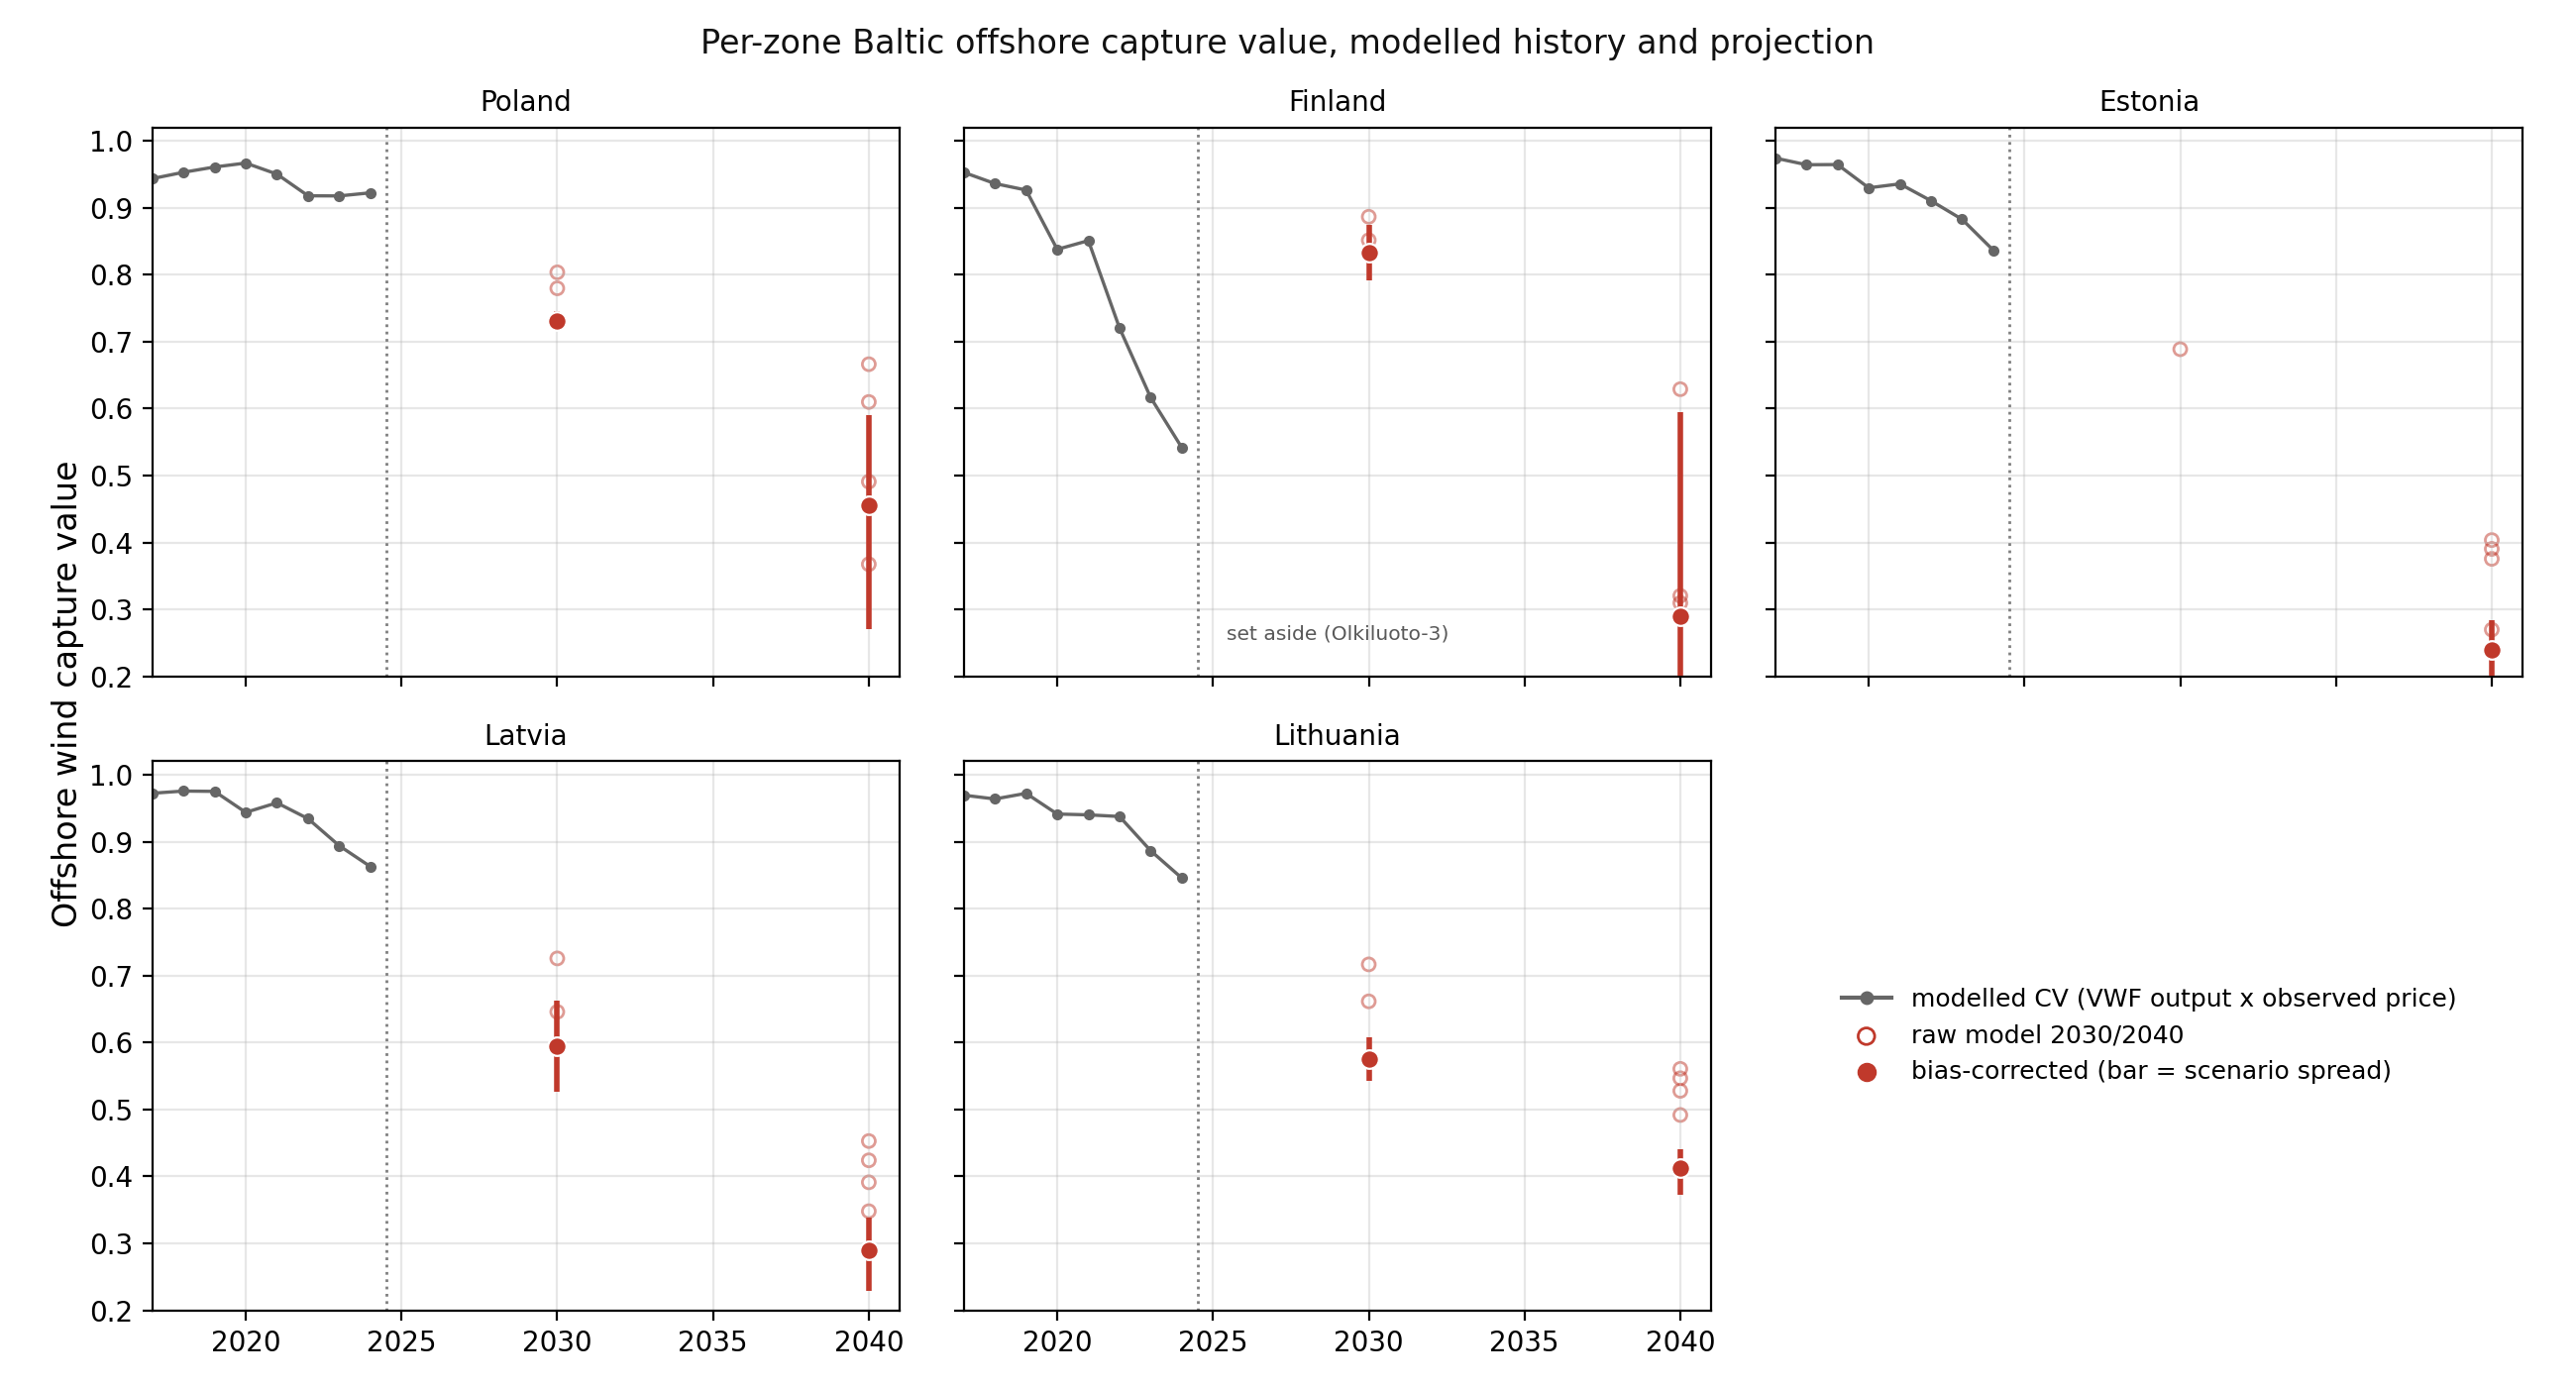
\includegraphics[width=0.98\textwidth]{fig_perzone_projection}
    \caption{Per-zone Baltic offshore capture value, modelled history (2017 to
    2024, grey; virtual-farm output weighted by observed zone prices, as no metered revenue
    exists) to bias-corrected projection (red), for the zones that build out
    (Finland shown but set aside, nuclear-driven). Open markers are the raw model;
    filled markers the bias-corrected central value; vertical bars the spread
    across scenarios at each horizon. The regression model stops responding at these horizons; these are
    system-model projections.}
    \label{fig:perzone}
\end{figure}

\subsection*{C.1 Full algorithm and validation-scheme comparison (regression model)}

Table~\ref{tab:regression_full} extends the headline metrics of
Table~\ref{tab:regression_metrics} to all five algorithm families under every
validation scheme. Gradient boosting leads on every genuine generalisation
test, and the polynomial's large negative out-of-fold scores show how violently a
closed form extrapolates, the instability that makes the tree the operational
model and the analytical equation only an interpretable backup.

\begin{table}[!htb]
\centering\small
\caption{Out-of-fold $R^2$ of all five algorithm families under every validation
scheme, at bidding-zone feature resolution. A dash marks schemes run only for
the headline model. These metrics are independent of the system-model re-solve.}
\label{tab:regression_full}
\begin{tabular}{l r r r r r}
\toprule
\textbf{Validation scheme} & \textbf{XGBoost} & \textbf{Random forest} & \textbf{SVR} &
\textbf{Poly(2)} & \textbf{Linear} \\
\midrule
Random K-fold (Jacquet scheme)    & 0.752 & 0.682 & 0.583 & 0.437 & 0.330 \\
Leave-farm-out (headline)           & \textbf{0.686} & 0.636 & 0.497 & $-19.9$ & 0.270 \\
Leave-farm-out, excluding 2022      & 0.692 & --- & --- & --- & --- \\
North Sea $\rightarrow$ Baltic      & 0.379 & 0.331 & 0.196 & $-12.2$ & 0.230 \\
Baltic $\rightarrow$ North Sea      & 0.139 & 0.204 & $-0.56$ & $-1.06$ & 0.020 \\
Time split (train $\le$2022, test 23--24) & $-0.03$ & --- & --- & --- & --- \\
\bottomrule
\end{tabular}
\end{table}

\subsection*{C.2 Baseline capture-value calibration, three years}

Table~\ref{tab:calibration_full} gives the per-zone calibration behind
Section~\ref{sec:trust_system} and the bias correction. The bias (PyPSA minus
observed) is near zero in the large North Sea zones and grows with congestion,
peaking in DK2 in both 2023 and 2024; these fifteen points are exactly what the
correction of Appendix~\ref{app:robustness} is fitted on. Because the baselines use
observed fleets, they are unaffected by the projection re-solve.

\begin{table}[!htb]
\centering\small
\caption{System-model capture value against observation, per zone and year, on
common hours. Observed pairs metered offshore generation with observed prices;
PyPSA is fully modelled; the hybrid prices modelled generation at observed prices,
localising any error to the wind or the price. Bias is PyPSA minus observed.}
\label{tab:calibration_full}
\begin{tabular}{l r r r r}
\toprule
\textbf{Zone} & \textbf{Observed} & \textbf{PyPSA} & \textbf{Hybrid} & \textbf{Bias} \\
\midrule
\multicolumn{5}{l}{\textit{2019 (pre-crisis)}} \\
DE  & 0.923 & 0.984 & 0.929 & $+0.061$ \\
NL  & 0.977 & 0.986 & 0.978 & $+0.010$ \\
BE  & 0.920 & 0.983 & 0.956 & $+0.064$ \\
DK1 & 0.924 & 0.986 & 0.944 & $+0.062$ \\
DK2 & 0.933 & 0.987 & 0.954 & $+0.054$ \\
\addlinespace
\multicolumn{5}{l}{\textit{2023 (headline validation)}} \\
DE  & 0.909 & 0.908 & 0.896 & $-0.001$ \\
NL  & 0.881 & 0.883 & 0.897 & $+0.002$ \\
BE  & 0.869 & 0.896 & 0.910 & $+0.027$ \\
DK1 & 0.854 & 0.917 & 0.869 & $+0.064$ \\
DK2 & 0.784 & 0.927 & 0.815 & $+0.143$ \\
\addlinespace
\multicolumn{5}{l}{\textit{2024 (most recent)}} \\
DE  & 0.910 & 0.941 & 0.875 & $+0.031$ \\
NL  & 0.900 & 0.919 & 0.884 & $+0.019$ \\
BE  & 0.893 & 0.928 & 0.913 & $+0.035$ \\
DK1 & 0.843 & 0.947 & 0.837 & $+0.104$ \\
DK2 & 0.808 & 0.949 & 0.821 & $+0.141$ \\
\bottomrule
\end{tabular}
\end{table}

% Pending the corrected-onshore re-solve: projected per-zone CV by scenario, the
% gas-shock grid, the scarcity decomposition, the surrogate per-zone metrics, and
% the full-versus-3-hourly resolution check. To be added once re-solved numbers land.


\subsection*{C.3 The sector-coupled arms, per zone}

Table~\ref{tab:sector_zones} details the matched twelve-hour pair behind
Table~\ref{tab:sector}: the electricity-only and sector-coupled solves of the
pinned 2040 TYNDP fleet, zone by zone. The cost-optimal arms behind them build
52 and 127~GW of offshore respectively and hold capture value near 0.8; the
pinned pair carries the comparison because its fleet matches the main
projection. At 2030 the sector-coupled solve gives a North Sea of 0.81 and a
Baltic of 0.86, within a few points of the electricity-only projection, so the
flexibility effect, like the grid's, appears only once the buildout binds. DK2
is excluded: the pinning fixes country totals, so its small allocated fleet is
not comparable across arms (Section~\ref{sec:sector_method}).

\begin{table}[!htb]
\centering\small
\caption{The matched 2040 twelve-hour solves, per zone: capture value and the
share of wind energy produced into zero-priced hours, electricity-only against
sector-coupled.}
\label{tab:sector_zones}
\begin{tabular}{l c c c c}
\toprule
& \multicolumn{2}{c}{\textbf{Capture value}} &
\multicolumn{2}{c}{\textbf{Zero-price share (\%)}} \\
\textbf{Zone} & \textbf{Electricity} & \textbf{Sector} & \textbf{Electricity} &
\textbf{Sector} \\
\midrule
DE  & 0.40 & 0.72 & 57 & 25 \\
NL  & 0.48 & 0.70 & 42 & 19 \\
BE  & 0.71 & 0.82 & 3  & 10 \\
DK1 & 0.38 & 0.74 & 77 & 20 \\
FR  & 0.80 & 0.84 & 6  & 1  \\
PL  & 0.65 & 0.85 & 18 & 28 \\
EE  & 0.39 & 0.77 & 45 & 20 \\
LV  & 0.41 & 0.82 & 41 & 20 \\
LT  & 0.37 & 0.81 & 43 & 21 \\
\bottomrule
\end{tabular}
\end{table}

\subsection*{C.4 Who bears the loss, by zone}

Table~\ref{tab:whopays_zones} resolves the three regimes of
Section~\ref{sec:whopays_results} zone by zone: scarcity-priced Poland, whose
low capture value coexists with a small unpaid share; the locally oversupplied
eastern Baltic, whose high unpaid shares the grid barely relieves; and the
open North Sea, whose shares the grid does relieve. Curtailment is the share
of available energy spilled, the volume channel that capture value cannot see
and Article~13 compensates.

\begin{table}[!htb]
\centering\small
\caption{The 2040 zero-price exposure by zone: capture value, the share of
wind energy in zero-priced hours, and the curtailed share of available energy,
on the frozen and the cost-optimal grid.}
\label{tab:whopays_zones}
\begin{tabular}{l c c c c c}
\toprule
& \multicolumn{3}{c}{\textbf{Frozen grid}} &
\multicolumn{2}{c}{\textbf{Optimal grid}} \\
\textbf{Zone} & \textbf{CV} & \textbf{Zero-price \%} & \textbf{Curtailed \%} &
\textbf{CV} & \textbf{Zero-price \%} \\
\midrule
DE  & 0.59 & 47 & 44 & 0.63 & 34 \\
NL  & 0.57 & 56 & 36 & 0.58 & 44 \\
BE  & 0.55 & 5  & 0  & 0.62 & 23 \\
DK1 & 0.55 & 69 & 18 & 0.84 & 36 \\
FR  & 0.56 & 32 & 20 & 0.68 & 28 \\
PL  & 0.49 & 6  & 1  & 0.74 & 32 \\
EE  & 0.39 & 42 & 2  & 0.53 & 39 \\
LV  & 0.42 & 37 & 5  & 0.59 & 33 \\
LT  & 0.49 & 30 & 12 & 0.59 & 31 \\
\bottomrule
\end{tabular}
\end{table}

\subsection*{C.5 The candidate areas, ranked}

Table~\ref{tab:site_table} lists the ten development areas behind
Figure~\ref{fig:site_ranking} at the 2040 horizon: levelised cost, capture
value, the resulting break-even price, and the two rankings whose divergence
the body reports (a rank correlation of 0.99 in 2025 falling to 0.90 by 2040).

\begin{table}[!htb]
\centering\small
\caption{The ten candidate development areas in 2040, ordered by
value-adjusted cost. The last column gives each area's value rank in 2025,
so a change between the two final columns is the reordering the horizon
produces.}
\label{tab:site_table}
\begin{tabular}{l c c c c c c}
\toprule
\textbf{Area} & \textbf{LCOE} & \textbf{CV} & \textbf{vLCOE} &
\textbf{Cost rank} & \textbf{Value rank} & \textbf{Value rank 2025} \\
& \euro/MWh & & \euro/MWh & & & \\
\midrule
German Bight        & 41 & 0.59 & 69  & 1  & 1  & 1 \\
Danish Baltic (DK2) & 46 & 0.57 & 80  & 3  & 2  & 4 \\
Polish Baltic       & 43 & 0.49 & 88  & 2  & 3  & 2 \\
Belgian             & 49 & 0.55 & 89  & 4  & 4  & 3 \\
Dutch North Sea     & 61 & 0.57 & 107 & 6  & 5  & 6 \\
French              & 68 & 0.56 & 120 & 7  & 6  & 7 \\
Estonian            & 51 & 0.39 & 130 & 5  & 7  & 5 \\
Danish North Sea    & 78 & 0.55 & 142 & 10 & 8  & 10 \\
Lithuanian          & 71 & 0.49 & 144 & 9  & 9  & 9 \\
Latvian             & 69 & 0.42 & 164 & 8  & 10 & 8 \\
\bottomrule
\end{tabular}
\end{table}

\section{Robustness of the Projection}\label{app:robustness}

The headline projection of Section~\ref{sec:projection_results} rests on the uncorrected
frozen-grid system model, with the penetration bias correction and the
parametric hydrogen-demand assumption reported as refinements. This appendix tests both, prices the
gas exposure, and sweeps the wider scenario space with the fast approximation of the system
model; none of
it moves the conclusion.

\subsection*{The bias correction is anchored on DK2}

\begin{figure}[!htb]
    \centering
    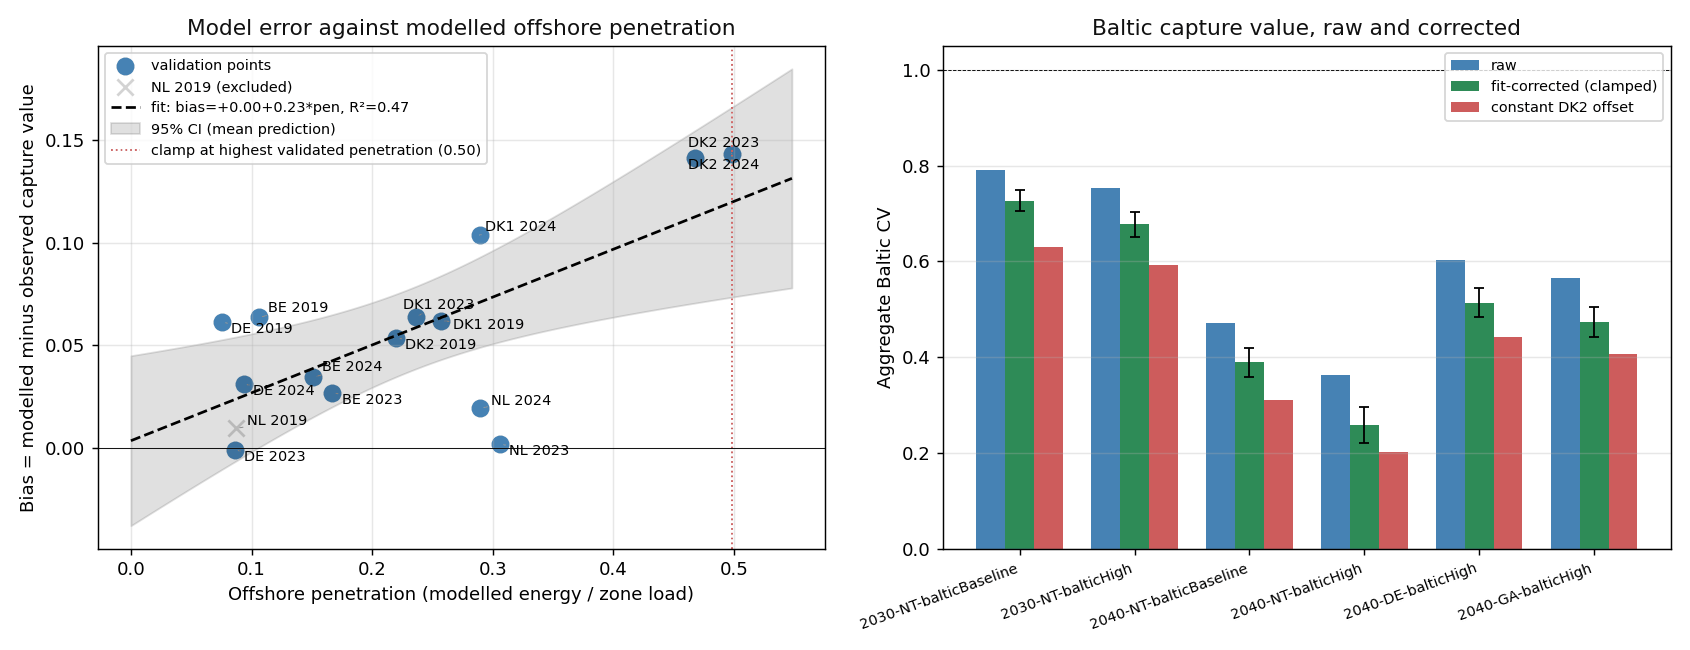
\includegraphics[width=0.95\textwidth]{fig_bias_fit_and_corrected}
    \caption{The bias correction and its effect: the validation bias against
    modelled penetration, anchored by DK2 (left), and raw against corrected
    Baltic capture value per scenario (right).}
    \label{fig:bias_corrected}
\end{figure}

The correction of Section~\ref{sec:bias_method} fits the model's capture-value
overstatement against its own offshore penetration on fourteen validation points
(five zones in 2019, 2023 and 2024, the Netherlands 2019 excluded). Only the two
DK2 entries lie above 31\,\% penetration, so the slope is a line between a
structureless low-penetration cloud and a single high-penetration zone
(Figure~\ref{fig:lozo}). Leave-one-zone-out makes this explicit
(Table~\ref{tab:lozo}): dropping any zone except DK2 leaves the slope between
0.22 and 0.28 with its 95\,\% interval clear of zero, while dropping DK2
collapses it from 0.233 to 0.045, sends the interval across zero, and drops the
penetration term's $R^2$ from 0.47 to 0.02. The penetration dependence is,
statistically, the statement that DK2 has a large bias at a high penetration.

The conclusion nonetheless survives, because the correction is not what produces
it. The uncorrected model already lands at 0.36--0.60 in 2040; the DK2-removed
correction is a near-constant offset of about 0.05 that takes it to 0.31--0.56;
the full correction reaches 0.26--0.51. All three agree on a loss of at least a
third of present capture value, and near half in the central scenario. DK2 is
kept as the anchor precisely because it
is the only existing high-penetration, Baltic-facing zone, which is what makes it
the right analogue and, at the same time, why the correction cannot be claimed as
a calibrated law. Reproduced by \texttt{1.19\_bias\_correction\_robustness.py}.

\begin{figure}[!htb]
    \centering
    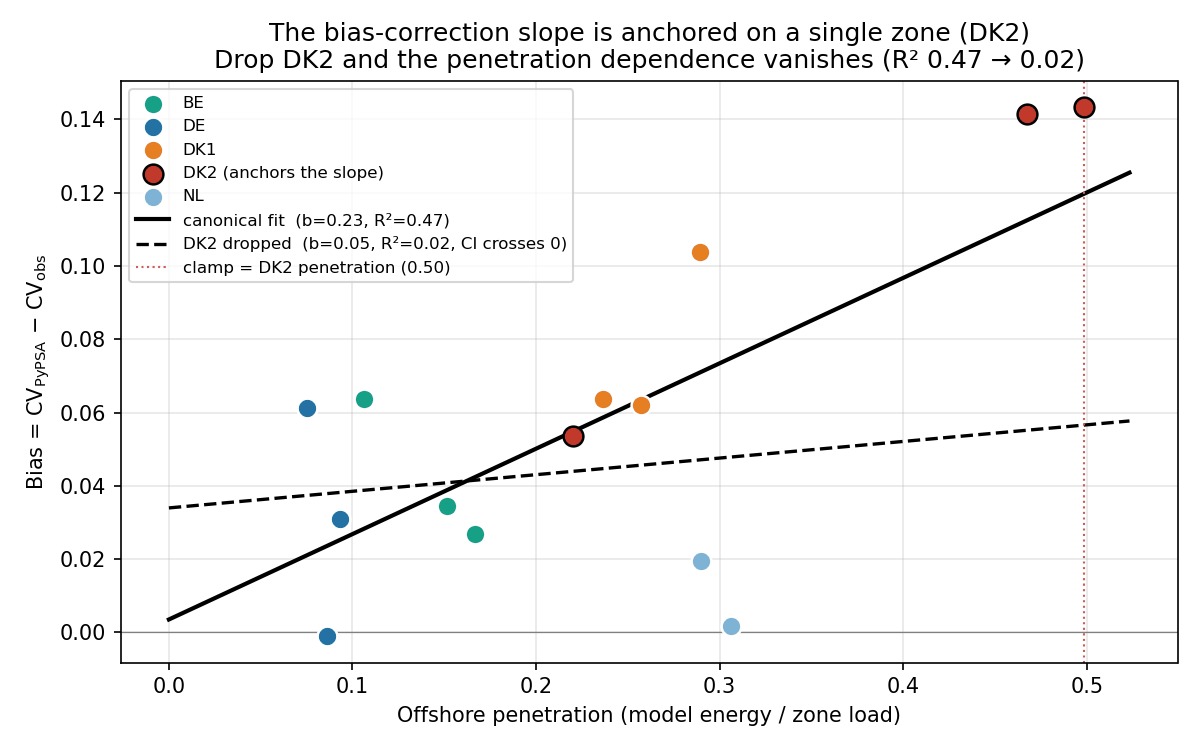
\includegraphics[width=0.8\textwidth]{fig_bias_lozo}
    \caption{The bias-correction slope is anchored on a single zone. The fourteen
    validation points (coloured by zone), the canonical fit, and the fit with DK2
    removed; without DK2 the penetration dependence vanishes ($R^2$ 0.47 to 0.02)
    and the slope's interval crosses zero.}
    \label{fig:lozo}
\end{figure}

\begin{table}[!htb]
\centering\small
\caption{Leave-one-zone-out and (last three rows) leave-one-year-out refits of
the bias slope. The slope and its 95\,\% interval are stable to dropping any zone
except DK2, whose removal collapses both.}
\label{tab:lozo}
\begin{tabular}{l c c c c}
\toprule
\textbf{Refit} & \textbf{$n$} & \textbf{Slope} & \textbf{95\,\% CI} &
\textbf{$R^2$} \\
\midrule
Canonical (all 14) & 14 & 0.233 & [0.08, 0.39] & 0.47 \\
Drop DE  & 11 & 0.262 & [0.05, 0.48] & 0.46 \\
Drop NL  & 12 & 0.278 & [0.18, 0.38] & 0.79 \\
Drop BE  & 11 & 0.251 & [0.06, 0.44] & 0.50 \\
Drop DK1 & 11 & 0.224 & [0.04, 0.40] & 0.46 \\
\textbf{Drop DK2} & 11 & \textbf{0.045} & \textbf{[$-$0.21, 0.30]} & \textbf{0.02} \\
\midrule
Drop 2019 & 10 & 0.303 & [0.11, 0.49] & 0.63 \\
Drop 2023 & 9 & 0.200 & [$-$0.00, 0.40] & 0.43 \\
Drop 2024 & 9 & 0.195 & [$-$0.04, 0.43] & 0.36 \\
\bottomrule
\end{tabular}
\end{table}


\subsection*{The DK2 price shape is outside the model class}

The bias correction treats the DK2 overstatement as a measured error. The
alternative, repairing the dispatch until DK2 comes out right, was tried
exhaustively and failed, which is what justifies the treatment
(Table~\ref{tab:dk2_experiments}). The blocking mechanism is structural: DK2
retains about 2,900~MW of export capacity into a Nordic system holding 62~TWh
of reservoir hydro, so a local surplus always finds a positive-priced sink and
the zonal price never collapses. The observed shape, 264 negative-price hours
in 2023, is produced by unit commitment, must-run combined heat and power, and
subsidised bidding, none of which a linear program contains.
Figure~\ref{fig:dk2_mechanism} shows the diagnosis: the model's generation is
right and its prices are too flat in exactly the windy hours. The model
that does land DK2 is the regression, out of fold at 0.798 against the
observed 0.784.

\begin{table}[!htb]
\centering\small
\caption{The DK2 re-dispatch experiments. No dispatch-side change
reproduces the observed 0.784; the shape needs mechanisms a linear program
does not contain. Values are DK2 capture value unless stated.}
\label{tab:dk2_experiments}
\begin{tabular}{p{3.6cm} p{4.4cm} p{5.6cm}}
\toprule
\textbf{Experiment} & \textbf{Change} & \textbf{Outcome} \\
\midrule
Faithful re-solve & none & 0.927 to 0.968: the price is not even unique \\
Negative wind bids & $-60$~\euro/MWh region-wide & no change: hydro absorbs the surplus \\
Derate the {\"O}resund alone & 3,396 to 1,700~MW & backfires: mean price 38 to 98~\euro/MWh, re-pinned to German gas \\
Myopic hydro & reservoirs capped at 24~h & explodes: 0.58 at a 1,207~\euro/MWh mean price \\
Market NTCs, both corridors & DK2--SE 1,700, DE--DK1 2,500~MW & DK1 error $+0.06$ to $+0.01$; DK2 unmoved at $+0.15$ \\
Rolling-horizon hydro & twelve monthly solves, 14-day lookahead & backwards: 0.932 to 0.957 \\
Must-run heat $\times$ negative bids (nine-point grid) & minimum load 0.20 to 0.50, bids 0 to $-10$~\euro/MWh & 0.947 to 0.958 across all nine; zero negative-price hours \\
\bottomrule
\end{tabular}
\end{table}

\begin{figure}[!htb]
    \centering
    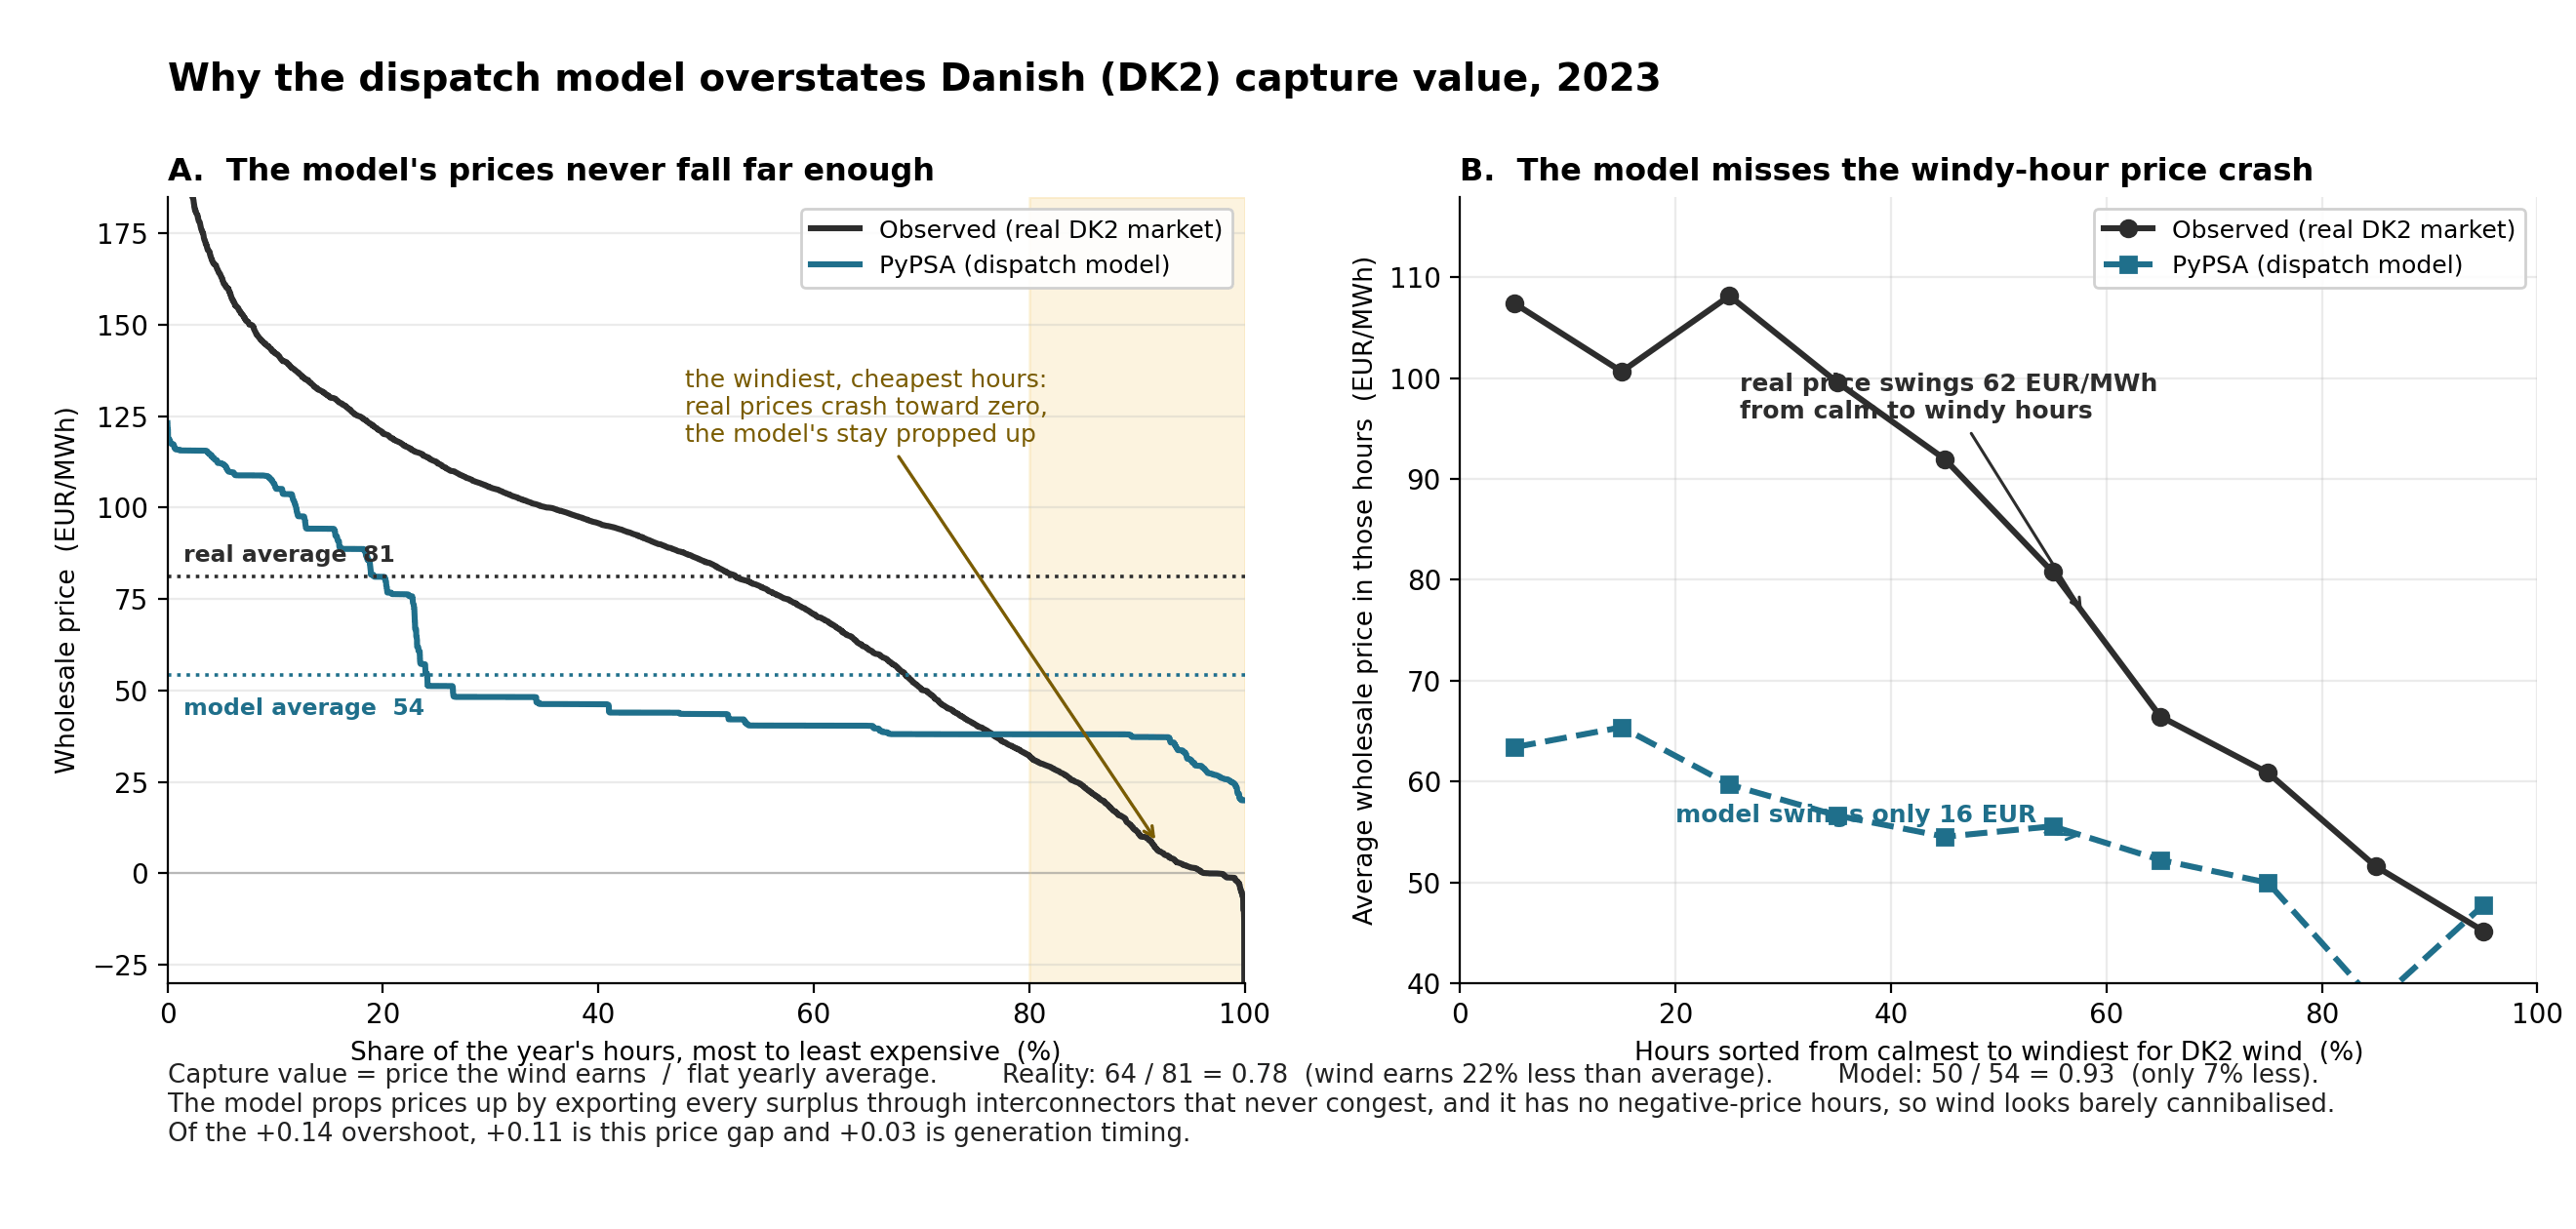
\includegraphics[width=0.9\textwidth]{fig_dk2_capturevalue_mechanism}
    \caption{The DK2 diagnosis. Pricing the model's own generation at observed
    prices recovers the observed capture value, so the wind is right and the
    error lives entirely in the price shape, which stays flat in the windy
    hours where real DK2 prices collapse.}
    \label{fig:dk2_mechanism}
\end{figure}

\subsection*{The hydrogen-demand assumption does not drive the result}

Correction D adds a parametric hydrogen layer that holds prices off zero at high
renewable shares; its demand is assumed, so the 2040 result is tested against it
by re-solving every 2040 scenario with the electrolyser demand and capacity
scaled to half and one-and-a-half times the canonical level
(Figure~\ref{fig:h2sens}). Across that $\pm 50\,\%$ range the energy-weighted
Baltic capture value moves by at most 0.013 in any scenario and by under 0.01 in
the two cannibalisation-dominated DE and GA scenarios; the 2040 band shifts only
from 0.36--0.60 at the central floor to 0.37--0.60 at either
extreme. Load-shed volumes are unchanged across the variants, so the small
sensitivity that does exist runs through the price floor and not through
adequacy: more hydrogen demand lifts the windy-hour prices where wind earns, so
capture value rises slightly. The floor sets the depth of the erosion at the
margin; it does not create it. Reproduced by
\texttt{1.20\_h2\_floor\_sensitivity.py}.

\begin{figure}[!htb]
    \centering
    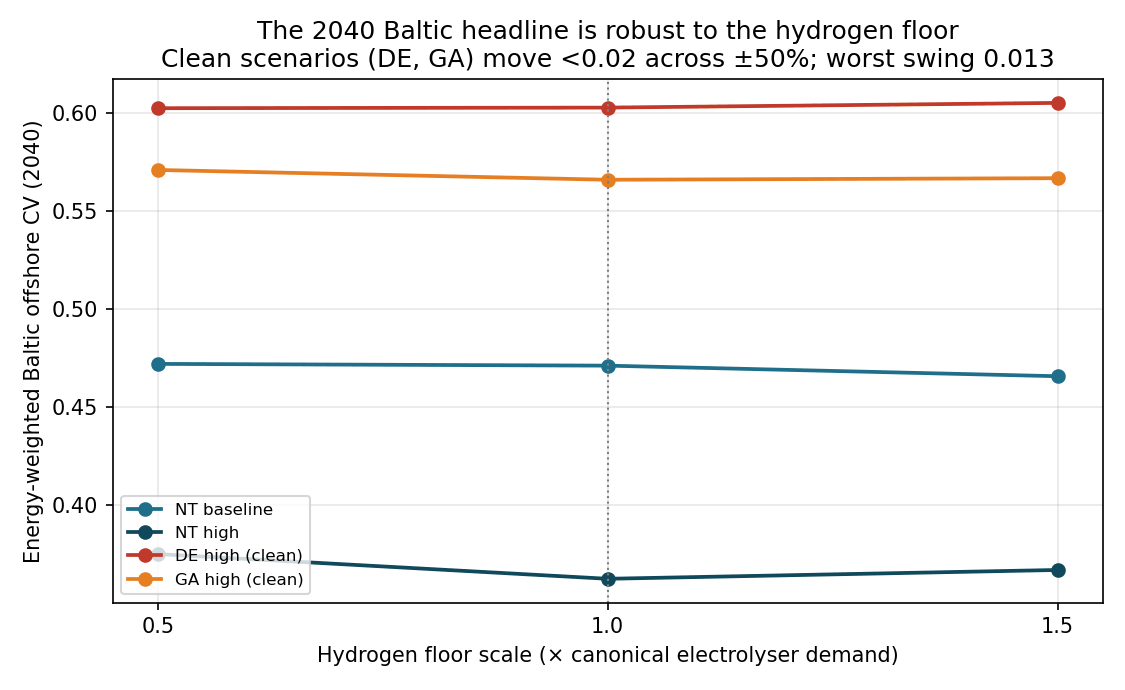
\includegraphics[width=0.8\textwidth]{fig_h2_sensitivity}
    \caption{The 2040 Baltic capture value against the scale of the assumed hydrogen demand (half to one-and-a-half times the
    central electrolyser demand). The clean
    DE and GA scenarios are nearly flat; the NT scenarios carry a small,
    floor-mediated dependence; the headline survives across the range.}
    \label{fig:h2sens}
\end{figure}

\subsection*{The gas-price grid}\label{sec:gas_results}

One input remains untested: the gas price that set every European record in 2022.
Re-solving three buildout scenarios across five gas prices, 15 to 120~\euro/MWh,
prices the exposure directly (Figure~\ref{fig:gas_cv}). The grid is coarse, fifteen networks, so the slopes indicate direction only. In 2030 the North Sea is the more exposed basin and the
Baltic is already near-decoupled: gas still sets the price often in the thermal
North Sea, rarely in the windy Baltic hours. Even end to end, the full crisis
sweep moves the 2030 North Sea capture value by only 0.07, less than one step of
the buildout. By 2040 both basins decouple almost entirely, their prices set by renewables, the demand-response tier, and hydrogen
production. Gas risk is real, asymmetric, and second-order. The buildout drives Baltic
value, and the fuel price only modulates it.

\begin{figure}[!htb]
    \centering
    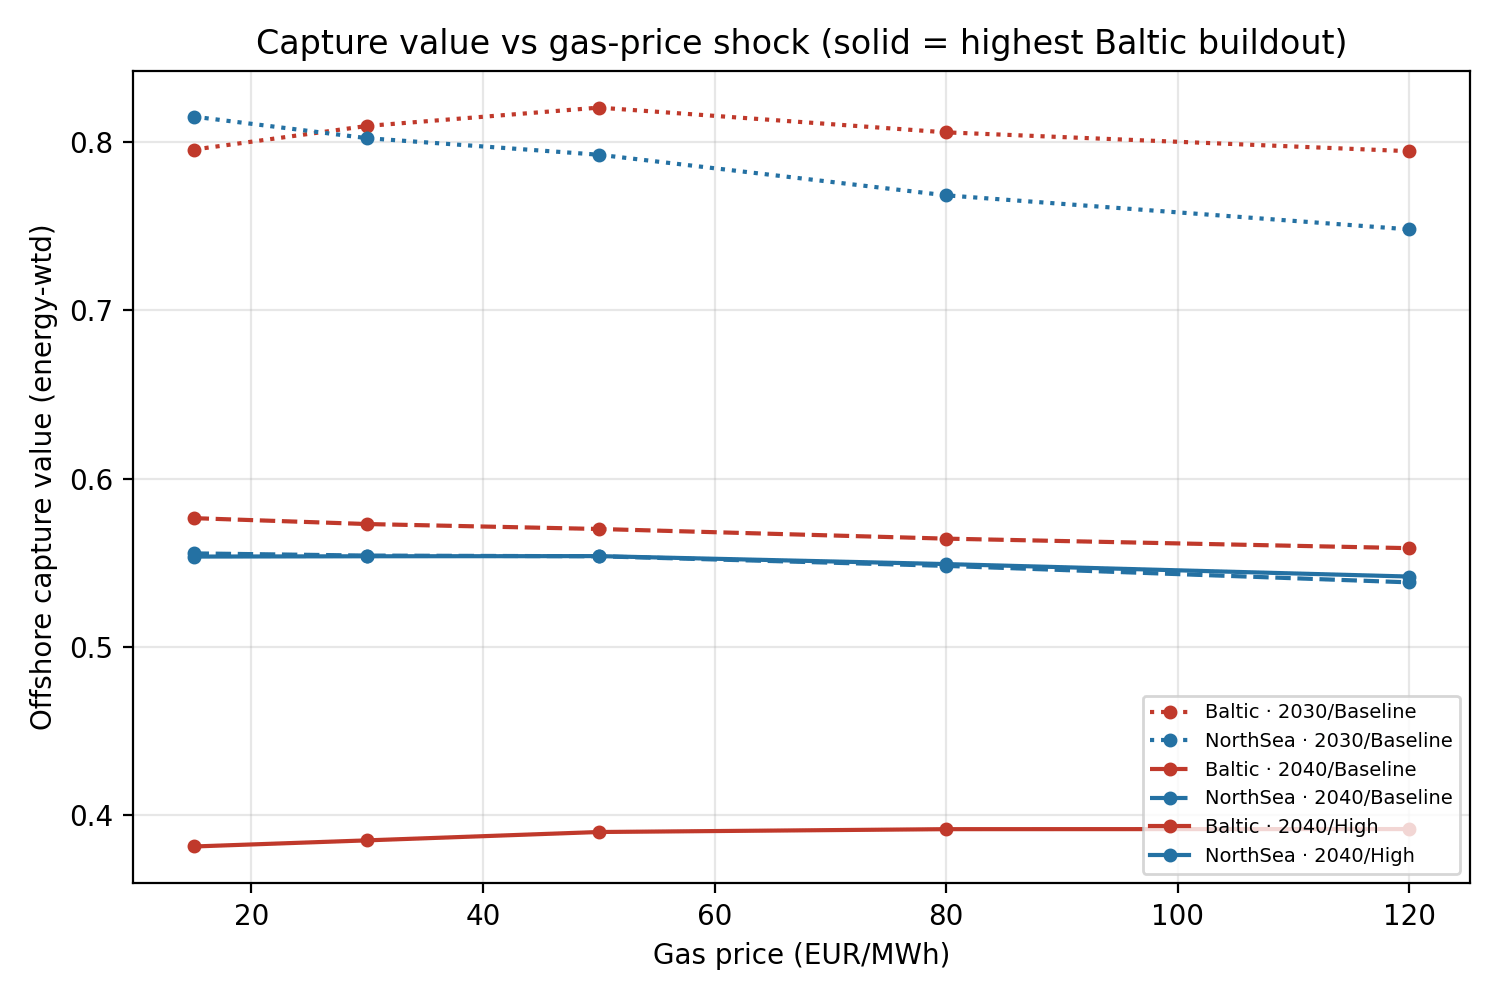
\includegraphics[width=0.92\textwidth]{fig_gas_shock_cv}
    \caption{Capture value across the gas-price grid, by basin and scenario. The
    North Sea's exposure is visible in 2030; the Baltic's curves are nearly flat,
    and by 2040 both basins decouple from gas.}
    \label{fig:gas_cv}
\end{figure}


\subsection*{The wider scenario sweep}

The fast approximation of the system model is a gradient-boosted model
trained on 76 solved networks
(the 55 dedicated training solves plus the 21 reused full-resolution baseline
and scenario solves of Table~\ref{tab:runs}), its inputs spread across the
scenario space by Latin hypercube sampling. Its training solves run
three-hourly; re-solving design points at full resolution confirms the
approximation is benign in the policy-relevant range and only optimistic at
the highest levels of buildout.

Its held-out skill is adequate for
exploration ($R^2$ 0.86 for capture value), it reproduces the 2040 scenarios to
within 0.05, and it leans optimistic beyond about 100~GW of Baltic offshore,
with the headline left to the direct solves throughout.

Across that space, buildout drives the erosion and gas barely moves it. The
Monte-Carlo draw (Figure~\ref{fig:montecarlo}), reaching beyond the plan to
150~GW, puts the median Baltic capture value at 0.28 and the
North-Sea-to-Baltic asymmetry near 2.3 times. The envelope samples
buildouts well beyond the official plans, to 150~GW, so its centre of mass is more
aggressive than any TYNDP scenario; that the direct solves sit in the upper half
of the distribution means the headline range is, if anything, conservative.
Nowhere in the explored space does heavy Baltic buildout coexist with a healthy
Baltic capture value.




\subsection{Weather-only corroboration}\label{sec:weather_agrees}

Features and capture values share market data, so the mechanism could be
circular. The weather is not. Clustering the farms by hourly output alone, no
prices and no market labels, the geography sorts them on its own
(Figure~\ref{fig:clusters}): North Sea zones correlate at 0.44, the
under-built Baltic states at 0.61, the built-out DK2 and SE4 at 0.87, and the
two basins are largely independent at 0.28. The grouping reflects meteorology,
and it points forward: the under-built zones, the ones the buildout will fill,
are a tightly-correlated bloc. The same signal
repeats inside countries: a compact fleet blows nearly as one (Belgium 0.96,
Poland 0.94) while a spread one does not (Germany 0.64, Denmark 0.67).
Germany's farms even split into a North Sea and a Baltic block, so the basin is the right boundary for the analysis (Appendix~\ref{app:supplementary}). The physical picture behind the
enclosure penalty is now complete: Baltic wind arrives together, into a smaller market with weaker export capacity.

\begin{figure}[!htb]
    \centering
    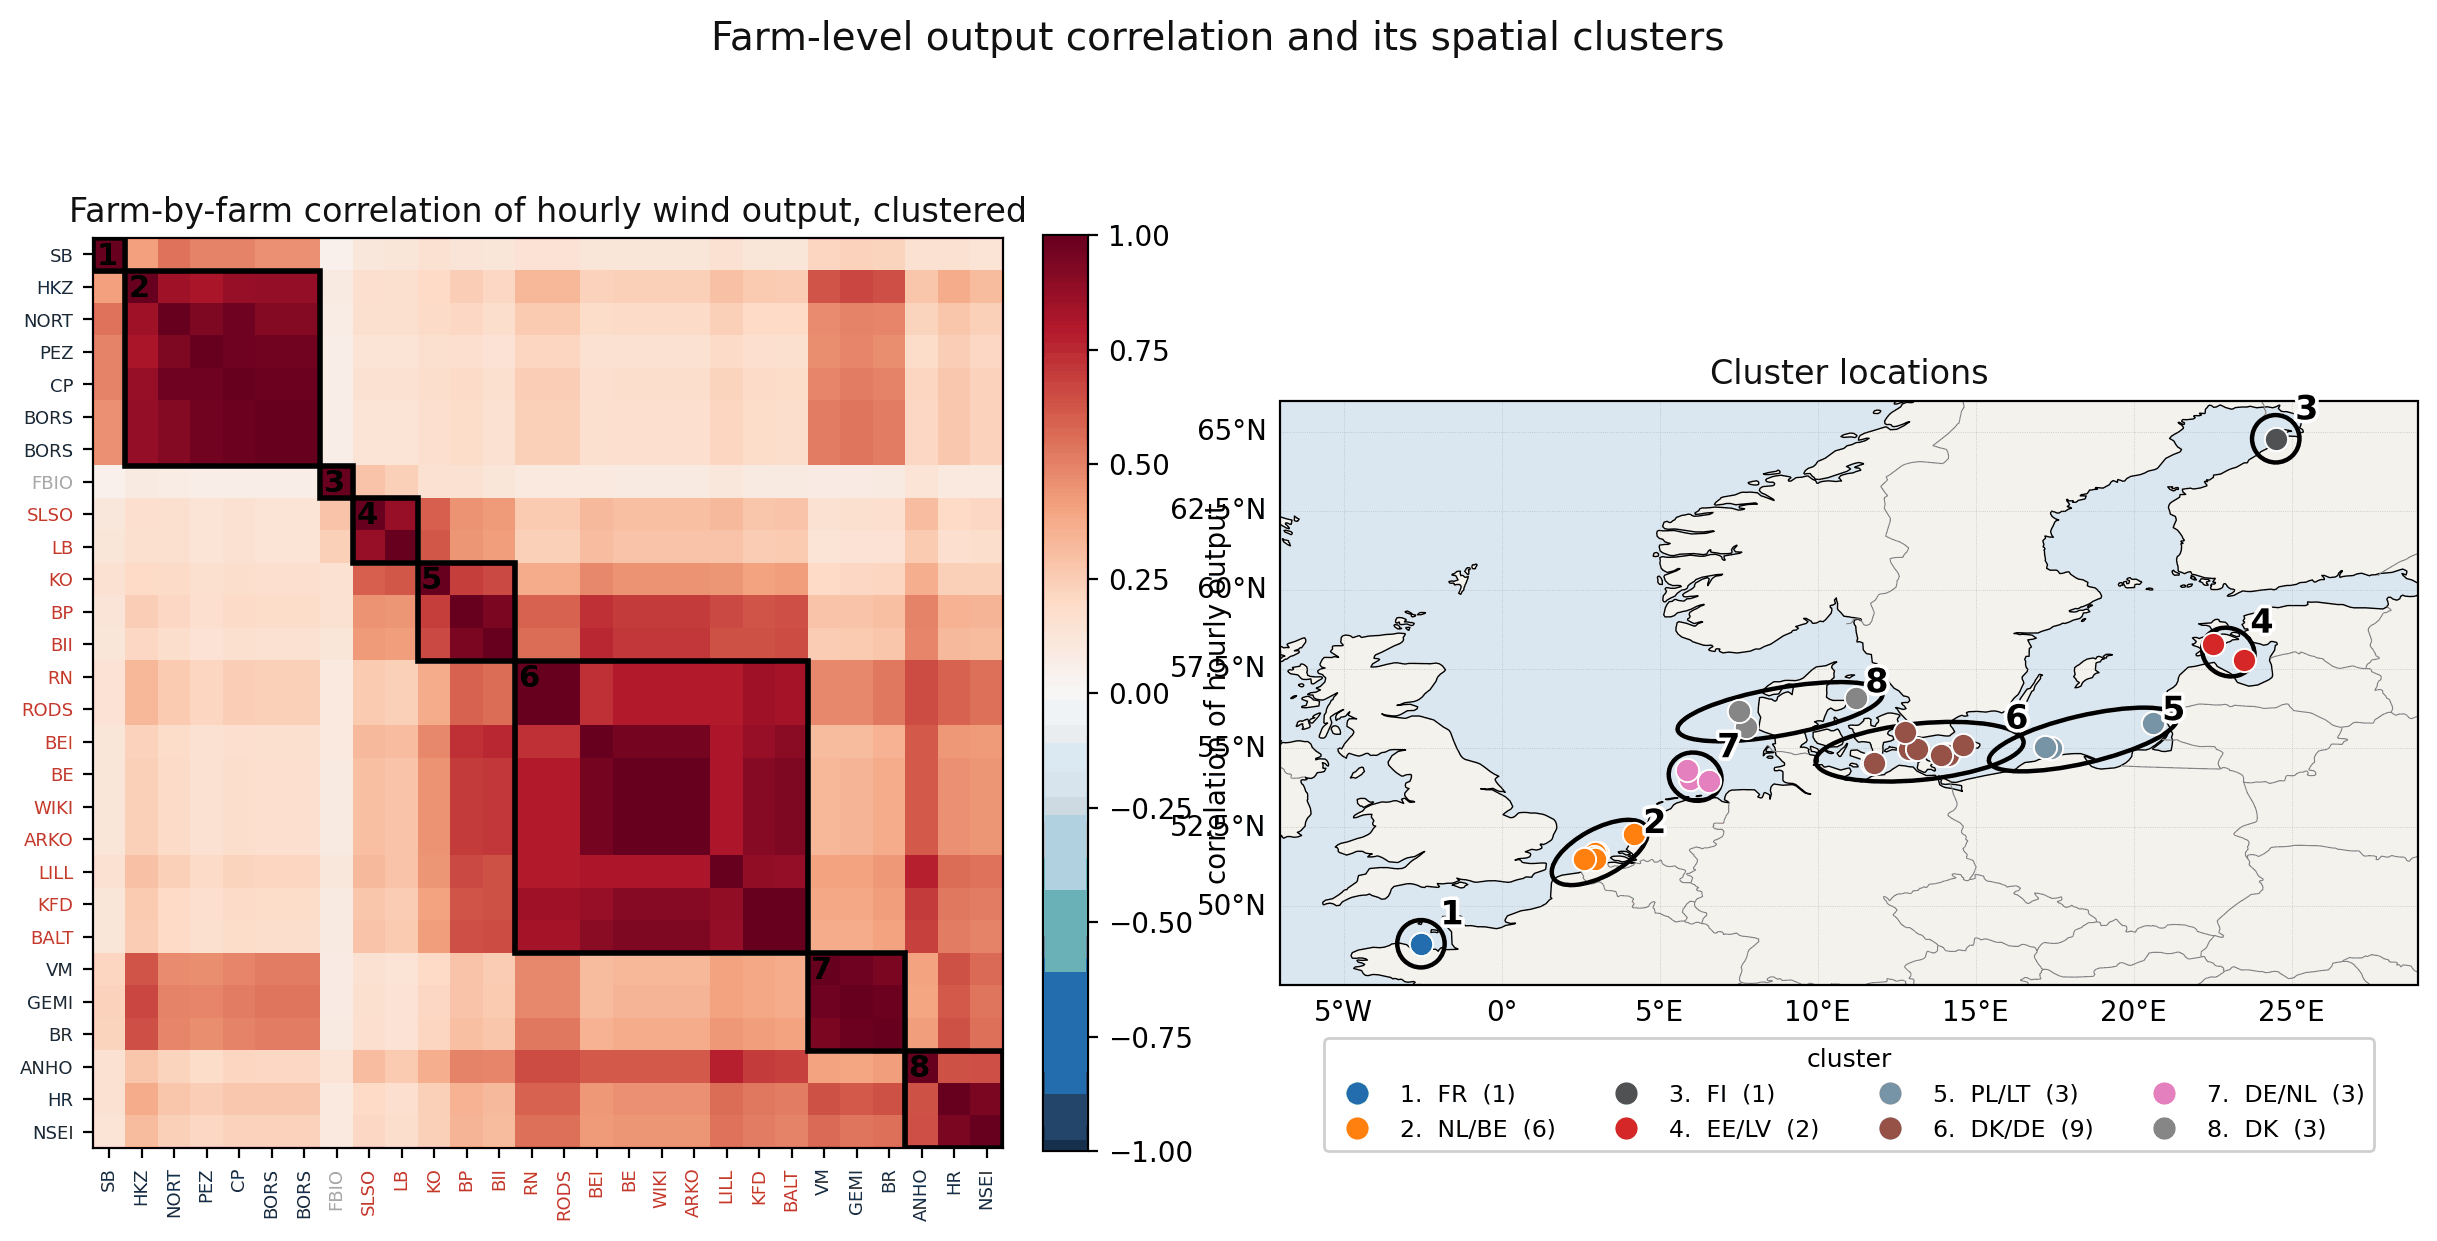
\includegraphics[width=0.98\textwidth]{fig_basin_correlation}
    \caption{Weather-only corroboration: hourly-output correlation clustered
    (left) and the clusters mapped (right). Within-basin correlation is high
    and cross-basin low: North Sea 0.44, under-built Baltic 0.61, built-out
    0.87, cross-basin 0.28.}
    \label{fig:clusters}
\end{figure}

That proximity reflects the mechanism itself. Plotting every farm pair's
output correlation against its separation collapses both basins onto a single
decay curve, correlation falling away with a fitted length of 422~km
(Figure~\ref{fig:corr_distance}). The Baltic pairs obey no different physics;
they sit on the near, steep end of the same curve because the basin's farms
are closer together (median 285~km against 347, a few long pairs
notwithstanding).
Distance sets synchronicity, and the Baltic's geography fixes the distance.

\subsection{Scarcity and gas sensitivities}\label{sec:scarcity_results}

The second movement begins by ruling out the rival explanations. Could the
2040 erosion be adequacy stress rather than cannibalisation?
Recomputing every capture value with scarcity-priced hours removed answers it
(Figure~\ref{fig:scarcity_bars}): the 2030 and clean 2040 scenarios barely
move, and the two NT scenarios, whose $+0.15$ adequacy component sits almost
entirely in Poland, still reach only 0.51 to 0.62,
far below today's 0.88. The floor of the range comes from cannibalisation alone.

Gas is the other suspect input, and it is second-order too. Re-solving three
buildouts across five gas prices, 15 to 120~\euro/MWh, moves the 2030 North
Sea capture value by only 0.07 end to end, less than one step of the buildout.
By 2040 both basins have decoupled from gas almost entirely, their prices set by renewables, demand response and hydrogen production
(Appendix~\ref{app:robustness}). Baltic value is set by the buildout, with fuel prices a second-order
influence.

\subsection{Sector coupling and flexible demand}\label{sec:sector_results}

The grid is the spatial escape for surplus wind; the temporal escape, heat,
hydrogen and storage absorbing windy hours locally, is excluded from the
electricity-only model by construction. A sector-coupled variant therefore
tests it against an electricity-only twin identical in every setting
(Section~\ref{sec:sector_method}), so the difference between the two solves
is the value of flexibility alone.

\begin{table}[!htb]
\centering
\caption{The value of flexible demand: the matched twelve-hour 2040 solves,
    TYNDP fleet pinned, frozen grid. Zero-price columns give the share of wind
    energy produced into zero-priced hours.}
\label{tab:sector}
\begin{tabular}{l c c c c}
\toprule
& \multicolumn{2}{c}{\textbf{Capture value}} &
\multicolumn{2}{c}{\textbf{Zero-price share}} \\
\textbf{2040 solve (12\,h)} & \textbf{North Sea} & \textbf{Baltic} &
\textbf{NS} & \textbf{Baltic} \\
\midrule
Electricity only & 0.51 & 0.54 & 45\,\% & 29\,\% \\
Sector-coupled   & 0.74 & 0.82 & 19\,\% & 25\,\% \\
Flexibility effect & $+0.23$ & $+0.28$ & & \\
\bottomrule
\end{tabular}
\end{table}

Flexibility recovers most of what the frozen grid destroys
(Table~\ref{tab:sector}): the isolated effect, $+0.23$ and $+0.28$, is the
same order as the grid lever, and it is again the Baltic that gains most,
ending above the open basin as local electrolysis absorbs its surplus. In 2030
the sector world sits within a few points of the electricity-only one, so
flexibility, like transmission, pays only once the erosion binds. Per-zone
values are in Appendix~\ref{app:tables}.

Two facts keep the headline in place: the zero-price problem shrinks but does
not vanish, 19 to 25\,\% of wind energy still unpaid in the sector-coupled
solves, so the contract question survives full flexibility; and the
twelve-hour resolution smooths the price shape both arms see, so these
numbers bracket the hourly headline rather than replace it. Read beside the two grid solves, the levers agree: the frozen electricity-only world is the
floor, and either escape lifts the Baltic off it further than the North
Sea.

\FloatBarrier
% ----------------------------------------------------------------------------


\subsection{Pricing scarcity}\label{sec:scarcity_method}

A stressed scenario must be able to not serve demand, and the price of that
choice shapes every average. Correction F sets the ladder, demand response at
five percent of peak load offered at 400~\euro/MWh and unserved energy at the
4,000~\euro/MWh cap, so scarcity hours price as the real market would, and
Section~\ref{sec:robustness} measures how much of each scenario's erosion is
scarcity rather than cannibalisation.

\subsection{The sector-coupled variant}\label{sec:sector_method}

The electricity-only model can move surplus wind only through space, over the
grid; real systems also move it through time and into other demands. To measure how much of the projected erosion flexible demand removes, the
system model is rebuilt in PyPSA-Eur's sector-coupled configuration,
heating, hydrogen, storage and electric transport co-optimised alongside
electricity for an overnight 2040 system. The full-sector problem is tractable
only at twelve-hour resolution, so its control is an electricity-only twin
solved at the same twelve hours with every other setting identical, both arms
pinned to the same TYNDP fleet, so the difference between the two solves is
the value of flexibility itself. Two limits qualify the reading: twelve-hour
steps smooth the price shape both arms see, and country-level pinning makes
small zones such as DK2 incomparable across arms
(Section~\ref{sec:sector_results}).

\section{The Two-Estimator Test}\label{app:two_estimators}

Section~\ref{sec:gap_decomposition} states why the two models diverge beyond
the observed record. This appendix carries the underlying test, which asks
whether the divergence follows from how each model is built rather than from
any disagreement about how prices form. The error types named here are
structural descriptions of each model's construction; the measured composition
of each model's error, on held-out targets, is the Theil partition reported in
Section~\ref{sec:skill}.


The division of labour has a mathematical basis, and it was tested
(Figure~\ref{fig:theory}). The regression is a bounded interpolator: four
hundred trees give a piecewise-constant surface whose output cannot leave the
training range and whose gradient is exactly zero outside it. The system
model is a linear program whose price is the shadow price of the nodal energy
balance, re-derived from the merit order every hour with no training range at
all, but floored at zero. Table~\ref{tab:error_anatomy} sets the two error
structures side by side.

\begin{table}[!htb]
\centering\small
\caption{The two error structures compared. Each row is measured in this
chapter or Appendix~\ref{app:robustness}; the mean signed errors are against
observed 2023--24 capture values.}
\label{tab:error_anatomy}
\begin{tabular}{p{3.2cm} p{5.3cm} p{5.3cm}}
\toprule
 & \textbf{Regression model} & \textbf{System model} \\
\midrule
Error type & Bounded interpolation & Simplified market \\
Mean signed error & $-0.005$ & $+0.057$ \\
Sign and shape & No systematic sign & Always overstates; grows with
congestion \\
Largest where & Outside the training support (all 36 projection rows) & Small,
hydro-coupled zones (DK2 $+0.14$) \\
Detected by & Range and convex-hull checks & Three-way comparison \\
Consequence & Returns a constant from 2040 & Corrected by the measured fit \\
\bottomrule
\end{tabular}
\end{table}

Three consequences follow, and the runs confirm each
(Table~\ref{tab:theory_numbers}). Outside the range of its training data the regression model returns a
constant: across the four Baltic 2040 scenarios its answers span 0.008 of
capture value where
the system model spans 0.43, a fifty-four-fold difference. The two agree
where both can be checked, to 0.06 in sample and 0.04 at 2030, and diverge to
0.35 at 2040, where the projection leaves the training support. And the
system model's error has a predictable sign and order: it overstates every
validated zone, most where zones are small and hydro-coupled, DK2 above DK1
above Belgium above Germany and the Netherlands, which is exactly the shape
the bias correction of Section~\ref{sec:bias_method} subtracts.

One expectation fails, and the failure is informative. The erosion was
expected to accelerate with penetration; the fitted response is the opposite,
a saturating curve, because the zero price floor caps how much a marginal
windy hour can still lose once the price already sits at zero. The saturation
means the system model, if anything, understates cannibalisation at extreme
penetration, so the 2040 numbers are upper bounds on capture value,
conservative in the same direction as the measured bias. The two models' errors are of different kinds, and the division of roles
places each model where its error is smallest. Section~\ref{sec:skill} measures
those kinds directly on held-out targets.

\begin{figure}[!htb]
    \centering
    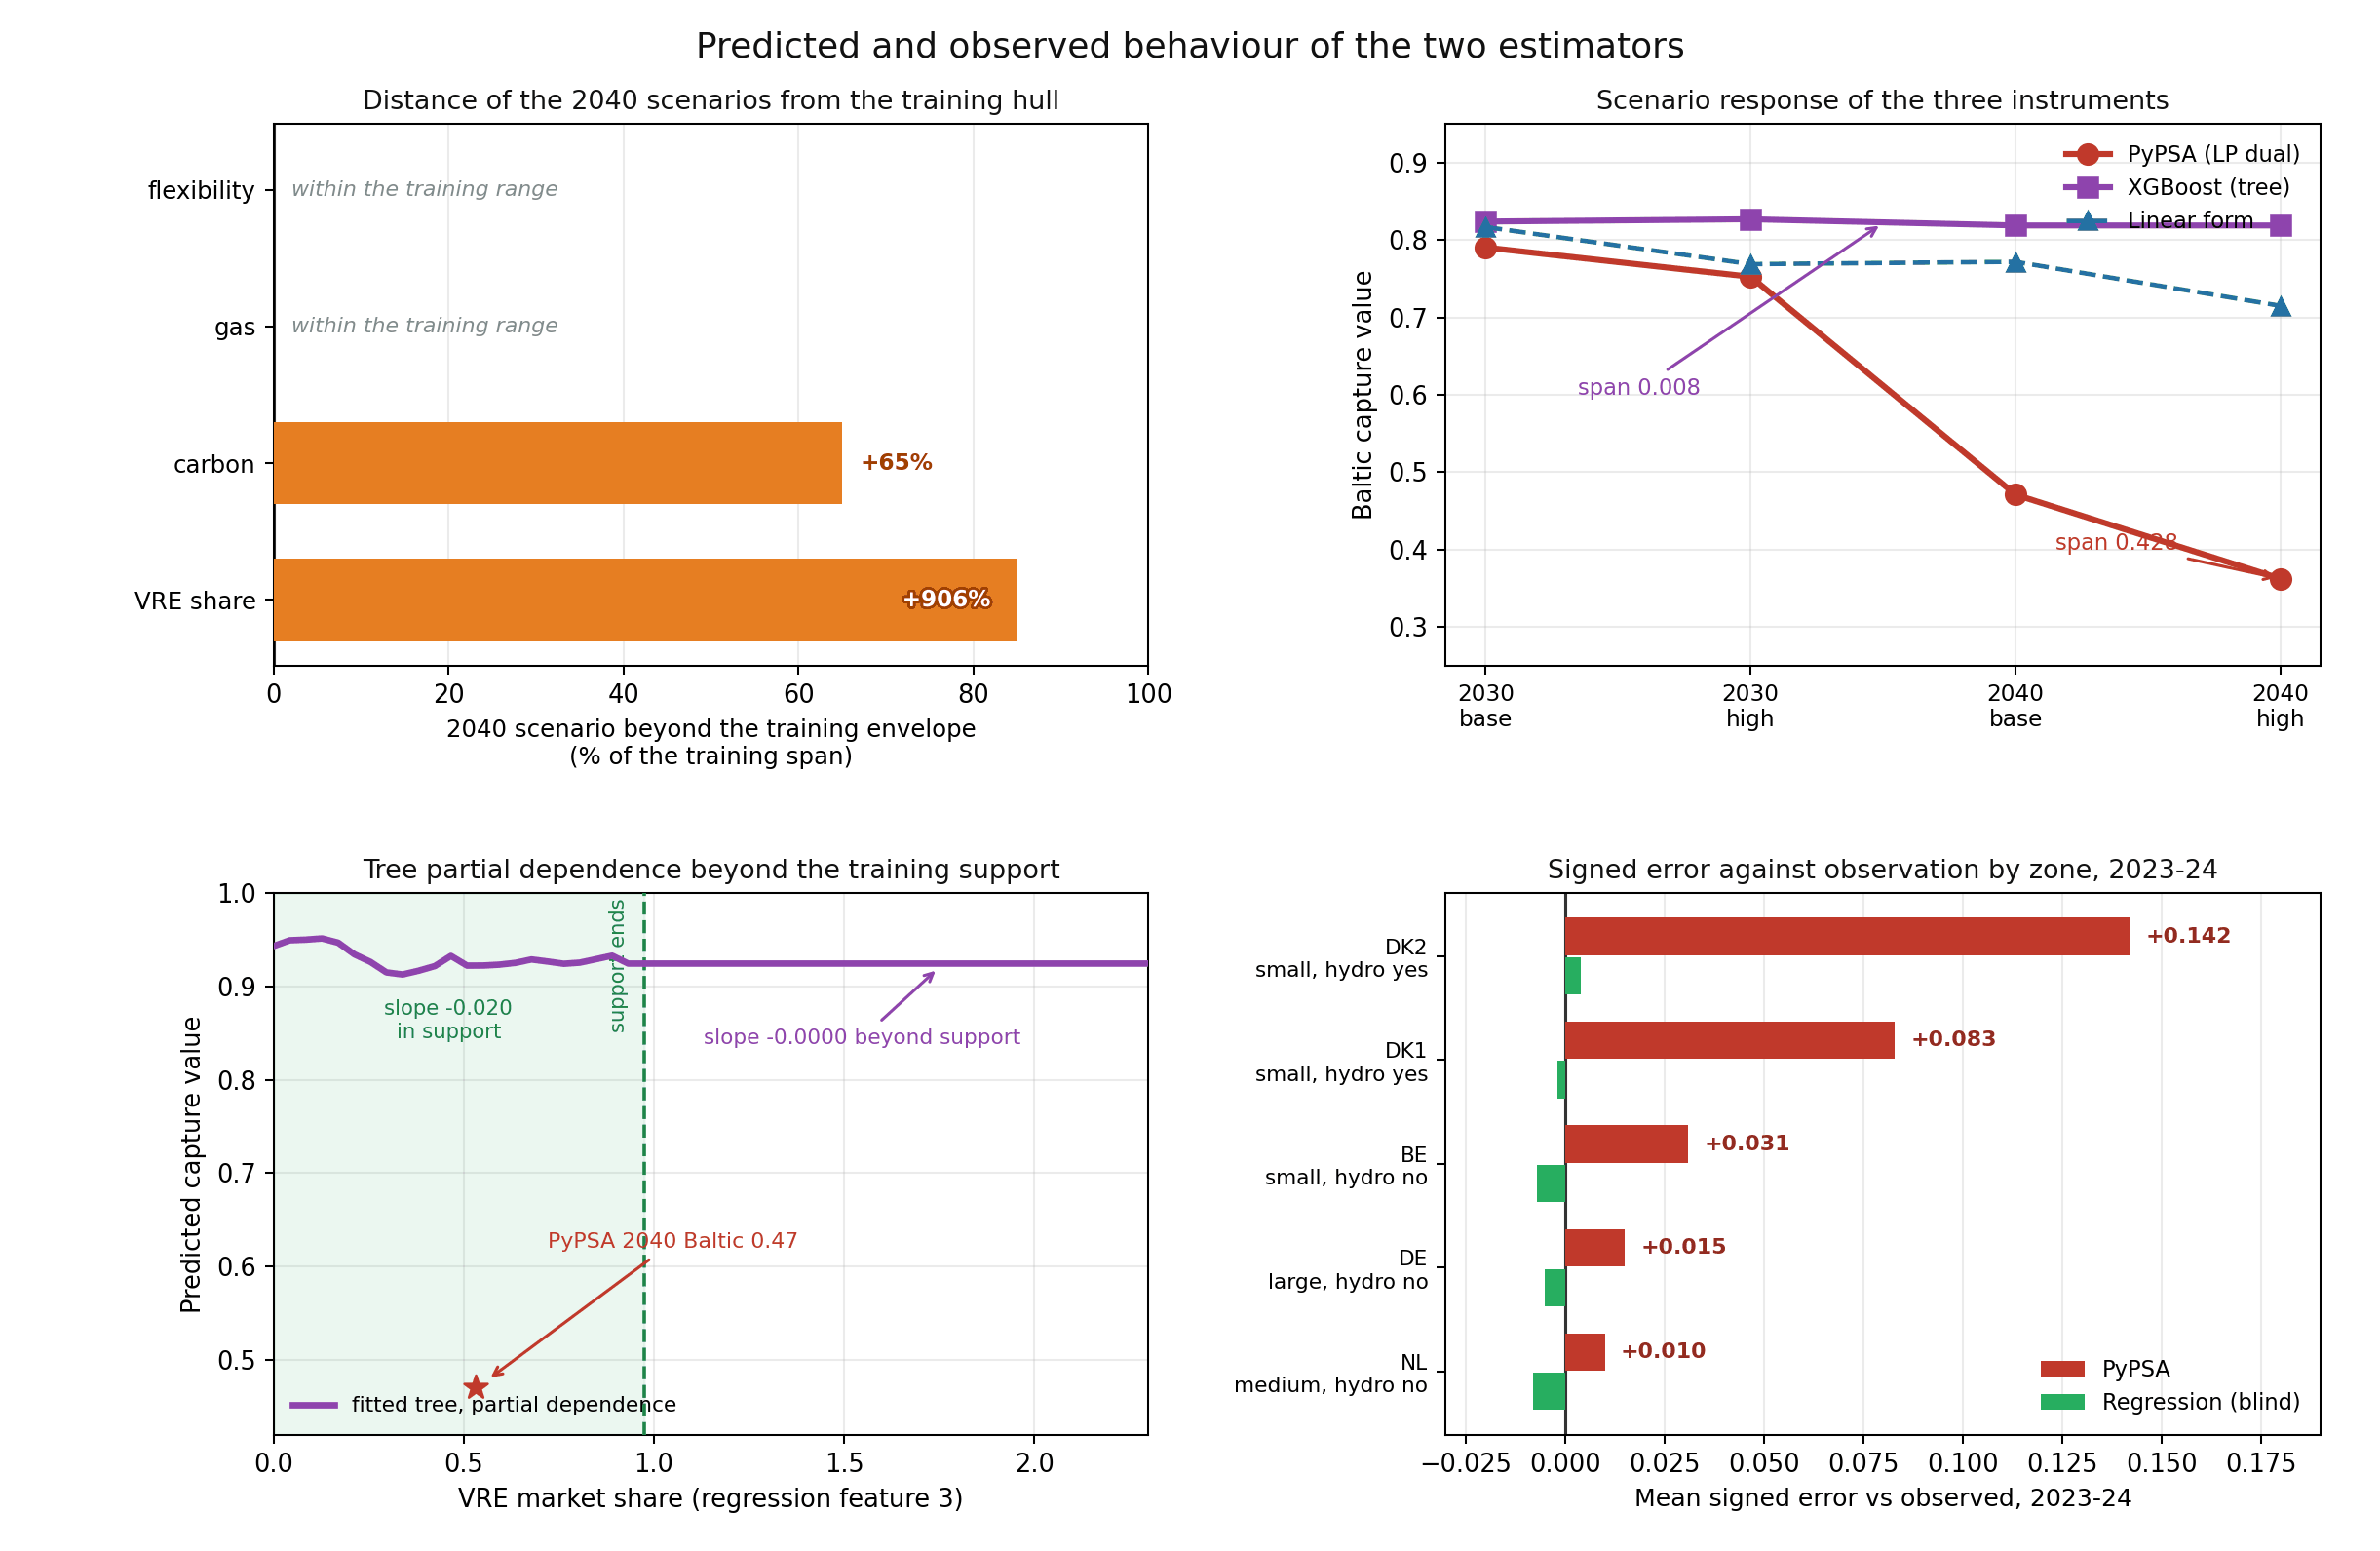
\includegraphics[width=0.95\textwidth]{fig_theory_vs_evidence}
    \caption{Why the models must differ, tested against the runs. Top
    left: every 2040 scenario leaves the training envelope, renewable share
    furthest. Top right: across the four Baltic scenarios the tree moves 0.008
    where the system model moves 0.43. Bottom left: the tree's fitted response
    is exactly flat beyond its support, so the divergence comes from leaving the range of the training data and does
    not reflect curvature. Bottom right: the system model's in-sample error is largest
    in small, hydro-coupled zones, the regression's is near zero, which fixes
    the sign and order of the bias correction.}
    \label{fig:theory}
\end{figure}

\begin{table}[!htb]
\centering\small
\caption{The two-estimator test in numbers. Response spans are across the four
Baltic 2040 scenarios; divergence is the mean absolute gap between the
models' Baltic estimates; curvature is the fast-approximation fit across 76 solved
networks with a cluster-bootstrap interval; errors are against observed
2023--24 capture values.}
\label{tab:theory_numbers}
\begin{tabular}{l >{\raggedright\arraybackslash}p{7.9cm}}
\toprule
Response span: tree / linear / analytical / system model & 0.008 / 0.102 / 0.179 / 0.428 \\
Divergence: in sample / 2030 / 2040 & 0.062 / 0.035 / 0.348 \\
Penetration-squared coefficient (95\,\% CI) & $-0.193$ [$-0.215$, $-0.169$]: concave \\
Mean signed error: system / regression & $+0.057$ / $-0.005$ \\
System error by zone & DK2 $+0.14$ > DK1 $+0.08$ > BE $+0.03$ > DE $+0.02$ > NL $+0.01$ \\
\bottomrule
\end{tabular}
\end{table}
\FloatBarrier

\FloatBarrier

\section{Portfolio and Distributional Analyses}\label{app:portfolio}

These analyses serve Objective~5 and the question of who bears the loss. They
are reported here in full; their conclusions are carried in
Sections~\ref{sec:site_ranking} and~\ref{sec:one_figure}.

\subsection{Spreading across both basins}\label{sec:diversification}

Objective~5 asks whether allocating capacity across both basins beats
concentrating it in the North Sea; the two channels of
Section~\ref{sec:mitigation} are tested separately because they give opposite
answers (Figure~\ref{fig:diversification}).

\begin{figure}[!htb]
    \centering
    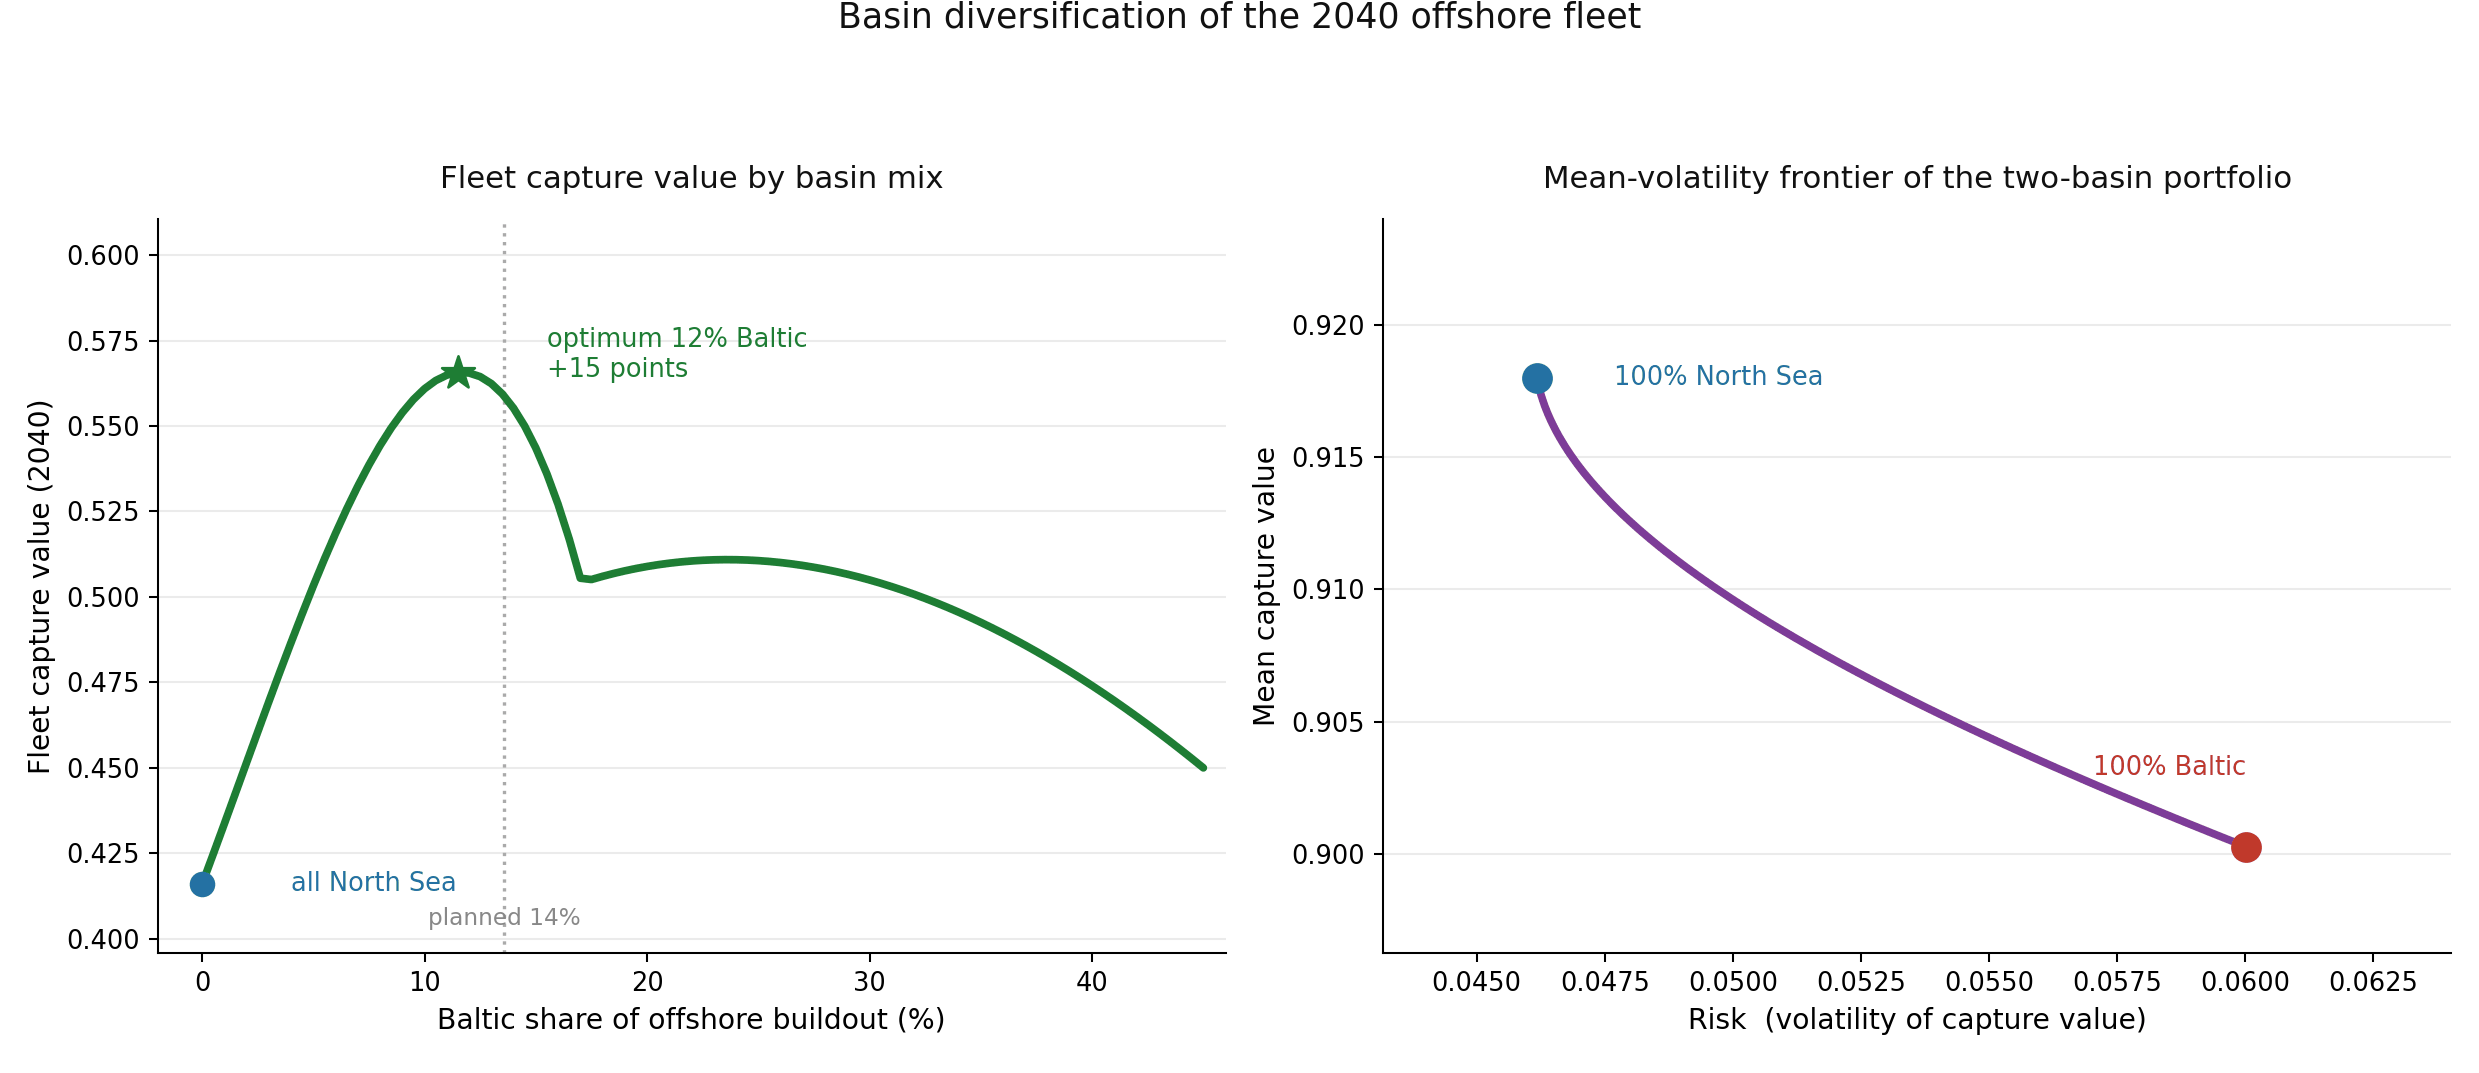
\includegraphics[width=0.94\textwidth]{fig_diversification}
    \caption{The two portfolio channels. Left: aggregate 2040 capture value of a
    fixed 623~TWh of offshore generation as a function of the share allocated to
    the Baltic, holding the total constant. Right: the mean-variance frontier
    built from monthly capture values, 2017 to 2024. Spreading the fleet raises
    the mean but does not reduce the variance.}
    \label{fig:diversification}
\end{figure}

The first channel is a cannibalisation hedge, and it works. Holding total
offshore generation fixed and varying only its split, an all-North-Sea
allocation cannibalises itself down to an aggregate capture value of 0.416,
while shifting 12\% to the Baltic, which starts earlier on its curve, lifts
the aggregate to 0.566, a gain of 36\%; the planned 14\% split is within
half a point of that optimum.

The second channel is a risk hedge, and it fails. Monthly capture values
over 2017 to 2024 make the North Sea simultaneously the higher-mean and
lower-variance basin (0.918 at 0.046 against 0.900 at 0.060), and the two
series co-move at a correlation of 0.80, so the minimum-variance portfolio
is 100\% North Sea and spreading delivers no volatility reduction at all.

The 0.28 wind correlation of Section~\ref{sec:mechanism} explains the split:
wind is decorrelated, so moving capacity eases cannibalisation, but market
coupling propagates price levels across borders. The benefit of spreading
sits entirely in the mean: the portfolio is less cannibalised, while its
volatility barely changes.

% ----------------------------------------------------------------------------
\subsection{Method: decomposing capture value by price state and pricing congestion rent}\label{app:whopays_method}

\subsubsection*{Who bears the loss: decomposing capture value by price
level}\label{sec:whopays_method}

A capture value states how much revenue is lost. It does not state who loses it,
and under the support instruments reviewed in
Section~\ref{sec:mitigation} the answer differs by mechanism. A two-sided
contract for difference tops any positive price up to the strike, and volumes
constrained off by the network are compensated under Article~13 of Regulation
(EU) 2019/943 \cite{EURegulation2019943}, so both losses fall on the state. In a
zero or negative price hour the contract is suspended, following GB practice from
allocation round four and the 2024 market design reform
\cite{EUMarketReform2024}, so that loss falls on the farm and no compliant
scheme may cover it. What decides the bearer is therefore the price \emph{level},
not the physical cause.

Capture value factorises to match. Writing $z$ for the share of generation
occurring in hours priced below a threshold $\epsilon$, and $\mathrm{CV}^{+}$ for
the capture value computed over the remaining hours,
%
\begin{equation}
    \mathrm{CV} = (1 - z)\,\mathrm{CV}^{+},
    \qquad\text{so}\qquad
    \underbrace{1 - \mathrm{CV}}_{\text{total loss}}
    = \underbrace{z}_{\text{farm-borne}}
    + \underbrace{(1-z)\bigl(1 - \mathrm{CV}^{+}\bigr)}_{\text{state-borne}}
    \label{eq:whopays}
\end{equation}
%
and the split is exact, with nothing left over. The farm-borne term is energy earning
nothing with the contract suspended; the state-borne term is the depression of
positive prices that the contract absorbs. Both are computed hour by hour on the solved networks for
2030 and 2040 under the frozen and cost-optimal grids, with
$\epsilon = 1$~\euro/MWh. Because the linear program floors prices at zero
(Section~\ref{sec:pypsa_how}), $z$ is a conservative lower bound on the real
farm-borne share, which in a market with a negative-price tail would be larger.
Curtailed volume is reported separately, since it never enters capture value at
all yet is compensated under the same Article~13. The observed anchor is the
wind-weighted share of 2023 and 2024 generation falling in hours with a
day-ahead price at or below zero. A required strike price, $\mathrm{LCOE}/(1-z)$,
follows directly and states what a contract must pay if the farm is to recover
its costs given that a share $z$ of its output earns nothing.

\subsubsection*{Congestion rent and who funds the
remedy}\label{sec:rent_method}

If interconnection is the lever, its affordability is a fair question, and the
income that congestion itself generates is the natural place to look. For every
branch the rent is the flow multiplied by the price difference across it, summed
over the year:
%
\begin{equation}
    R_{\ell} = \sum_{t} w_t \, f_{\ell,t}
    \bigl( \eta_{\ell}\,\lambda_{\mathrm{to}(\ell),t} - \lambda_{\mathrm{from}(\ell),t} \bigr)
    \label{eq:congestion_rent}
\end{equation}
%
with $f_{\ell,t}$ the flow, $\lambda$ the nodal prices, $w_t$ the snapshot
weighting, and $\eta_{\ell}$ the efficiency, which is unity for lossless lines
and the link efficiency for controllable interconnectors. Rents are aggregated by
border and classified by whether each branch is internal to a basin or crosses
its boundary. The same quantity is computed on the frozen and the cost-optimal
network, so that the difference measures the rent that building the grid
destroys, which is the merchant-transmission problem Joskow and Tirole
\cite{JoskowTirole2005} identify. Against that income sits the annualised capital cost of the transmission the optimal solve builds, taken as the added
capacity multiplied by its annuitised cost. Because frozen-grid Poland prices
several hundred scarcity hours, every rent figure is reported twice, once over
all hours and once excluding hours above 390~\euro/MWh, the same threshold used
for the scarcity sensitivity in Section~\ref{sec:scarcity_method}. The comparison must not be added to the captured-revenue gain of
Section~\ref{sec:vlcoe_grid_method}: both arise from the same price convergence,
and building the lines removes the rent, so the two must not be summed.

\subsection{Who bears the loss, and what funds the cure}\label{sec:whopays_results}

Every number so far has said how much value is lost; who loses it is a
separate question with a different answer. Applying the factorisation of Equation~\ref{eq:whopays} splits
each basin's erosion into the part a contract absorbs and the part it cannot;
Figure~\ref{fig:whopays} draws that split for both basins and both grids.

\begin{figure}[!htb]
    \centering
    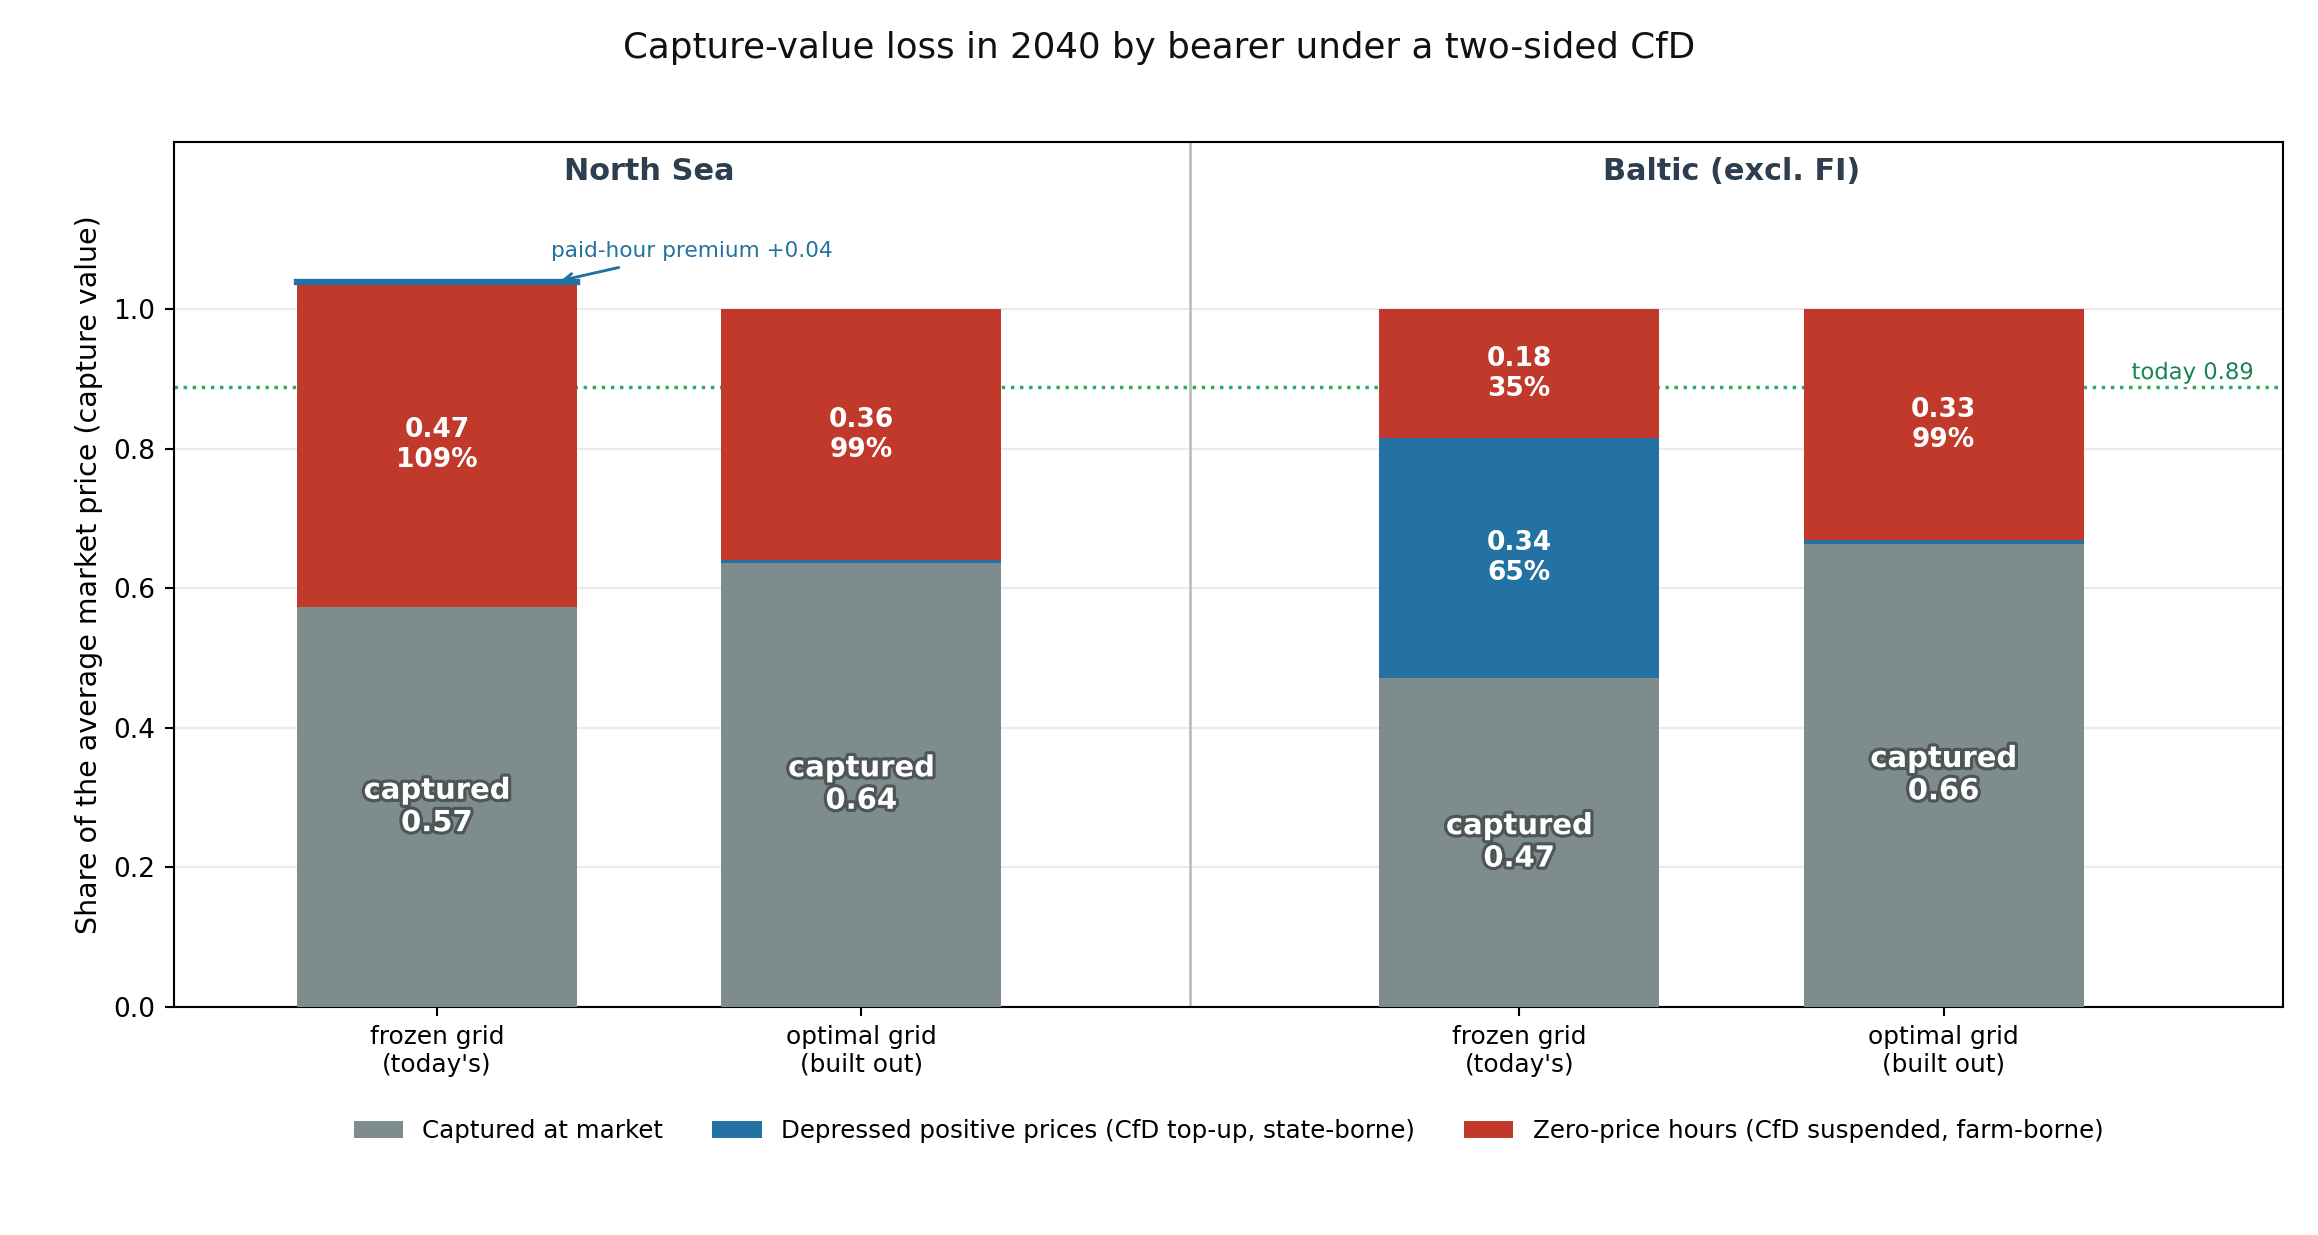
\includegraphics[width=0.94\textwidth]{fig_whopays_decomposition}
    \caption{The 2040 capture-value loss split by bearer. The grey block is
    revenue captured at market. The blue block is value lost to depressed but
    positive prices, which a two-sided contract tops up to the strike, so the
    state carries it. The red block is energy earning nothing, where the contract
    is suspended and the farm carries it. In the frozen North Sea the paid hours
    earn a small premium ($+0.04$), which offsets part of the zero-price loss,
    so the farm-borne share amounts to 109\% of the net loss.}
    \label{fig:whopays}
\end{figure}

The two basins look similar on the capture-value chart and are opposites
underneath it. The frozen-grid Baltic factorises as
$(1-z)\,\mathrm{CV}^{+} = 0.815 \times 0.578$:
only 18.5\% of its energy earns nothing, so almost two-thirds of its loss is
depressed-but-paid, the kind a contract absorbs. The North Sea factorises as
$0.533 \times 1.075$: its paid hours earn slightly above average, so there is
no depression to top up and the entire loss is uncompensable; with
$\mathrm{CV}^{+}$ above one the state term is a small premium, so the farm's share slightly exceeds the loss itself. The basin with the worse
headline number has the better protected investor.

Volume shows the same split from the other side: the frozen-grid North Sea
spills a third of its available 2040 energy against 3.6\% in the Baltic,
curtailment being a further state-borne bill invisible to capture value.

Building the grid does not simply reduce the loss, it changes its bearer.
Under optimal expansion the depression factor snaps to about 0.99 in both
basins, so what survives is purely the zero-price channel: the share of Baltic
energy earning nothing \emph{rises} from 18.5\% to 33.1\% even as capture
value improves, because interconnection couples the basin to the wider
system's surplus hours, and roughly 99\% of the remaining loss becomes
farm-borne: a fiscal problem converted into an investor one, a consequence
absent from the transmission-benefit literature.

The zonal detail separates three regimes the basin averages hide
(Appendix~\ref{app:tables}): scarcity-priced Poland, the locally oversupplied
eastern Baltic, and the open North Sea, most exposed but most relieved. The
strike a contract needs follows the same split, $\mathrm{LCOE}/(1-z)$,
roughly 71~\euro/MWh for Poland against 125 to 210 across the open zones,
converging to 92 to 103 under expansion: an ordering that inverts the
capture-value ranking for a contract-backed investor.

All farm-borne shares here are conservative: the linear program floors prices
at zero, and the observed 2023 to 2024 anchors already show 5.9\% of North
Sea and 3.0\% of Baltic generation at or below zero, so the real exposure is
larger than reported.

% ----------------------------------------------------------------------------
\subsubsection{Congestion rent and the cost of the cure}\label{sec:rent_results}

The recommendation that follows is to build transmission, and its
affordability need not be a public spending question: congestion is itself a
revenue stream, and Article~19 of Regulation (EU) 2019/943 already earmarks
that revenue for this purpose \cite{EURegulation2019943}.
Equation~\ref{eq:congestion_rent} prices it. The rent accrues to the transmission operators, and none of it reaches
generators: congestion is only ever a cost to a wind farm, and the question here is only whether the
system's own congestion income covers the cure.

\begin{table}[!htb]
\centering
\small
\caption{Annual congestion rent in 2040, in billion euro per year, computed on
the frozen and cost-optimal networks. Figures are given over all hours and
excluding scarcity hours above 390~\euro/MWh, since frozen-grid Poland prices
several hundred such hours. The grid cost is the annualised capital cost of all
transmission the cost-optimal solve builds across the fourteen countries.}
\label{tab:congestion_rent}
\begin{tabular}{l r r}
\toprule
 & \textbf{All hours} & \textbf{Excluding scarcity} \\
 & (bn\euro{} per year) & (bn\euro{} per year) \\
\midrule
System congestion rent, frozen grid & 38.9 & 22.6 \\
\quad of which Baltic-related & 11.8 & 4.3 \\
System congestion rent, optimal grid & 15.2 & 15.1 \\
\quad of which Baltic-related & 2.1 & 2.1 \\
\midrule
Rent destroyed by building the grid & 23.7 & 7.4 \\
Annualised capital cost of the new lines & 2.7 & 2.7 \\
\midrule
\textbf{Baltic rent as a multiple of total grid cost} & \textbf{4.4$\times$} & \textbf{1.6$\times$} \\
\bottomrule
\end{tabular}
\end{table}

The conservative column is the one to quote: even excluding every scarcity
hour, Baltic-related borders generate 4.3~bn\euro{} per year against an
annualised 2.7~bn\euro{} for the entire fourteen-country expansion. The
enclosed basin already produces, and by statute already earmarks, more than
enough income to pay for the interconnection that would relieve it, and the
concentration is specific: the German-Polish border alone carries
7.2~bn\euro{} on the frozen grid. Poland's borders are where the money and
the constraint coincide.

Two qualifications matter. First, the rent and the captured-revenue gain
must not be added: building the lines destroys the rent that funds them, the
merchant transmission problem in its original form \cite{JoskowTirole2005},
so the rent is the pre-existing, ring-fenced funding pool and the welfare
gain the justification. Second, expansion is not congestion-free: Baltic
\emph{border} rent collapses from 2.9 to 0.7~bn\euro{} while \emph{internal}
rent barely moves, so interconnection resolves the enclosure and leaves the
domestic bottlenecks standing.

% ----------------------------------------------------------------------------

\section{Forecast Checks on the Two Models}\label{app:forecast_checks}

Each model's mean squared error is separated following Theil \cite{Theil1966}:
\begin{equation}
\mathrm{MSE} = \underbrace{(\bar{\hat y}-\bar{y})^{2}}_{\text{bias}}
+ \underbrace{(s_{\hat y}-s_{y})^{2}}_{\text{variance}}
+ \underbrace{2(1-r)\,s_{\hat y}s_{y}}_{\text{covariance}},
\label{eq:theil}
\end{equation}
whose three shares sum to one.


Section~\ref{sec:backtest} states the conclusions of two checks on the models
as forecasters. This appendix carries them in full.

\subsection{Backtesting the act of projecting}

Skill on held-out targets tests the models but not the projection, which
additionally has to build its future inputs. The one horizon where that whole
chain can be scored is the recent past: fitted on data to 2021 and asked for
2023 and 2024, across the same four zones, ninety-six zone-months
(Table~\ref{tab:backtest}).

Three results follow. The first is that building the feature vectors costs
nothing. Predicting from constructed inputs, with the weather terms at each
farm's pre-2022 monthly climatology and the system terms carrying the pre-2022
monthly shape, is not worse than predicting from the realised features but
slightly better, 0.049 against 0.053. The seasonal construction smooths
month-to-month movements the model could not have anticipated in any case, so
it acts as a mild regulariser. Whatever is wrong with the projection at 2040, it is not the construction of the inputs.

The second is that over this horizon the two approaches project equally well.
The constructed-input regression and the system model both score 0.049. Both
over-predict, by 0.019 and 0.041, which is cannibalisation deepening faster than
either anticipated, and the system model is again the more bias-dominated of the
two, at 0.33 of squared error against 0.09.

The third explains the first two and connects them to the projection proper.
This backtest is only a mild excursion beyond the training data. Of the 2023--24
observations, 58\,\% lie inside the pre-2022 range on all seven features at
once, and the single feature breached at any scale is the carbon price, at
42\,\% of rows, which Section~\ref{sec:gap_decomposition} showed to be inert.
The regression model still largely holds support here, and where it holds
support it projects as well as the system model does. That is the finding: the
divergence at 2040 is not a general difference in forecasting ability between
the two model families, since over a two-year horizon inside the data there is
no such difference. It is specific to the loss of support, where 2040 leaves
every one of the thirty-six projection rows outside the joint training range
rather than 42\,\% outside on one inert feature.

\begin{table}[!htb]
\centering\small
\caption{Backtest of the projection: fitted on data to 2021, scored on 96
zone-months in 2023 and 2024. Shares are the Theil partition and sum to one.
The constructed inputs use realised annual levels, so the test grants perfect
scenario foresight.}
\label{tab:backtest}
\begin{tabular}{l c c c c c c}
\toprule
& & & & \multicolumn{3}{c}{\textbf{Share of squared error}} \\
\cmidrule(lr){5-7}
\textbf{Prediction} & \textbf{MAE} & \textbf{RMSE} & \textbf{Bias} &
\textbf{Bias} & \textbf{Var.} & \textbf{Cov.} \\
\midrule
Regression, realised features  & 0.053 & 0.066 & $+0.027$ & 0.17 & 0.12 & 0.72 \\
Regression, projected features & 0.049 & 0.063 & $+0.019$ & 0.09 & 0.33 & 0.58 \\
System model                   & 0.049 & 0.071 & $+0.041$ & 0.33 & 0.16 & 0.51 \\
\bottomrule
\end{tabular}
\end{table}

\begin{figure}[!htb]
    \centering
    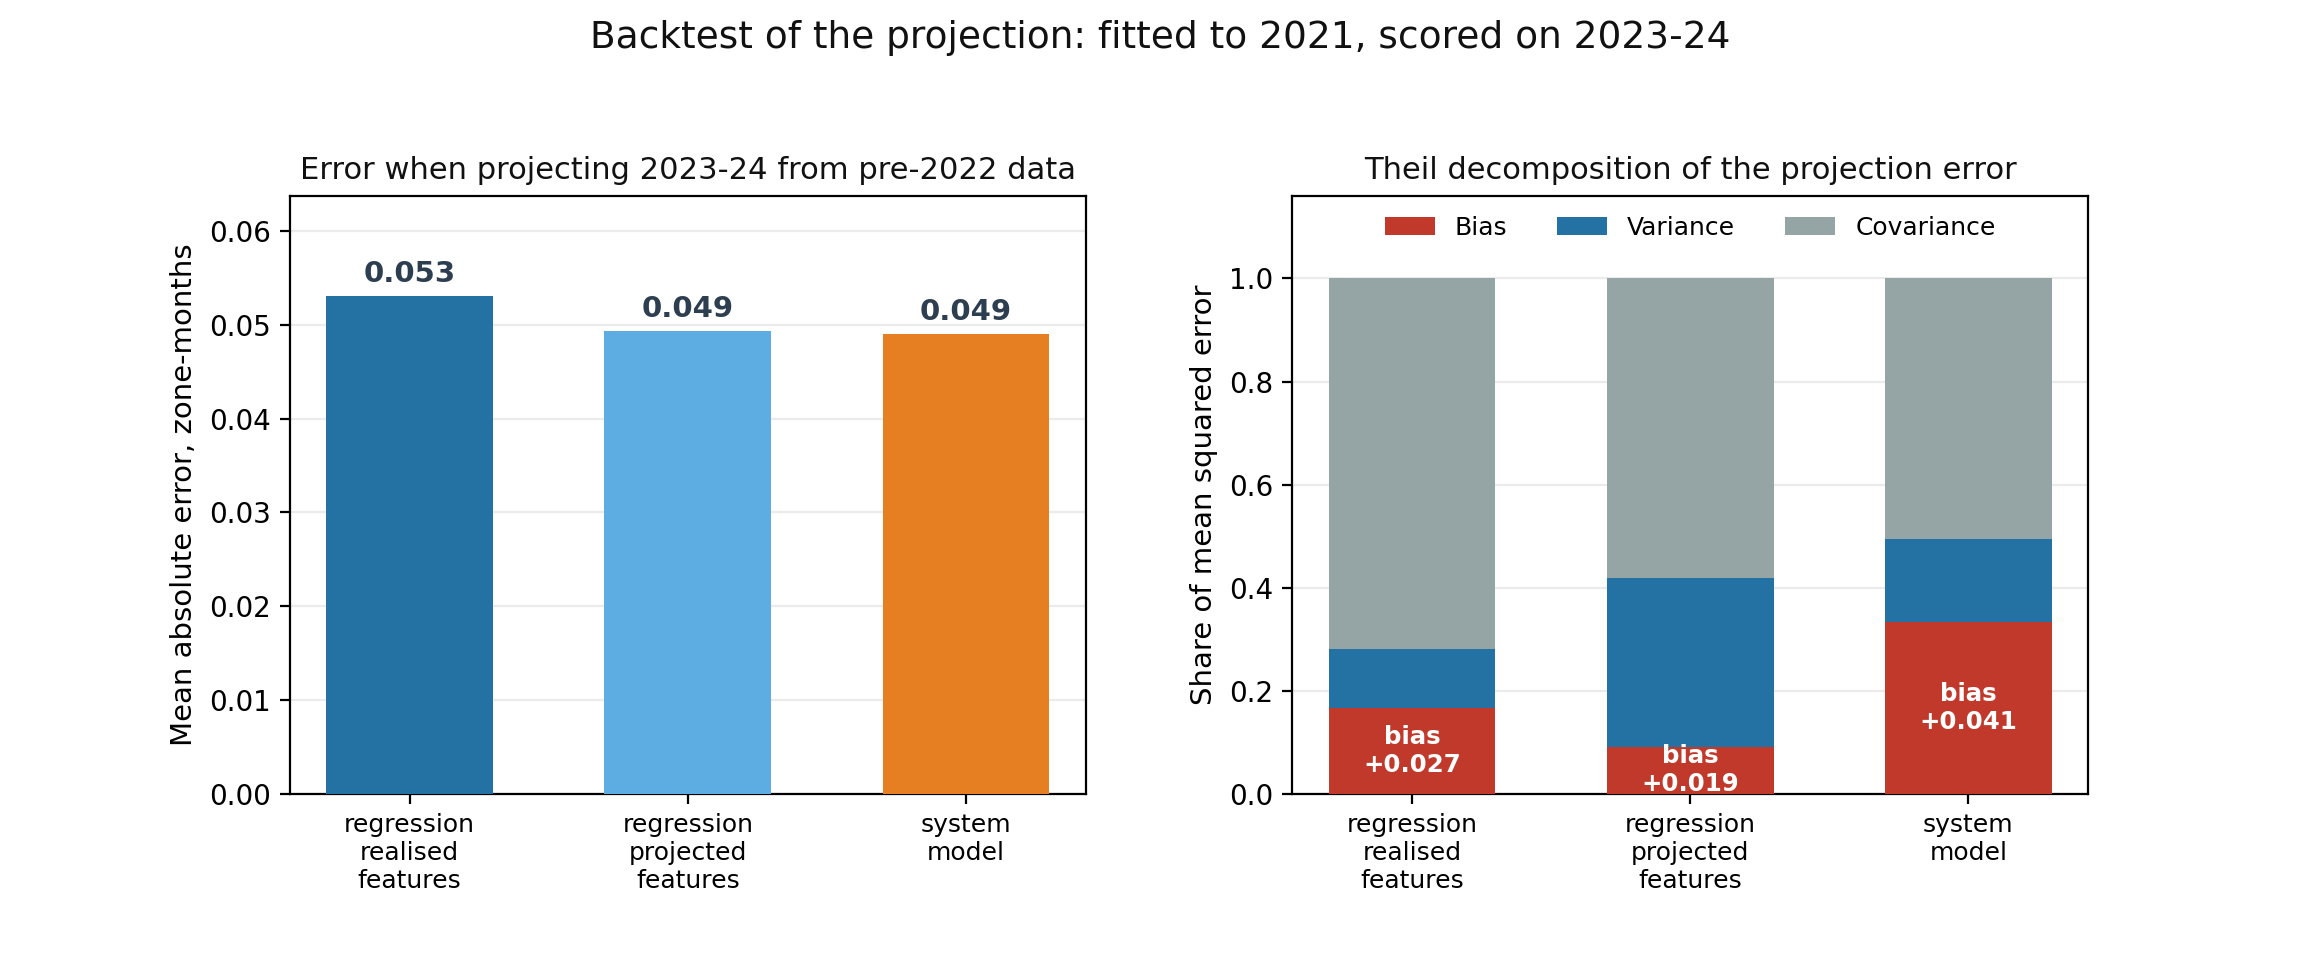
\includegraphics[width=0.92\textwidth]{fig_projection_backtest}
    \caption{Backtesting the projection. Left: error when each approach is
    fitted to 2021 and asked for 2023 and 2024; constructing the input vectors
    costs nothing, and the constructed-input regression matches the system
    model. Right: the Theil partition, where the system model remains the more
    bias-dominated of the two.}
    \label{fig:backtest}
\end{figure}
\FloatBarrier

\subsection{The two projections against external evidence}

Neither model can be scored at 2040, because 2040 has no observations. But the
projections are not therefore unfalsifiable, because the published literature
carries expectations against which both can be placed
(Table~\ref{tab:external}). Running the regression model forward exactly as its
predecessor does, building twelve monthly feature vectors per horizon from the
scenario levels and the farm's own seasonal shape, it returns a Baltic 2040
band of 0.72 to 0.85 with no farm inside the training range. The system model
returns 0.36 to 0.60, centrally 0.47.

Read naively, this favours the regression model. Its band sits inside the
published range and brackets Germany's measured 0.76 almost exactly, while the
system model falls below every benchmark. The reading inverts once the
penetrations at which those benchmarks were measured are attached to them.
Hirth's band is estimated at a 30\,\% share and Germany's 0.76 at 35\,\%, both
comfortably inside the regression model's training range. A model that cannot
leave the regime it was fitted on will land among benchmarks drawn from that
same regime whether or not it is right about 2040, so the agreement is not
corroboration. It is the constant response of Section~\ref{sec:gap_decomposition} producing
a plausible number.

The benchmark that discriminates is the one measured in a market that is
already saturated. Aurora's French offshore holds near 0.94 to 2060, which is
an under-built market and the analogue of the Baltic today rather than the
Baltic of 2040; its French solar, heavily built out, falls to about 0.59 and
stays there \cite{Aurora2025_France}. That is the closest available analogue to
what the Baltic becomes, and it lies inside the system model's raw range and
above the regression model's band. The comparison is developed further in
Section~\ref{sec:disc_literature}.

The decisive quantity, however, is neither estimate. Between a baseline Baltic
buildout and a high one, the regression model's answer moves by 0.008 while the
system model's moves by 0.428. A projection that barely changes between two
different futures is not a forecast of the buildout, however reasonable its
value looks beside the literature. This is what the constant response means in practice, and it is the reason
the external evidence confirms the allocation of roles rather than
establishing it.

\begin{table}[!htb]
\centering\small
\caption{The two projections for the Baltic in 2040, against published
benchmarks. The penetration column is what makes the comparison work: every
benchmark below the rule was measured inside the regression model's training
range, and only the last was measured in a saturated market.}
\label{tab:external}
\begin{tabular}{l c l}
\toprule
\textbf{Source} & \textbf{Capture value} & \textbf{Measured at} \\
\midrule
Regression model, 2040 Baltic & 0.72--0.85 & no farm inside training range \\
System model, 2040 Baltic & 0.36--0.60 (central 0.47) & projected buildout \\
\midrule
Hirth \cite{Hirth2013} & 0.5--0.8 & 30\,\% share \\
Germany \cite{Stiewe2025, Ember2025} & 0.76 & 35\,\% share \\
Jacquet, worst North Sea case \cite{Jacquet2024} & $\approx 0.6$ & North Sea buildout \\
Aurora, French offshore \cite{Aurora2025_France} & $\approx 0.94$ & under-built market \\
\midrule
Aurora, French solar \cite{Aurora2025_France} & $\approx 0.59$ & \textbf{saturated market} \\
\bottomrule
\end{tabular}
\end{table}
\FloatBarrier



\section{The Analytical Equation}\label{app:analytical}

Section~\ref{sec:one_equation} states the conclusion of the per-basin
analytical fit. This appendix carries it in full.

\subsection{One equation, two basins}

SHAP names the influential features; the analytical equation describes the
mechanism's shape in closed form. Refit per basin, the same equation fits both
seas and answers the second research question in its sharpest form: the
pattern-penalty exponent is 0.74 in
the Baltic against 0.37 in the North Sea, steeper in 99 of 100 farm-block
bootstraps (Figure~\ref{fig:constants}). The absolute fit is low by design,
fitted for interpretable shape rather than prediction, so the load-bearing
result is the bootstrap-stable gap. Since the exponent trades off against the
penalty's scale, the fair summary is the implied slope of capture value against
penetration at common conditions: about 1.6 times the North Sea's today and 1.9
times at the dominance a buildout creates. On a fifteen-farm panel that is
directional rather than definitive, but it is consistent with the system model's
moderate-2030, severe-2040 trajectory
(Section~\ref{sec:projection_results}).


\section{Regression Validation and Earlier-Horizon Maps}\label{app:reg_tables}

Supporting Sections~\ref{sec:trust} and~\ref{sec:maps}; the numbers are quoted
in the body.

\begin{table}[!htb]
\centering
\small
\caption{The five algorithm families, out-of-sample $R^2$ on the bidding-zone panel, untuned. Random K-fold withholds farm-months; leave-farm-out withholds whole farms, so it scores entirely unseen sites, where the polynomial's squared and cross terms explode.}
\label{tab:algorithms}
\begin{tabular}{l c c}
\toprule
\textbf{Algorithm} & \textbf{Random K-fold} & \textbf{Leave-farm-out (strict)} \\
\midrule
Gradient boosting (XGBoost) & 0.752 & \textbf{0.686} \\
Random forest & 0.682 & 0.636 \\
Support-vector regression & 0.583 & 0.497 \\
Linear (OLS) & 0.330 & 0.270 \\
Polynomial (degree~2) & 0.437 & $-19.9$ \\
\bottomrule
\end{tabular}
\end{table}

\begin{table}[!htb]
\centering
\small
\caption[Out-of-sample $R^2$ of the gradient-boosting model per scheme]{Out-of-sample $R^2$ of the untuned gradient-boosting model under each
scheme, at country versus bidding-zone resolution. Both K-fold rows are scored
out-of-fold and differ only in what they withhold: random farm-months (leaky,
for comparability with Jacquet's untuned 0.82 \cite{Jacquet2024}) versus whole farms
(strict).}
\label{tab:regression_metrics}
\begin{tabular}{l c c}
\toprule
\textbf{Validation scheme} & \textbf{Country features} & \textbf{Zone features} \\
\midrule
Random K-fold (comparability) & 0.733 & 0.752 \\
Leave-farm-out (headline) & 0.598 & \textbf{0.686} \\
Leave-farm-out, excluding 2022 & 0.607 & 0.692 \\
North Sea $\rightarrow$ Baltic transfer & 0.360 & 0.379 \\
Time split (train $\leq$2022, test 2023--24) & $-0.093$ & $-0.032$ \\
\bottomrule
\end{tabular}
\end{table}

\begin{figure}[!htb]
    \centering
    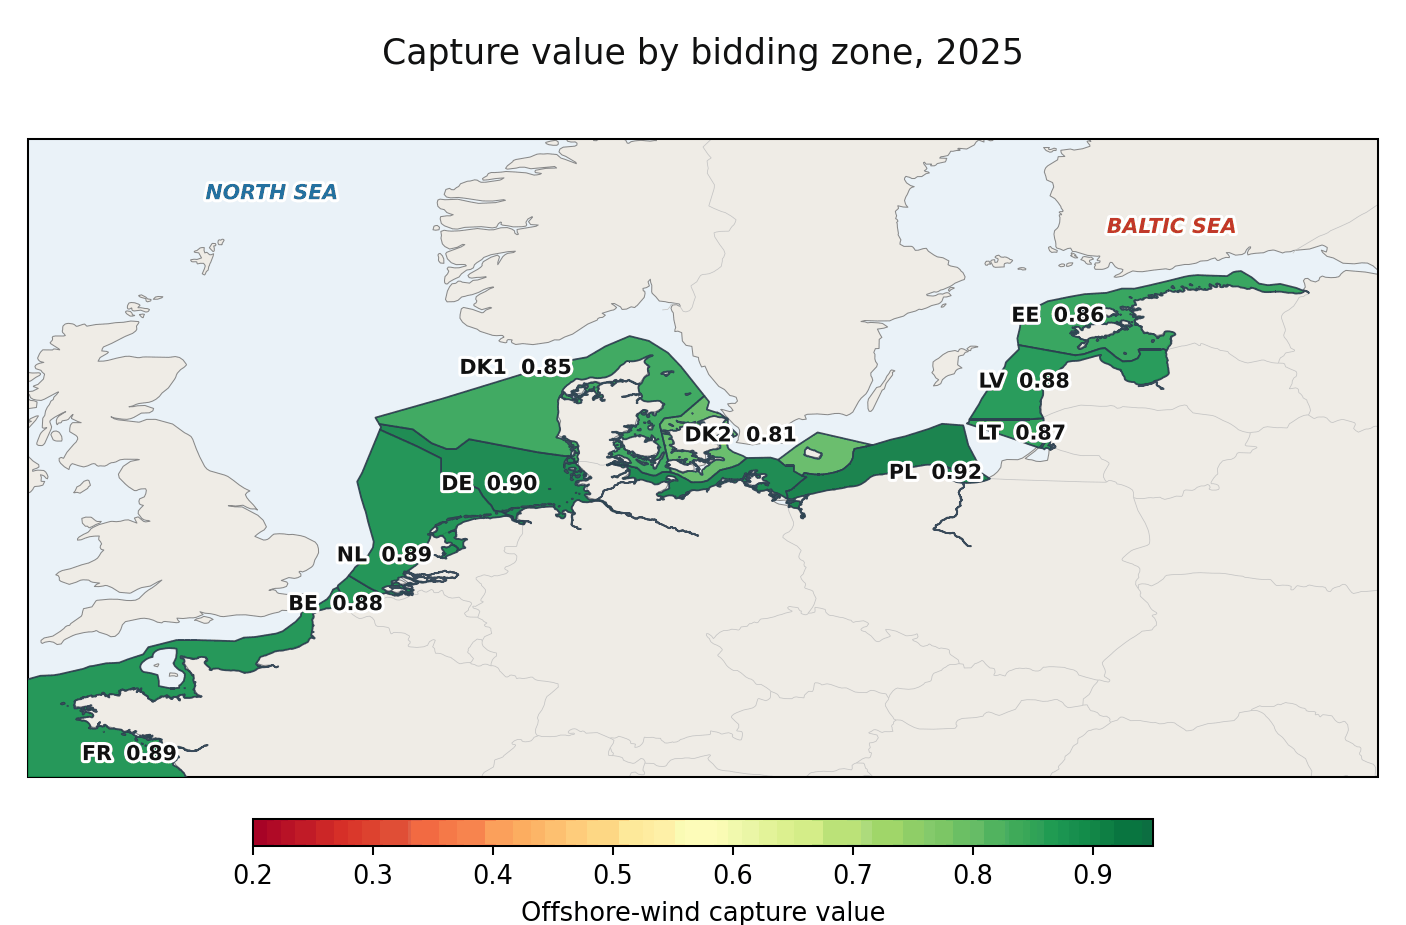
\includegraphics[width=0.80\textwidth]{fig_heatmap_2025}
    \caption{Offshore capture value across both shelves, 2025. Capture value is high and nearly uniform across both shelves: the under-built
    Baltic sits level with the North Sea, and
    the theoretical Baltic premium is not visible.}
    \label{fig:heatmap_2025}
\end{figure}

\begin{figure}[!htb]
    \centering
    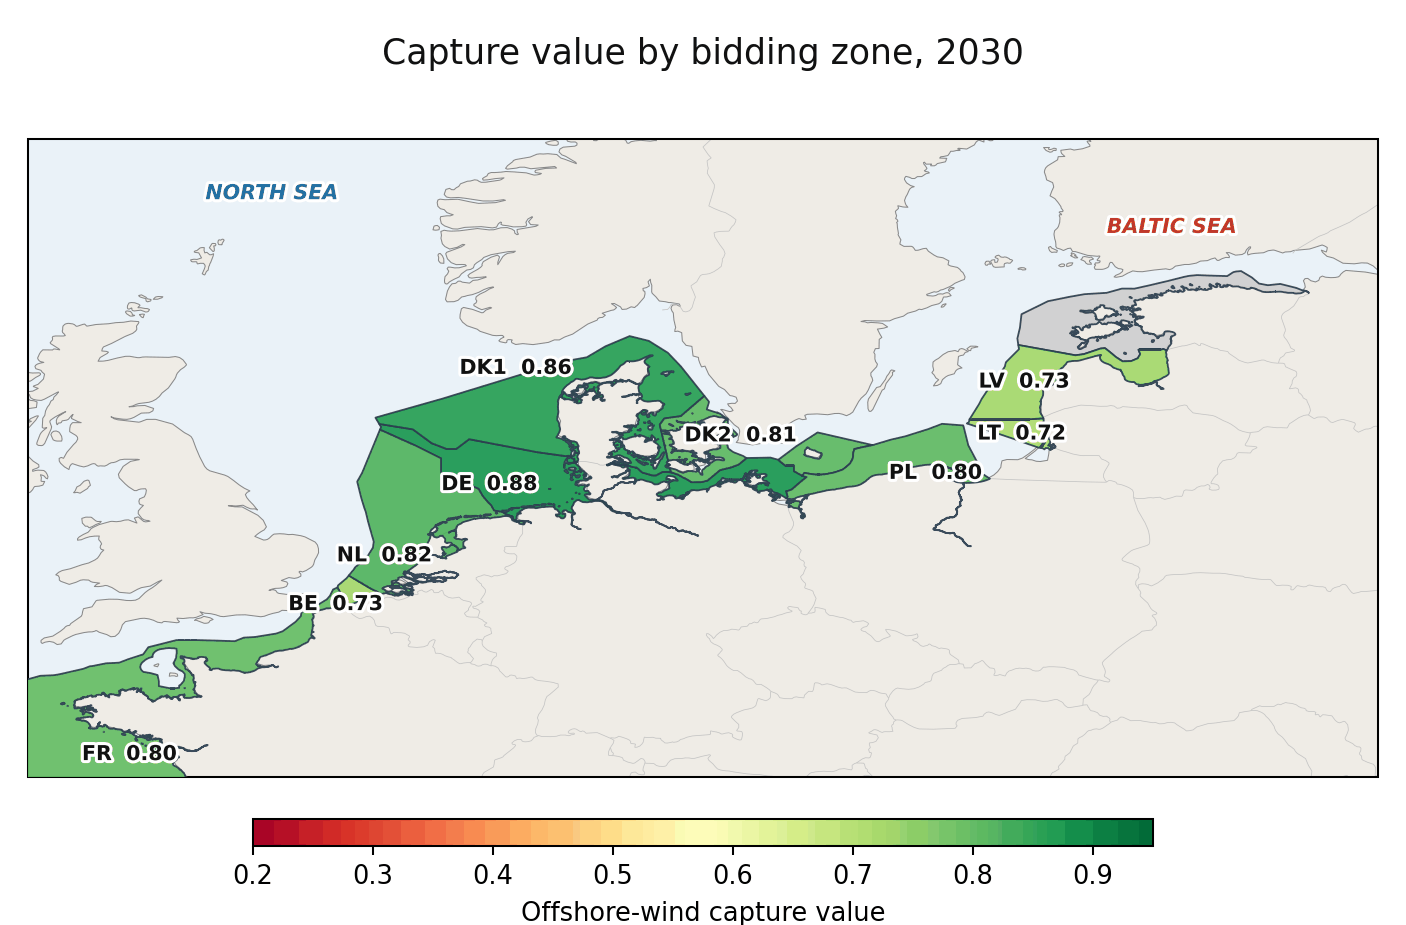
\includegraphics[width=0.80\textwidth]{fig_heatmap_2030}
    \caption{The same field in 2030. The first tranche of the buildout is in place. Values have fallen slightly
    and remain high in both basins, with the Baltic beginning to fall further
    as its own correlated output crowds its price.}
    \label{fig:heatmap_2030}
\end{figure}
\section{Model Comparison Against Observed Prices: Full Detail}\label{app:triangle}

The per-zone-year detail behind Sections~\ref{sec:trust}
and~\ref{sec:why_differ}; the aggregates are quoted in the body.

\begin{table}[!htb]
\centering\small
\caption{The three-way comparison in numbers: observed capture value against
each model's estimate, with signed errors, for all fifteen zone-years. The
regression column is out of fold, from a model that never trained on the
zone's farms.}
\label{tab:triangle}
\begin{tabular}{l l c c c r r}
\toprule
\textbf{Zone} & \textbf{Year} & \textbf{Observed} & \textbf{Regression} &
\textbf{System model} & \textbf{Reg.\ error} & \textbf{Sys.\ error} \\
\midrule
DE  & 2019 & 0.923 & 0.948 & 0.984 & $+0.025$ & $+0.061$ \\
NL  & 2019 & 0.977 & 0.967 & 0.986 & $-0.010$ & $+0.009$ \\
BE  & 2019 & 0.919 & 0.925 & 0.983 & $+0.006$ & $+0.064$ \\
DK1 & 2019 & 0.924 & 0.929 & 0.986 & $+0.005$ & $+0.062$ \\
DK2 & 2019 & 0.933 & 0.936 & 0.987 & $+0.003$ & $+0.054$ \\
\addlinespace
DE  & 2023 & 0.909 & 0.913 & 0.908 & $+0.004$ & $-0.001$ \\
NL  & 2023 & 0.881 & 0.887 & 0.883 & $+0.006$ & $+0.002$ \\
BE  & 2023 & 0.869 & 0.879 & 0.896 & $+0.010$ & $+0.027$ \\
DK1 & 2023 & 0.854 & 0.861 & 0.917 & $+0.007$ & $+0.063$ \\
DK2 & 2023 & 0.784 & 0.798 & 0.927 & $+0.014$ & $+0.143$ \\
\addlinespace
DE  & 2024 & 0.910 & 0.896 & 0.941 & $-0.014$ & $+0.031$ \\
NL  & 2024 & 0.900 & 0.878 & 0.919 & $-0.022$ & $+0.019$ \\
BE  & 2024 & 0.893 & 0.869 & 0.928 & $-0.024$ & $+0.035$ \\
DK1 & 2024 & 0.843 & 0.833 & 0.947 & $-0.010$ & $+0.104$ \\
DK2 & 2024 & 0.808 & 0.802 & 0.949 & $-0.006$ & $+0.141$ \\
\bottomrule
\end{tabular}
\end{table}

\begin{figure}[!htb]
    \centering
    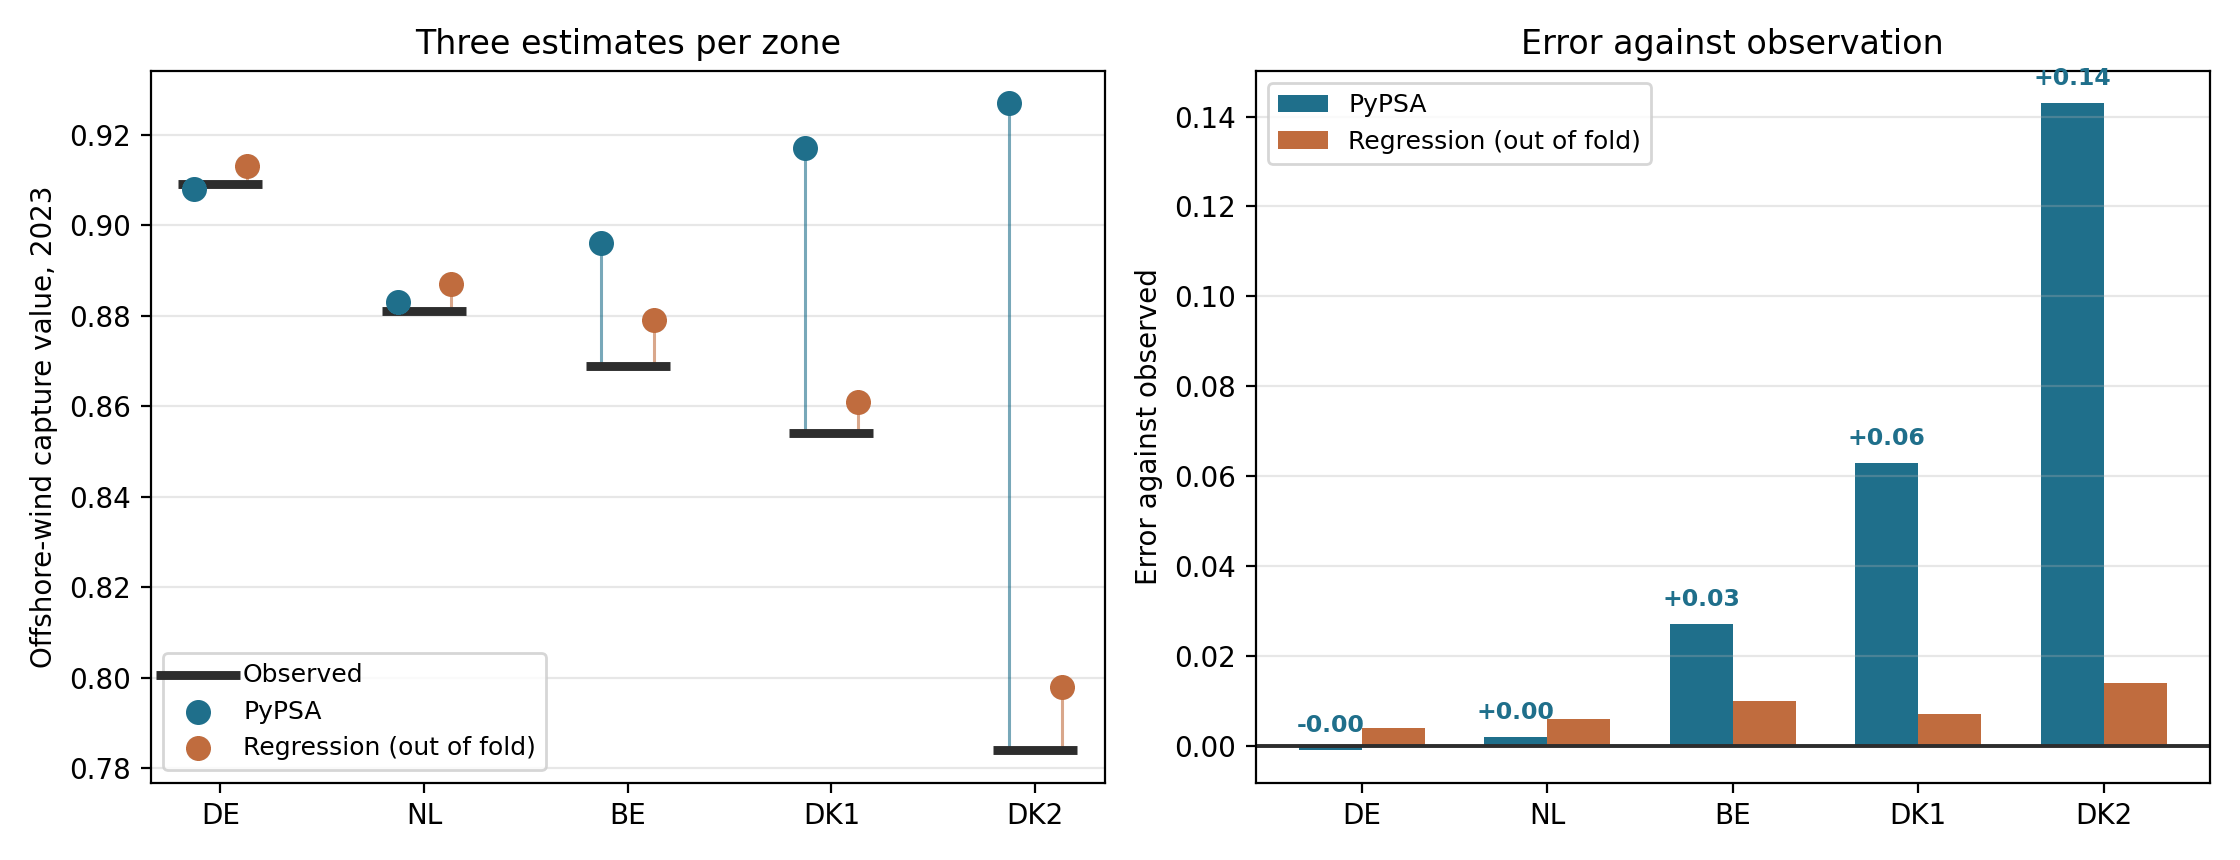
\includegraphics[width=0.95\textwidth]{fig_validation_triangle_2023}
    \caption{The three-way comparison, 2023. Left: the three estimates per zone, observed as the black tick. Right: each model's error. The regression stays within about 0.01 everywhere; the system model's error grows with congestion.}
    \label{fig:triangle}
\end{figure}

\begin{table}[!htb]
\centering\small
\caption{The gap between the two models, decomposed. Channels sum exactly to the
total in every row. Positive means the channel moves the system model's capture
value above the regression model's. Weights are offshore energy.}
\label{tab:gap_channels}
\begin{tabular}{l c c c c c c c}
\toprule
& \textbf{Regression} & \textbf{System} & \textbf{Total} &
\textbf{Constr.} & \textbf{Gener-} & \textbf{Zero} & \textbf{Price} \\
\textbf{Zone} & \textbf{model} & \textbf{model} & \textbf{gap} &
\textbf{residual} & \textbf{ation} & \textbf{floor} & \textbf{shape} \\
\midrule
DE  & 0.913 & 0.888 & $-0.025$ & $-0.014$ & $-0.012$ & $+0.002$ & $+0.002$ \\
NL  & 0.887 & 0.877 & $-0.010$ & $\phantom{-}0.000$ & $+0.009$ & $+0.005$ & $-0.023$ \\
BE  & 0.879 & 0.880 & $+0.001$ & $+0.002$ & $+0.020$ & $+0.002$ & $-0.025$ \\
DK1 & 0.861 & 0.917 & $+0.056$ & $\phantom{-}0.000$ & $+0.007$ & $+0.002$ & $-0.003$ \\
\midrule
Weighted mean & 0.890 & 0.885 & $-0.005$ & $-0.003$ & $+0.004$ & $+0.003$ & $-0.014$ \\
\bottomrule
\end{tabular}
\\[4pt]
{\footnotesize The network-representation channel is $-0.003$ (DE), $-0.001$
(NL), $+0.003$ (BE), $+0.050$ (DK1) and $+0.004$ weighted; it is reported
separately because it is the one channel already corrected in
Section~\ref{sec:division}.}
\end{table}

\begin{figure}[!htb]
    \centering
    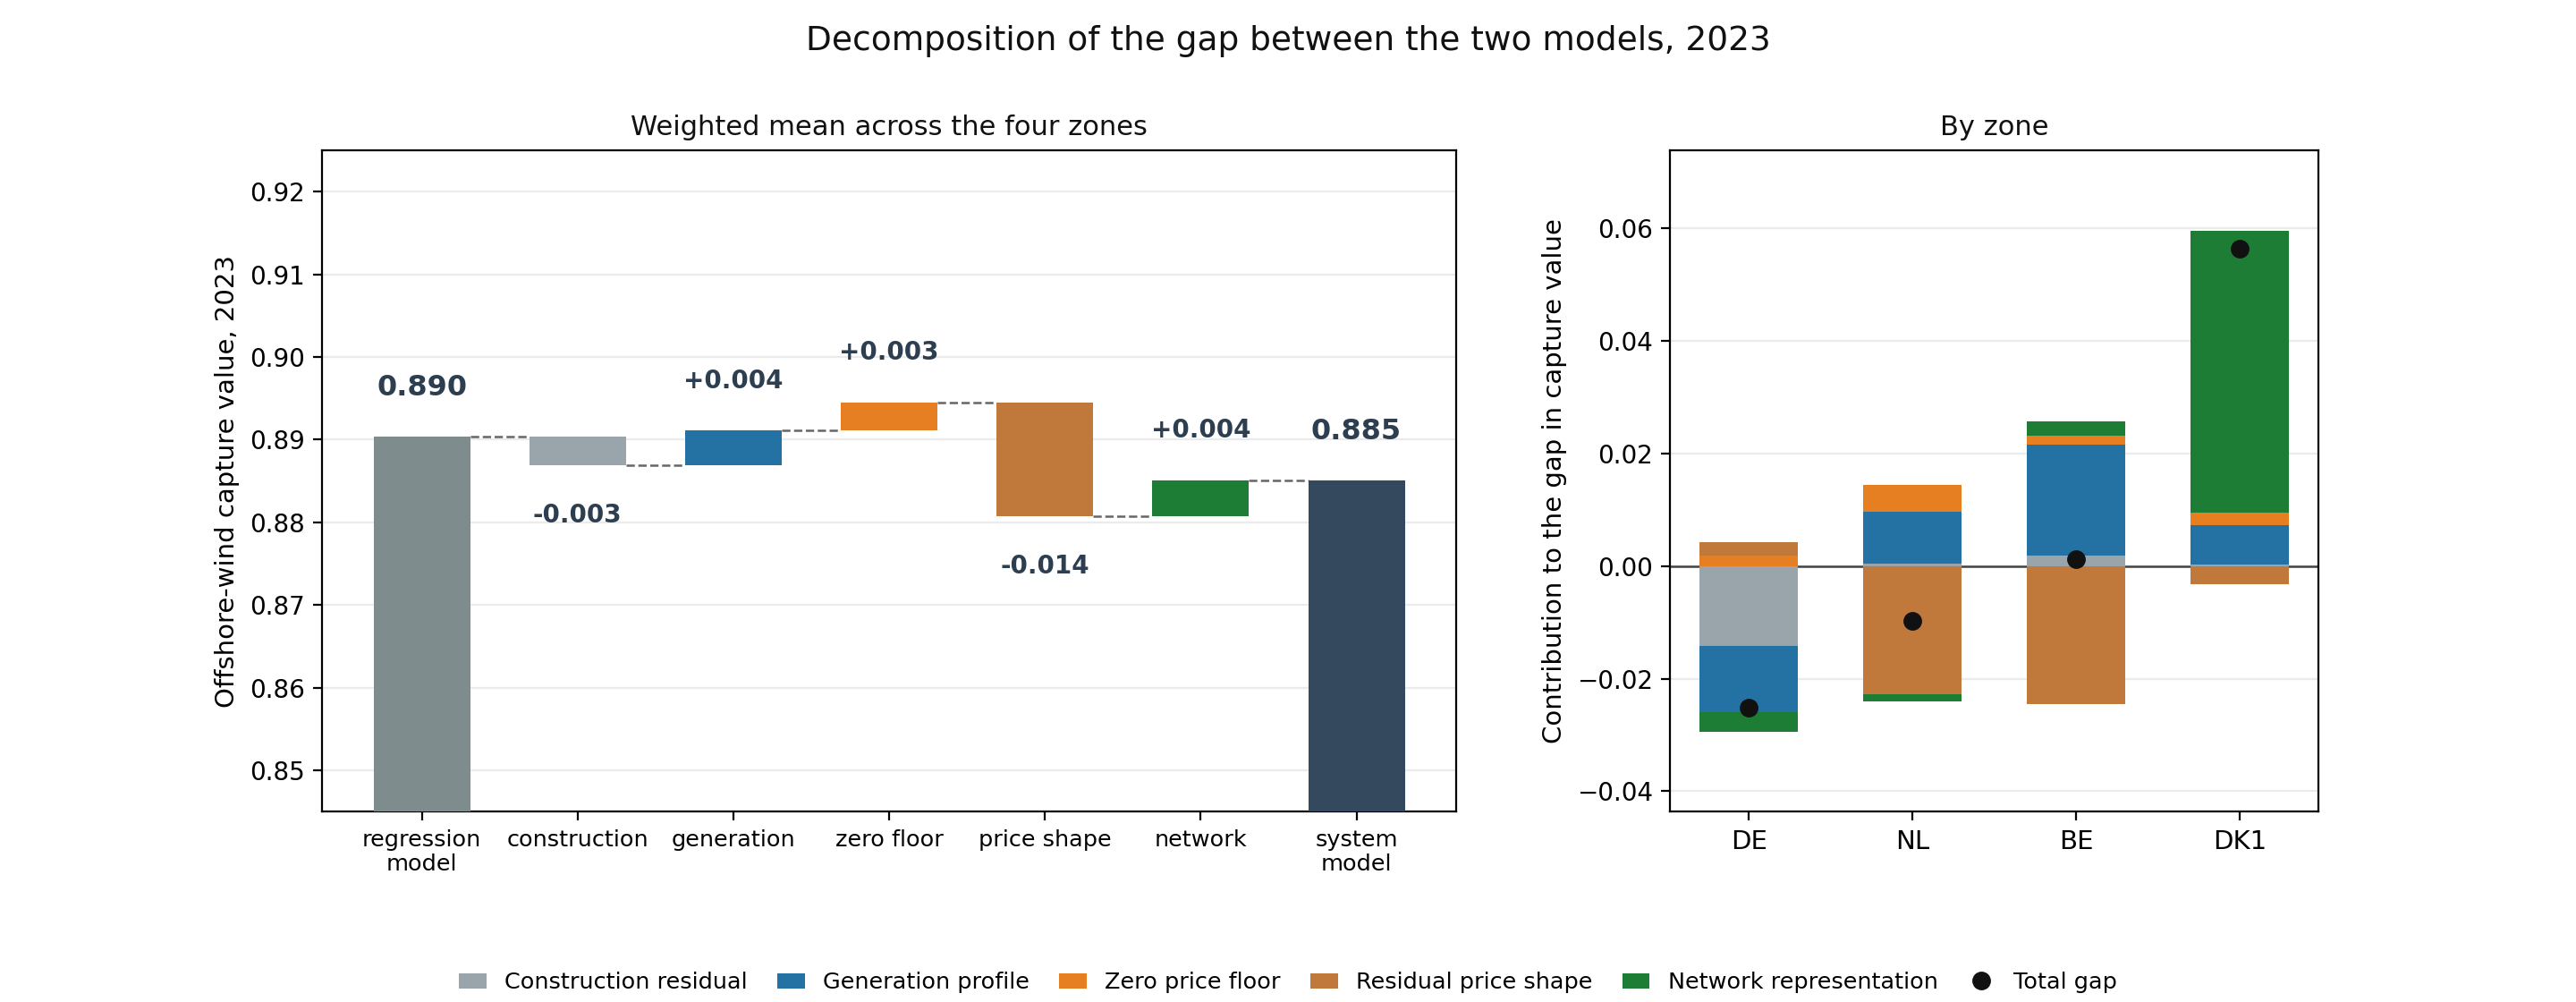
\includegraphics[width=0.98\textwidth]{fig_model_gap_decomposition}
    \caption{Decomposition of the gap between the two models, 2023. Left: the bridge from the regression model's estimate to the system model's, energy-weighted across the four zones. Right: the same channels by zone. Positive values move the system model above the regression model.}
    \label{fig:gap_decomp}
\end{figure}

\begin{figure}[!htb]
    \centering
    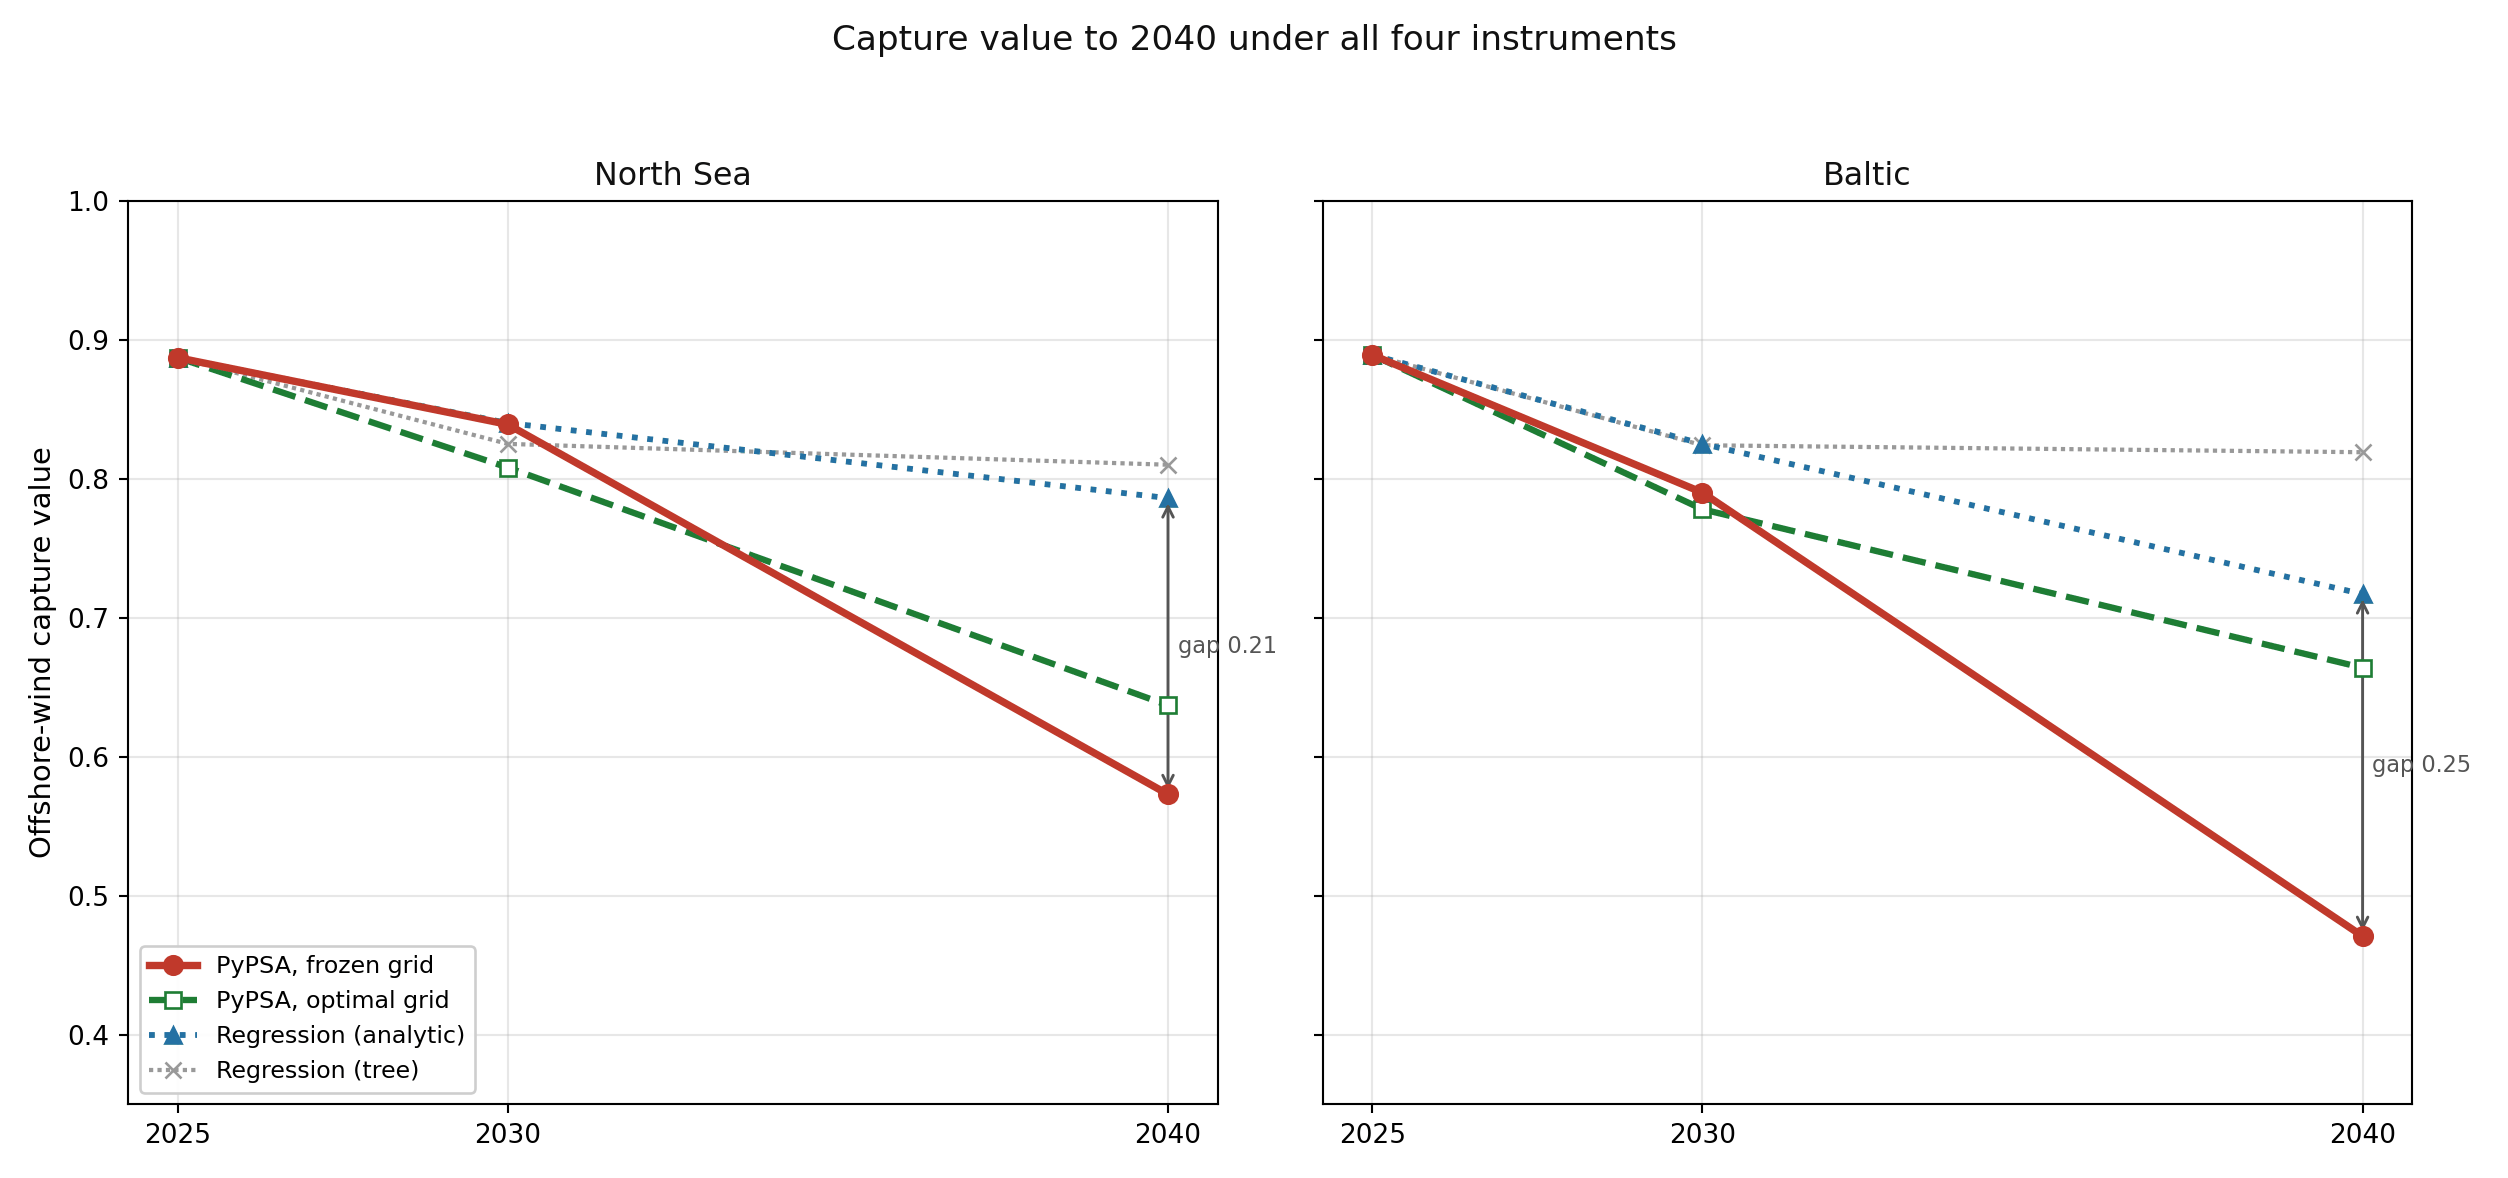
\includegraphics[width=0.88\textwidth]{fig_capture_value_evolution}
    \caption{Every model on one axis, 2025 to 2040. The models
    agree to 2030; at 2040 the regression model returns a constant, the analytical form falls
    gently, and the system model finds the collapse the others cannot.}
    \label{fig:cv_evolution}
\end{figure}

\begin{figure}[!htb]
    \centering
    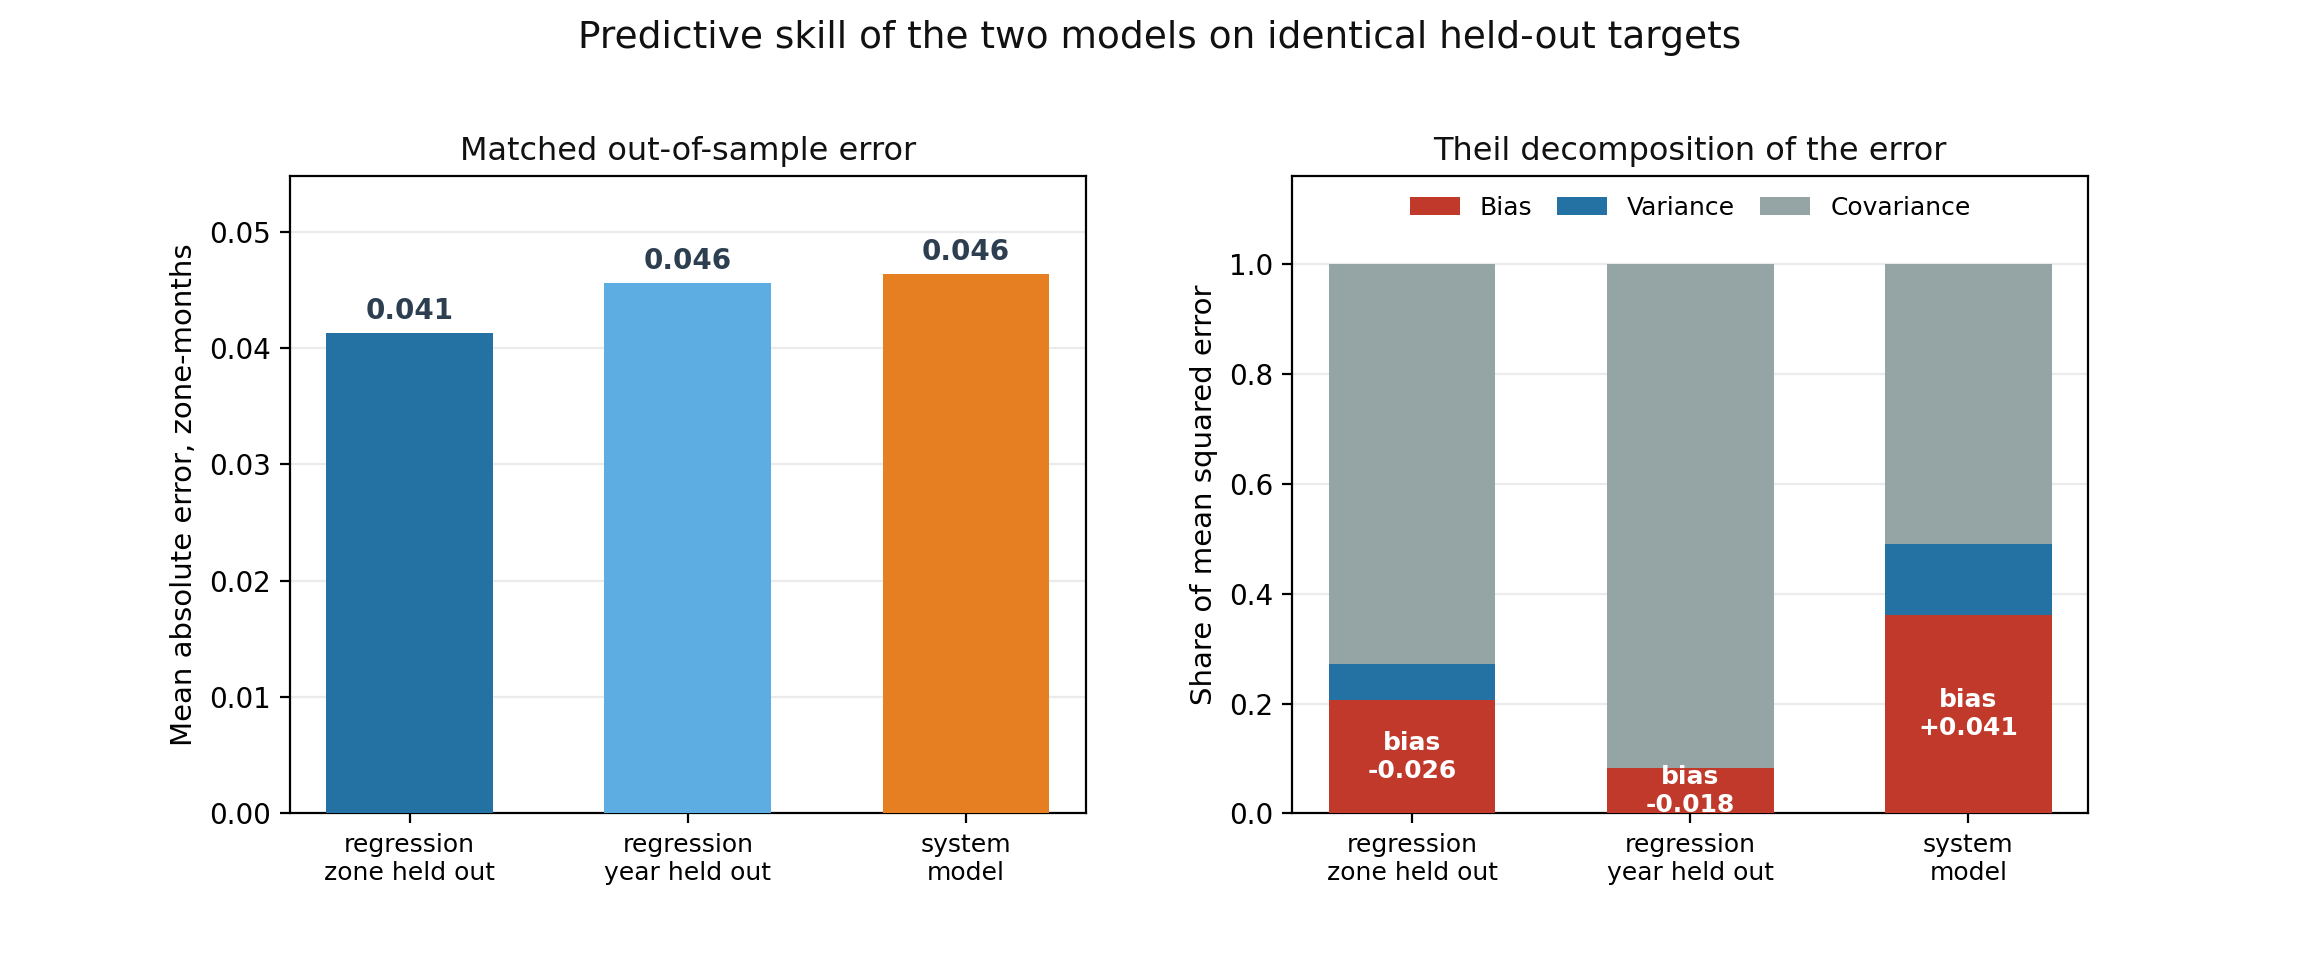
\includegraphics[width=0.92\textwidth]{fig_model_skill}
    \caption{Predictive skill on identical held-out targets. Left: average error,
    indistinguishable across the three schemes. Right: the decomposition of
    squared error into a systematic component, a component from failing to match
    the spread of the observations, and a component from imperfect correlation.
    The system model's error is a third systematic; the regression model's is
    almost entirely imperfect correlation.}
    \label{fig:skill}
\end{figure}

\section{Reproducibility}\label{app:repro}

The entire project is a numbered pipeline: scripts 1.01 to 1.20 (system model), 2.01 to 2.13 (regression model), and 3.01 (the comparison with observation), each reading its predecessors' outputs from disk and writing
its own next to them. A single refresh chain re-solves everything from the
prepared networks to the final tables in about three hours on a workstation
(Apple Silicon, Gurobi academic licence); individual scenario solves take
about 90 seconds at solver parity. Every headline number regenerates from
public data: ENTSO-E Transparency, ERA5 via Open-Meteo and atlite, TYNDP
2024 workbooks, and open cost data. Configuration files pin every assumption
of Appendix~\ref{app:assumptions}; staleness guards (input modification
times recorded next to fitted outputs) make outdated results detectable. A
line-by-line audit log of the one major repair cycle, with before and after
values, is kept in the project repository.

\begin{table}[!htb]
\centering
\small
\caption{Inventory of system-model runs. All solves use the identical model version, solver configuration, and
corrections of this chapter; only the
stated dimension varies.}
\label{tab:runs}
\begin{tabular}{l c p{7.2cm}}
\toprule
\textbf{Run set} & \textbf{Solves} & \textbf{Purpose} \\
\midrule
Historical baselines & 3 & 2019, 2023, and 2024 calibration years \\
Canonical scenarios & 6 & 2030/2040, central and high Baltic buildouts, two
2040 demand pathways \\
Gas-price grid & 15 & three buildouts $\times$ five gas prices, 15 to
120~\euro/MWh \\
Grid bracket & 6 & the six scenarios with optimisable transmission \\
Surrogate training & 55 & 50 Latin-hypercube points plus 5 scenario anchors,
three-hourly, harvested alongside the 21 full-hourly solves above \\
Resolution check & 2 & two design points re-solved at full resolution \\
\bottomrule
\end{tabular}
\end{table}
Table~\ref{tab:versions} pins the software environment behind every solve
and fit.

\begin{table}[!htb]
\centering\small
\caption{The software environment. All versions are those used for the
reported runs; the regression stack is pinned because untuned library defaults
are version-dependent.}
\label{tab:versions}
\begin{tabular}{l l l l}
\toprule
Python & 3.13 & PyPSA-Eur & v2026.02.0 (commit 23c2fac7) \\
pypsa & 1.2.0 & snakemake & 9.20.0 \\
Gurobi & 13.0.2 (academic) & atlite & 0.6.1 \\
xgboost & 3.2.0 & scikit-learn & 1.8.0 \\
pandas & 2.3.3 & numpy & 2.4.3 \\
\bottomrule
\end{tabular}
\end{table}

% ============================================================================
\section{Spatial Atlas}\label{app:atlas}
% ============================================================================

The main text carries one map per argument. This appendix carries the full
spatial series behind them, so that every field is available at all three
horizons rather than only at the year the argument needed. Each family is built
on the same footing: the high-resolution capacity-factor field of
Section~\ref{sec:cost_field}, water depth and distance from GEBCO, and per-zone
capture values read from the solved networks of Section~\ref{sec:projection}. All
maps share a fixed colour scale within their family so that the three horizons
are directly comparable; a field that changes colour between 2025 and 2040 has changed in value.

\FloatBarrier
\subsection*{F.1 The resource field}

\begin{figure}[!htb]
    \centering
    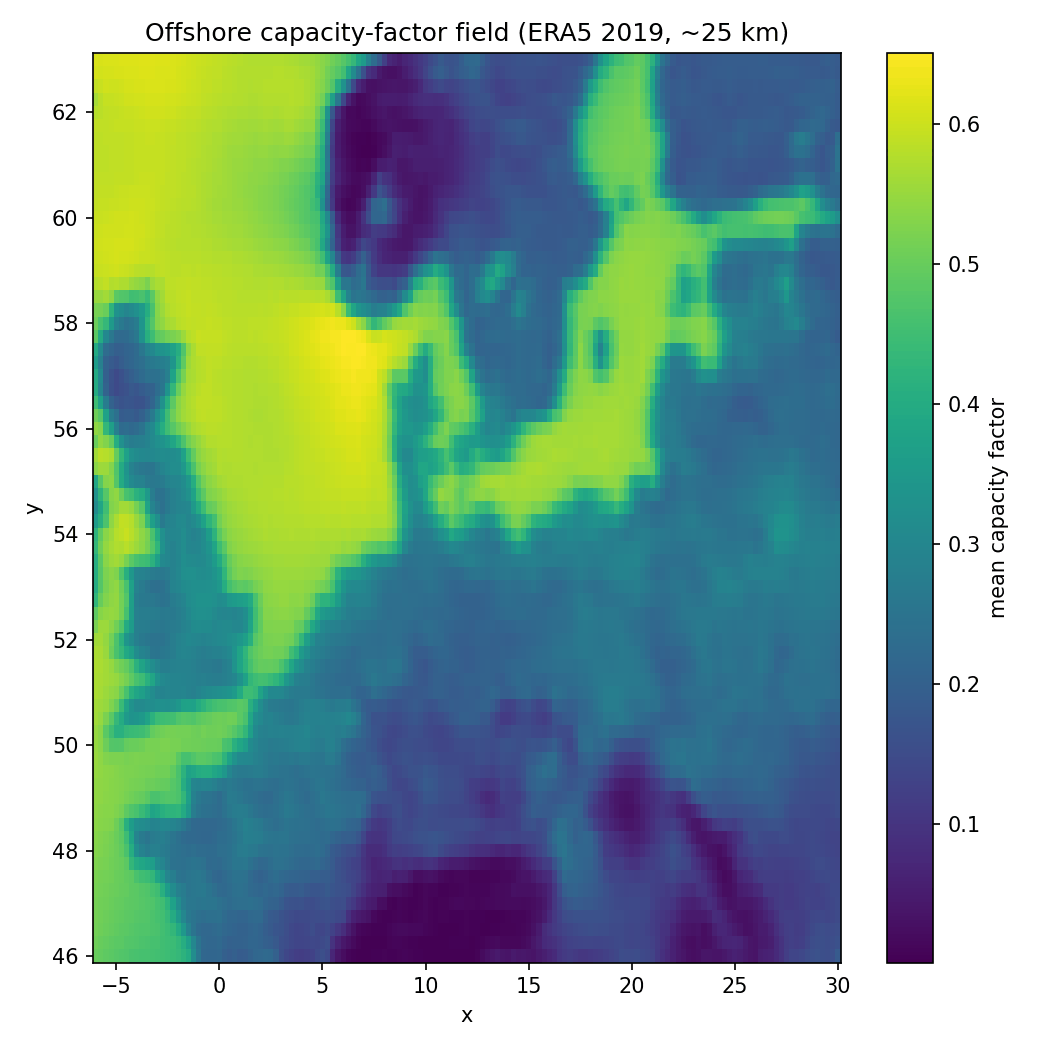
\includegraphics[width=0.80\textwidth]{fig_cf_field_preview}
    \caption{The offshore capacity-factor field across both shelves, built once
    from the Global Wind Atlas at roughly 2~km resolution and used as the common
    resource layer for every economic map that follows. The gradient from the
    open North Sea to the eastern Baltic is the physical starting point for the
    whole comparison, and it is year-independent: the wind field is identical in every year, so the changes in the maps that
    follow come from value and cost.}
    \label{fig:cf_field}
\end{figure}

\FloatBarrier
\subsection*{F.2 Capture value under an optimal grid}

Figures~\ref{fig:heatmap_2025} to~\ref{fig:heatmap_2040} in the main text show
capture value on the frozen grid. The counterfactual matters as much, since the
difference between the two is the congestion component isolated in
Section~\ref{sec:decomposition}. The maps below repeat the sequence with
transmission expanded to the cost optimum.

\begin{figure}[!htb]
    \centering
    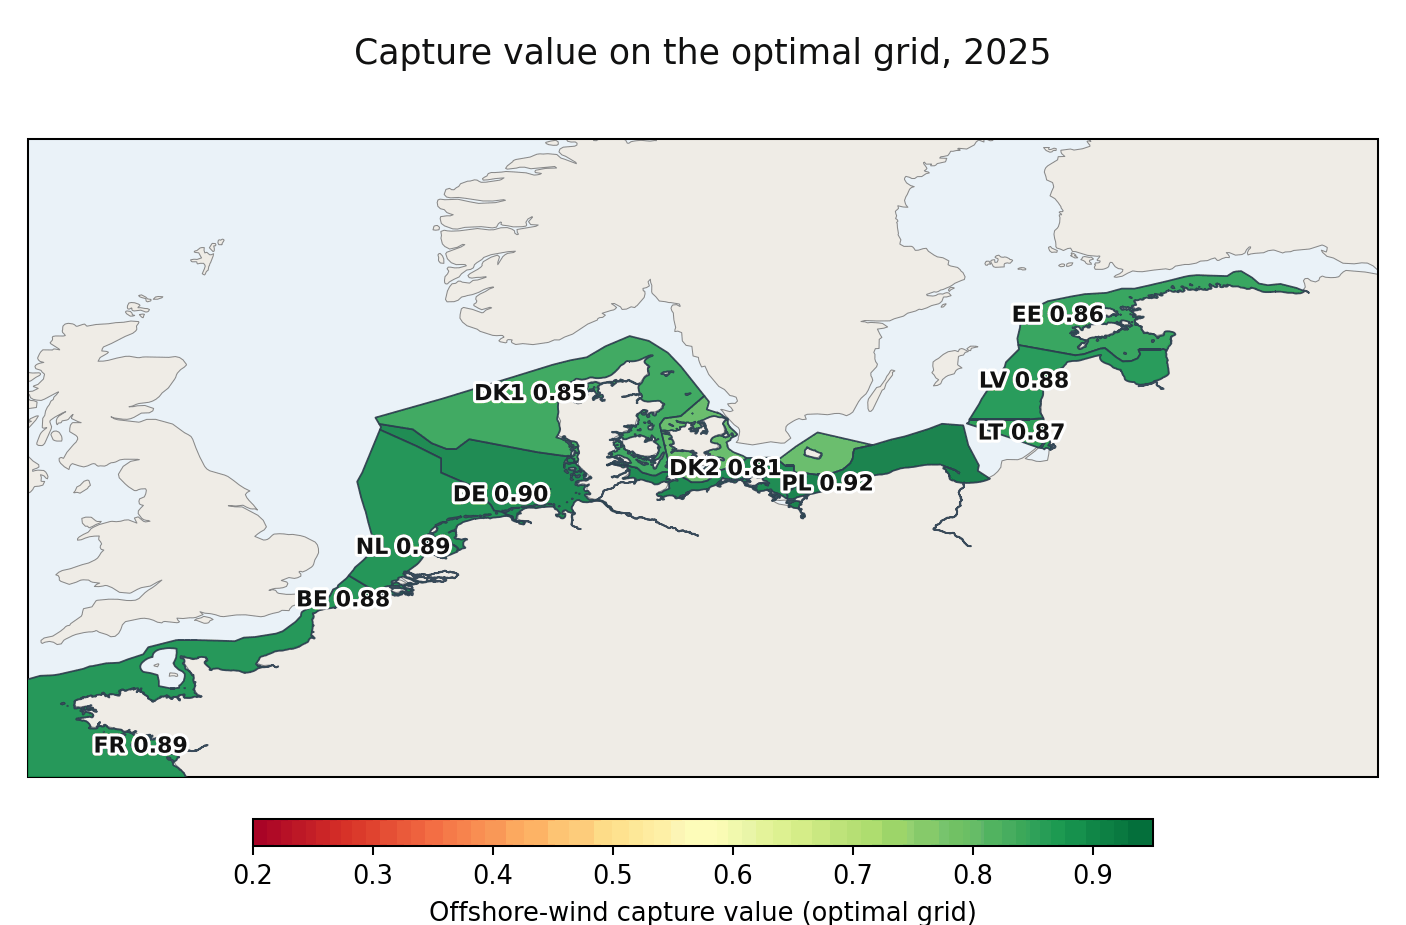
\includegraphics[width=0.72\textwidth]{fig_heatmap_opt_2025}
    \caption{Capture value on the cost-optimal grid, 2025. At today's
    penetration the grid assumption barely matters and the field is
    indistinguishable from the frozen case.}
    \label{fig:heatmap_opt_2025}
\end{figure}

\begin{figure}[!htb]
    \centering
    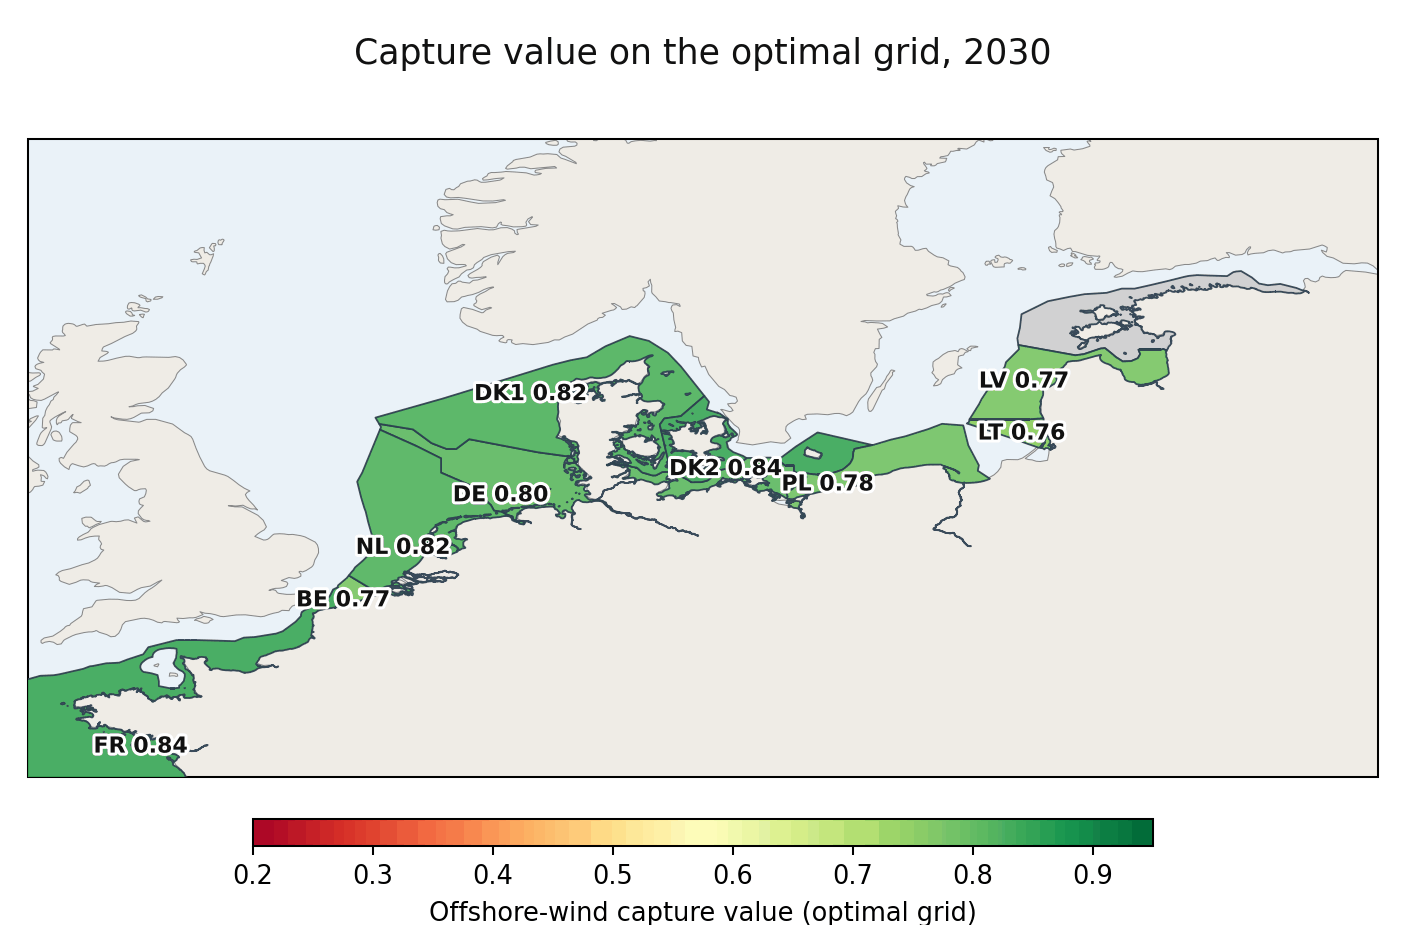
\includegraphics[width=0.72\textwidth]{fig_heatmap_opt_2030}
    \caption{Capture value on the cost-optimal grid, 2030. The bracket is still
    almost nil: congestion has not yet begun to bind.}
    \label{fig:heatmap_opt_2030}
\end{figure}

\begin{figure}[!htb]
    \centering
    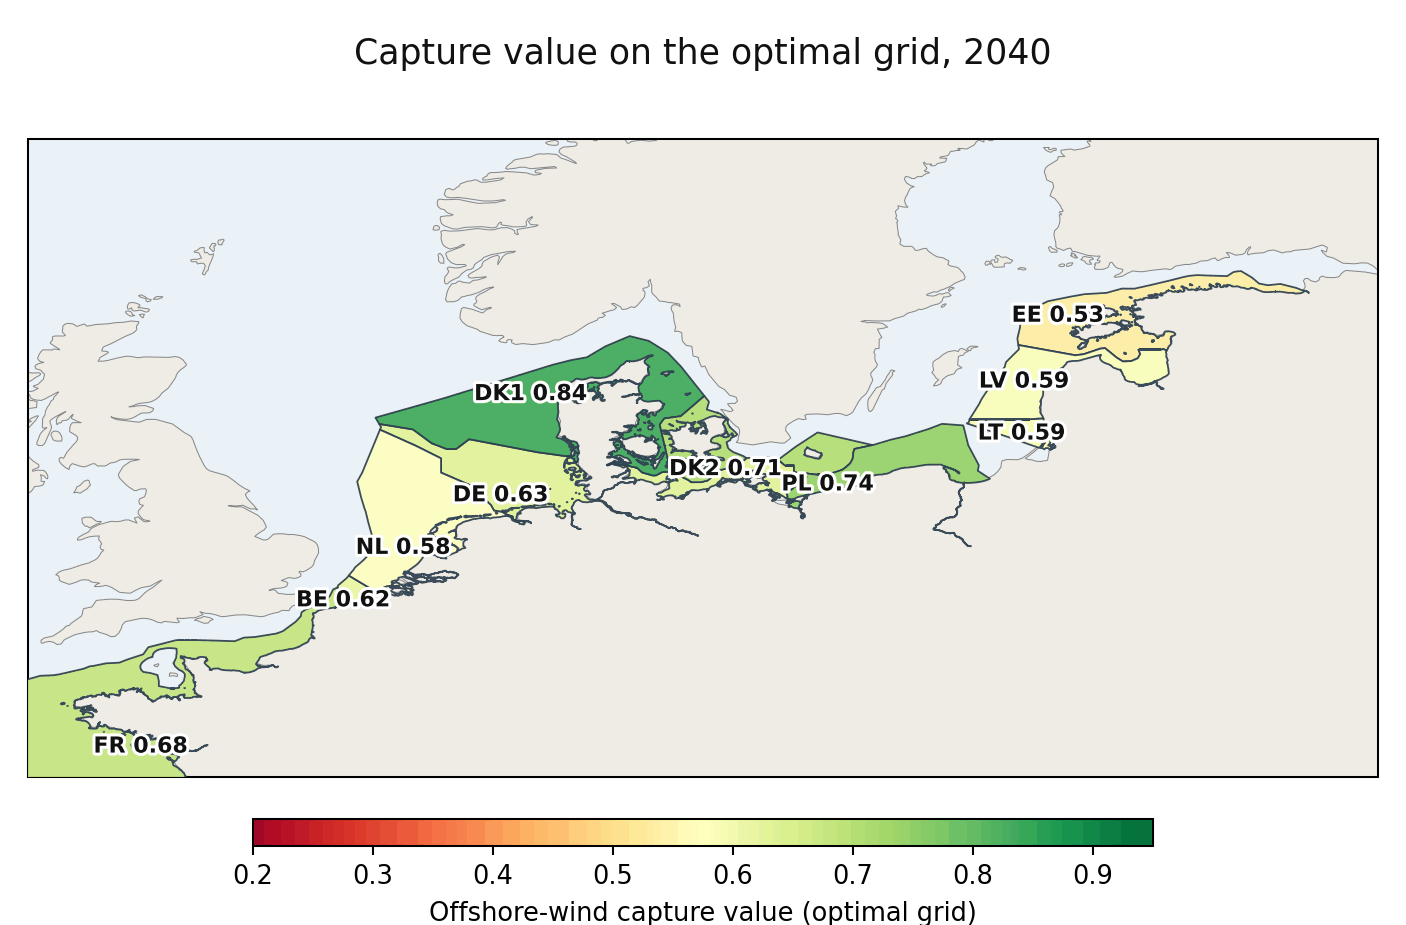
\includegraphics[width=0.72\textwidth]{fig_heatmap_opt_2040}
    \caption{Capture value on the cost-optimal grid, 2040. Compared with
    Figure~\ref{fig:heatmap_2040} the eastern Baltic recovers most, which is the
    spatial expression of the reversal: the zones that lose the most to a frozen
    network are the ones an expanded network restores.}
    \label{fig:heatmap_opt_2040}
\end{figure}

\FloatBarrier
\subsection*{F.3 Levelised cost across the shelf}

The cost field is the standard output of the spatial assessment literature
\cite{Bosch2019} and the baseline against which the value-adjusted metric is
compared. It falls with technology learning and is otherwise governed by depth,
distance and resource.

\begin{figure}[!htb]
    \centering
    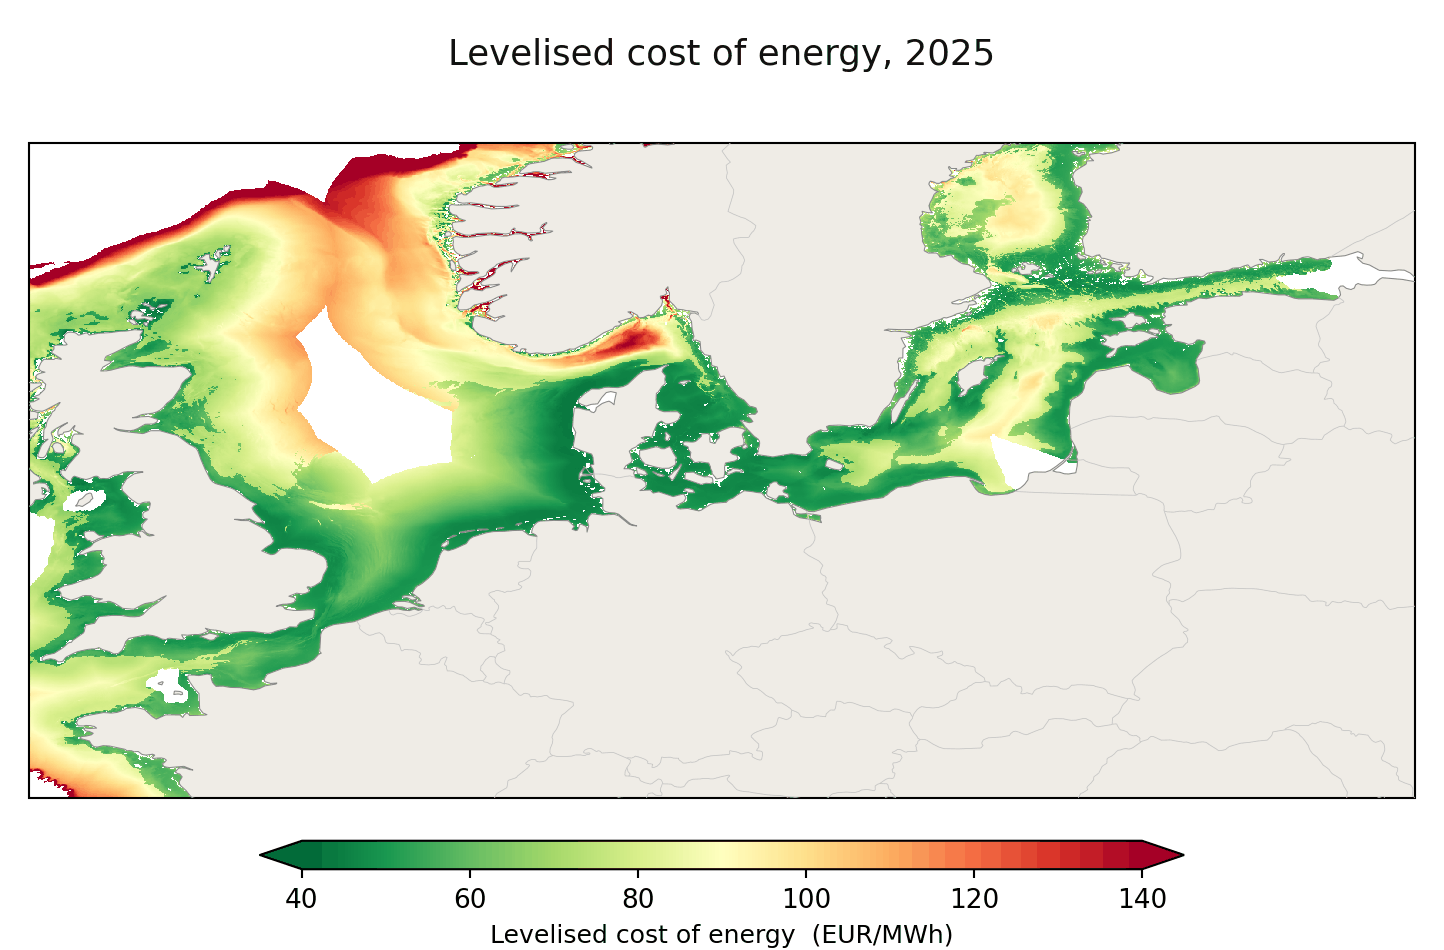
\includegraphics[width=0.72\textwidth]{fig_cost_lcoe_2025}
    \caption{Levelised cost of energy by location, 2025. Cheap sites cluster in
    the shallow southern North Sea and the western Baltic; the deep Norwegian
    trench never clears the floating-foundation premium.}
    \label{fig:cost_2025}
\end{figure}

\begin{figure}[!htb]
    \centering
    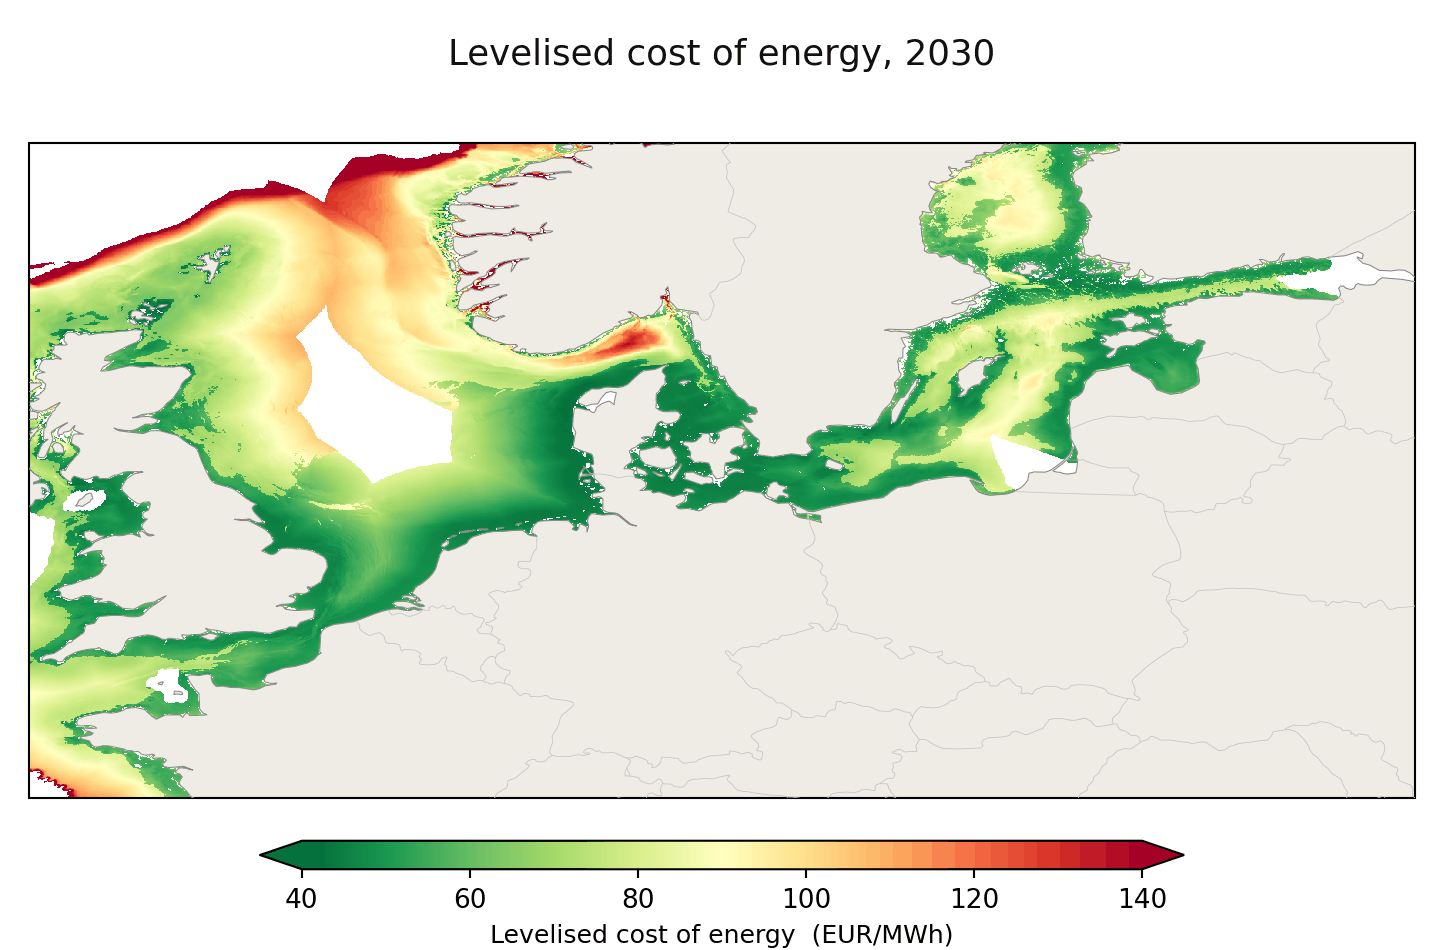
\includegraphics[width=0.72\textwidth]{fig_cost_lcoe_2030}
    \caption{Levelised cost by location, 2030. The whole field dims as capital
    costs fall; the spatial pattern is unchanged.}
    \label{fig:cost_2030}
\end{figure}

\begin{figure}[!htb]
    \centering
    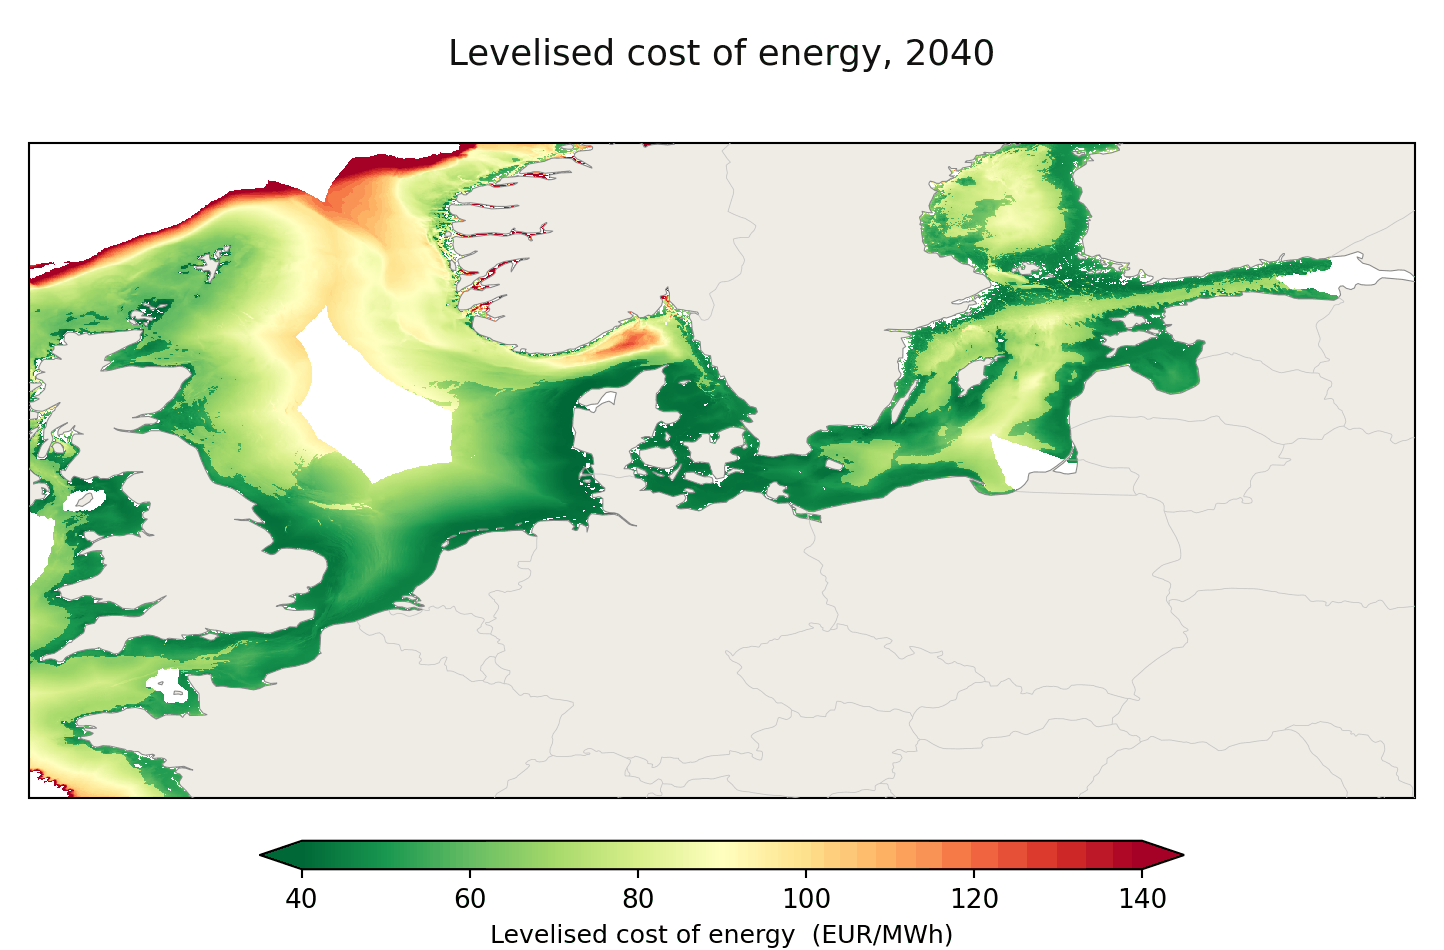
\includegraphics[width=0.72\textwidth]{fig_cost_lcoe_2040}
    \caption{Levelised cost by location, 2040. On cost alone the shelf looks
    steadily more attractive over time, which is precisely the impression the
    value-adjusted maps of Section~F.4 overturn.}
    \label{fig:cost_2040}
\end{figure}

\FloatBarrier
\subsection*{F.4 Value-adjusted cost}

Dividing the cost field by capture value gives the wholesale price a site must
earn to break even (Equation~\ref{eq:vlcoe}). The 2040 map appears in the main
text as Figure~\ref{fig:vlcoe}; the earlier horizons complete the series
and show the direction of travel.

\begin{figure}[!htb]
    \centering
    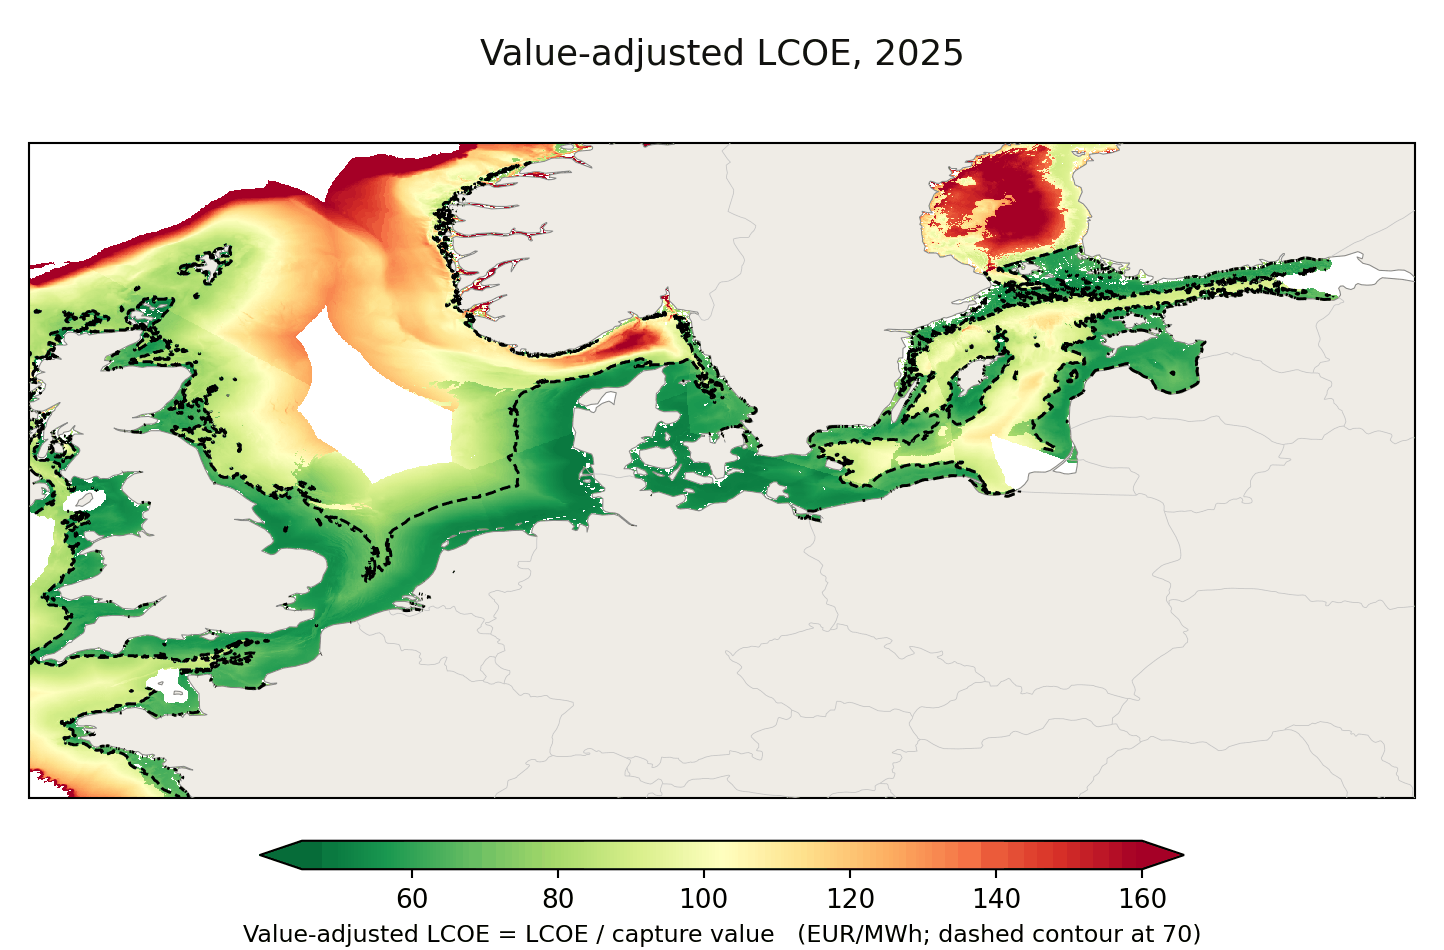
\includegraphics[width=0.72\textwidth]{fig_vlcoe_2025}
    \caption{Value-adjusted cost of energy, 2025. With capture values near 0.9
    across both shelves the field sits close to the raw cost map.}
    \label{fig:vlcoe_2025}
\end{figure}

\begin{figure}[!htb]
    \centering
    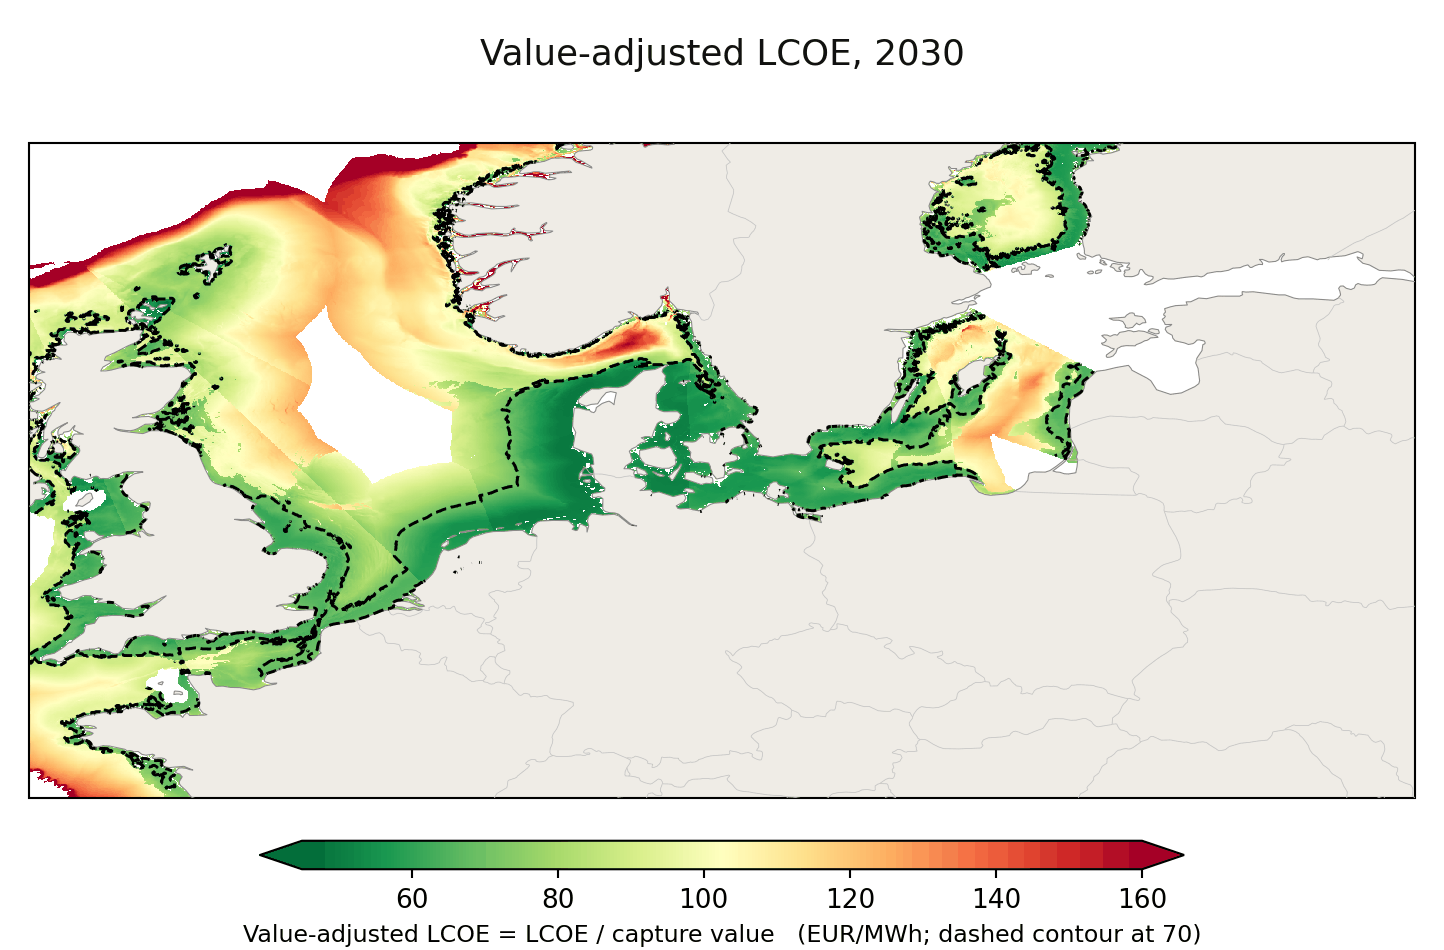
\includegraphics[width=0.72\textwidth]{fig_vlcoe_2030}
    \caption{Value-adjusted cost, 2030. The eastern Baltic begins to separate
    from its cost map as its capture value falls faster than its cost.}
    \label{fig:vlcoe_2030}
\end{figure}

Read against Figures~\ref{fig:cost_2025} to~\ref{fig:cost_2040}, the pair of
series states the thesis result in its most compact form. The cost field
improves monotonically with learning while the value-adjusted field deteriorates,
and the divergence between them is cannibalisation expressed in euros per
megawatt-hour rather than as a ratio.

\FloatBarrier
\subsection*{F.5 Net value}

Net value subtracts annualised cost from revenue and answers whether a site pays
at all, rather than what price it needs. The series opens with the 2040 map
(Figure~\ref{fig:netvalue}), the horizon the body's argument turns on; the
earlier horizons follow.

\begin{figure}[!htb]
    \centering
    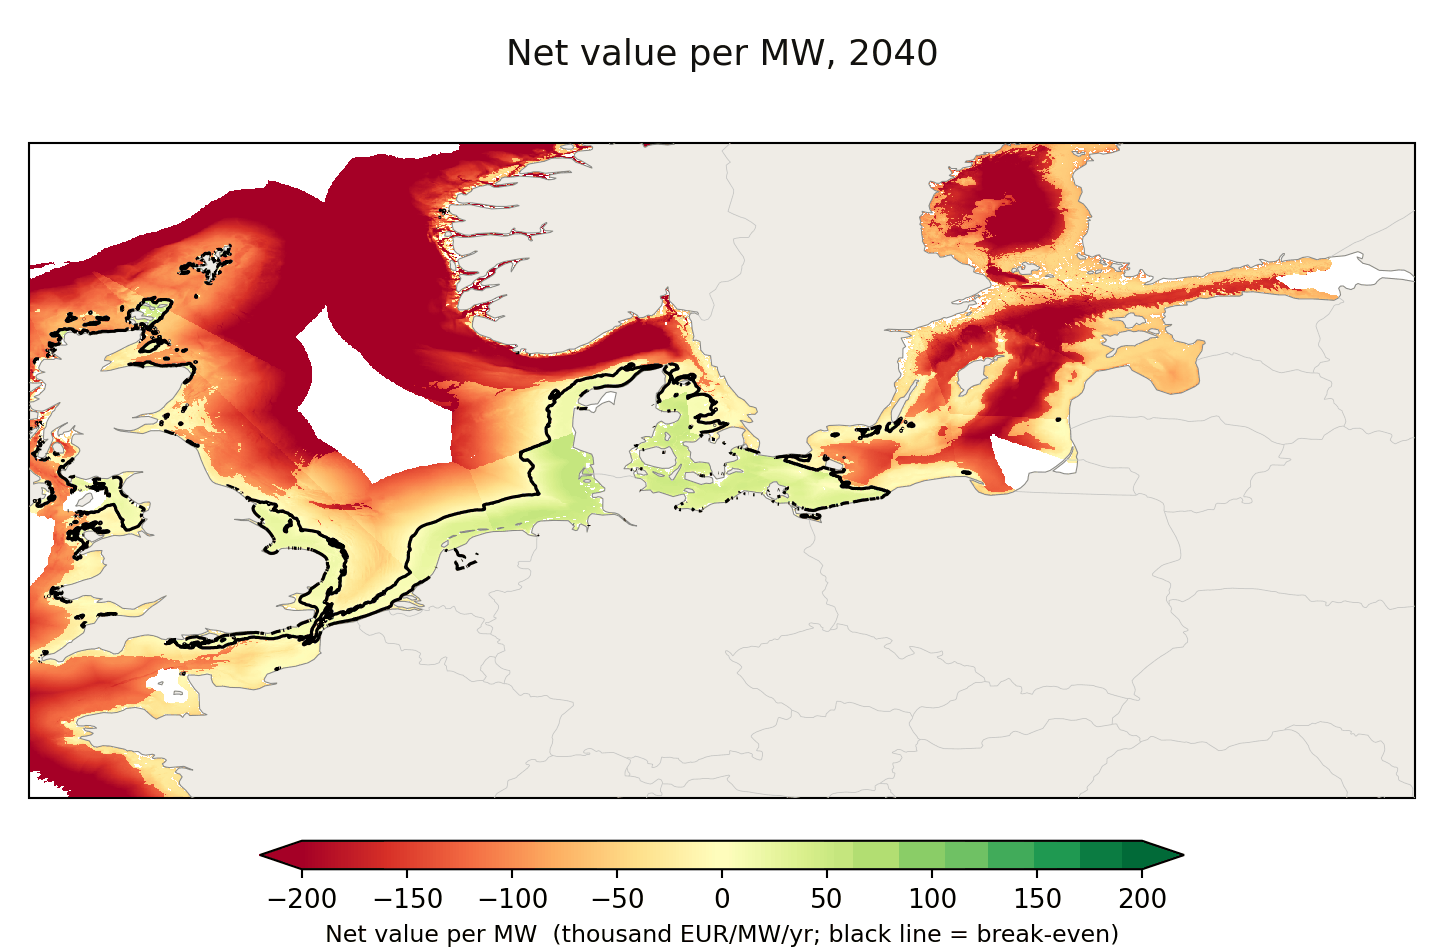
\includegraphics[width=0.6\textwidth]{fig_netvalue_2040}
    \caption{Merchant net value per megawatt in 2040, captured revenue less
    annualised cost. Green is profitable at merchant prices; the profitable shelf
    shrinks from about 48\% of buildable area in 2025 to 12\% by 2040, as value is withdrawn while cost continues to fall.}
    \label{fig:netvalue}
\end{figure}

\begin{figure}[!htb]
    \centering
    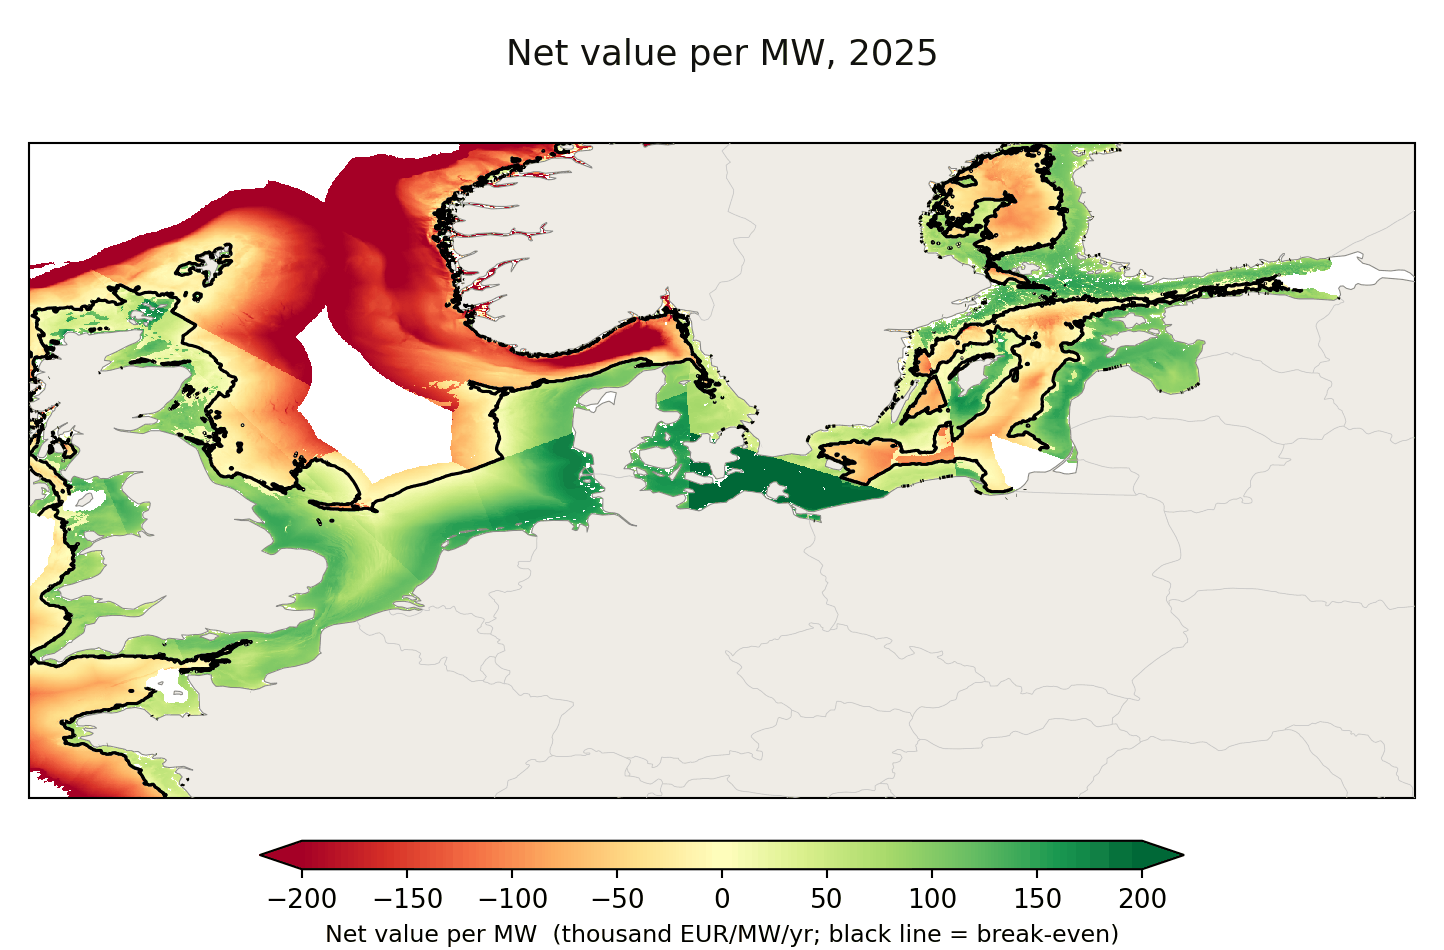
\includegraphics[width=0.72\textwidth]{fig_netvalue_2025}
    \caption{Net value per megawatt, 2025. Roughly half the buildable shelf is
    merchant-profitable at today's capture values and prices.}
    \label{fig:netvalue_2025}
\end{figure}

\begin{figure}[!htb]
    \centering
    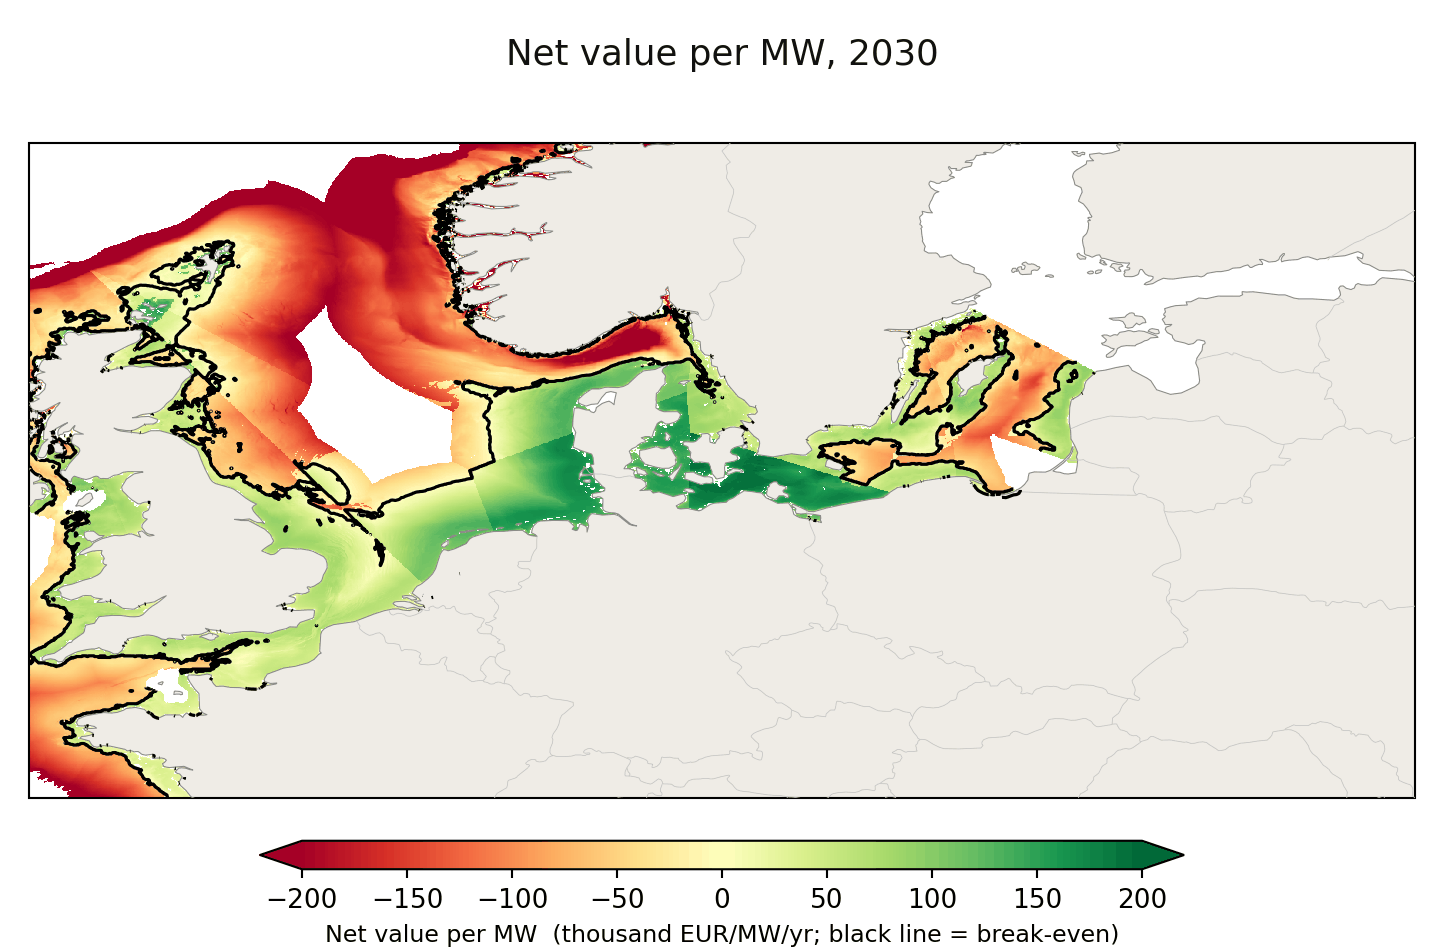
\includegraphics[width=0.72\textwidth]{fig_netvalue_2030}
    \caption{Net value per megawatt, 2030. The profitable area has begun to
    contract toward the shallow, high-resource core.}
    \label{fig:netvalue_2030}
\end{figure}

\FloatBarrier
\subsection*{F.6 Revenue density}

The revenue-density series superimposes the resource field on the per-zone
capture value and price, giving revenue per unit area rather than per megawatt.
It is the most granular of the spatial products, built on the roughly 2~km Global
Wind Atlas field.

\begin{figure}[!htb]
    \centering
    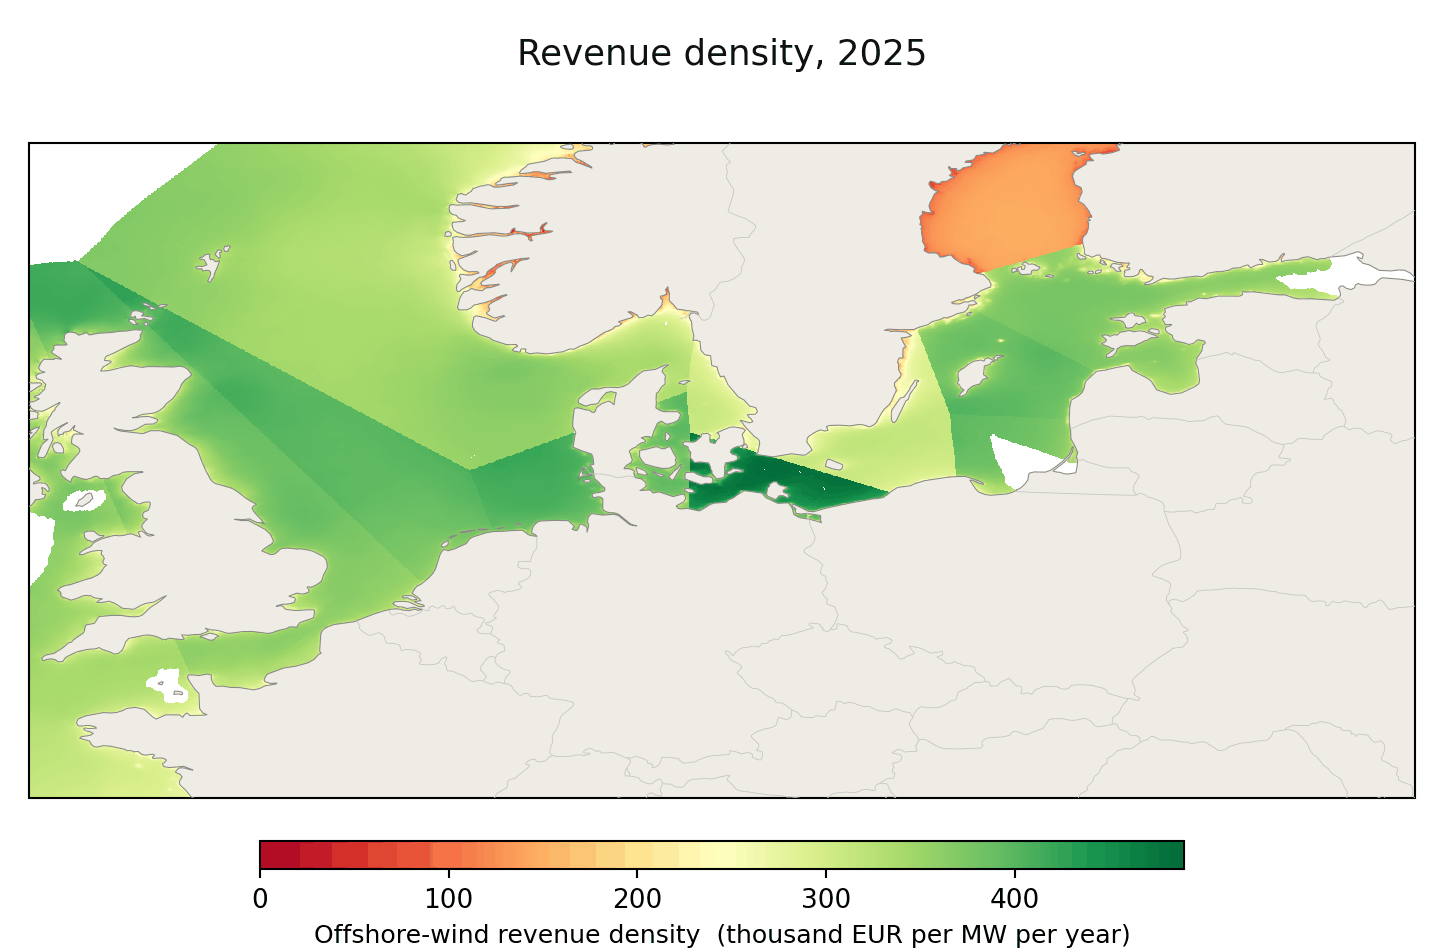
\includegraphics[width=0.72\textwidth]{fig_revenue_density_hires_2025}
    \caption{Revenue density across both shelves, 2025.}
    \label{fig:revdens_2025}
\end{figure}

\begin{figure}[!htb]
    \centering
    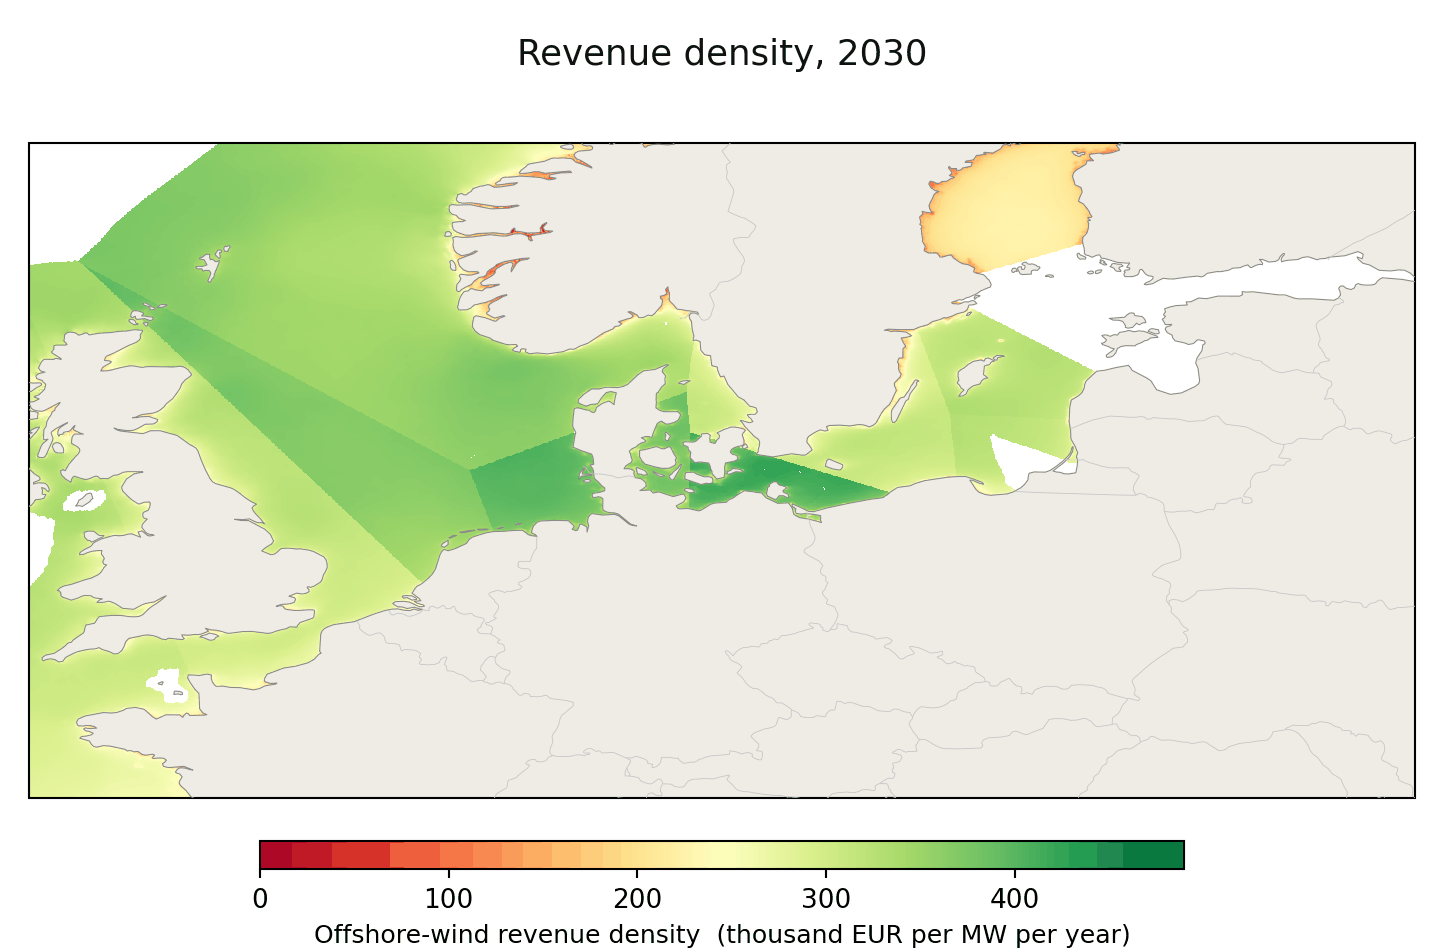
\includegraphics[width=0.72\textwidth]{fig_revenue_density_hires_2030}
    \caption{Revenue density, 2030.}
    \label{fig:revdens_2030}
\end{figure}

\begin{figure}[!htb]
    \centering
    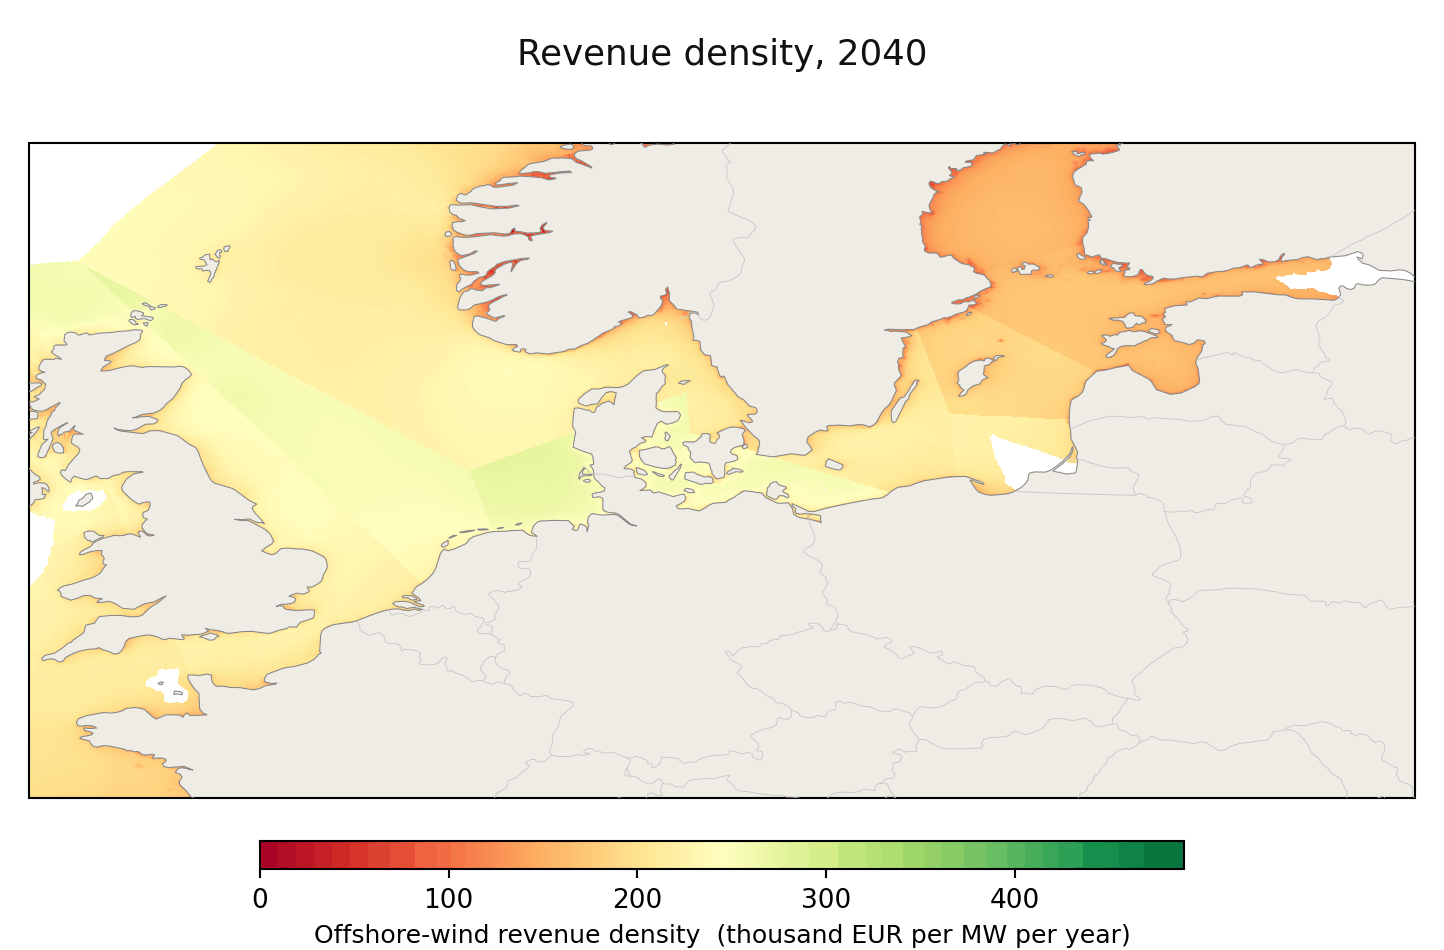
\includegraphics[width=0.72\textwidth]{fig_revenue_density_hires_2040}
    \caption{Revenue density, 2040. The contraction toward the German Bight and
    the shallow western Baltic is the same pattern the site ranking of
    Section~\ref{sec:site_ranking} produces numerically.}
    \label{fig:revdens_2040}
\end{figure}

\FloatBarrier
\subsection*{F.7 Candidate areas on the value grid}

\begin{figure}[!htb]
    \centering
    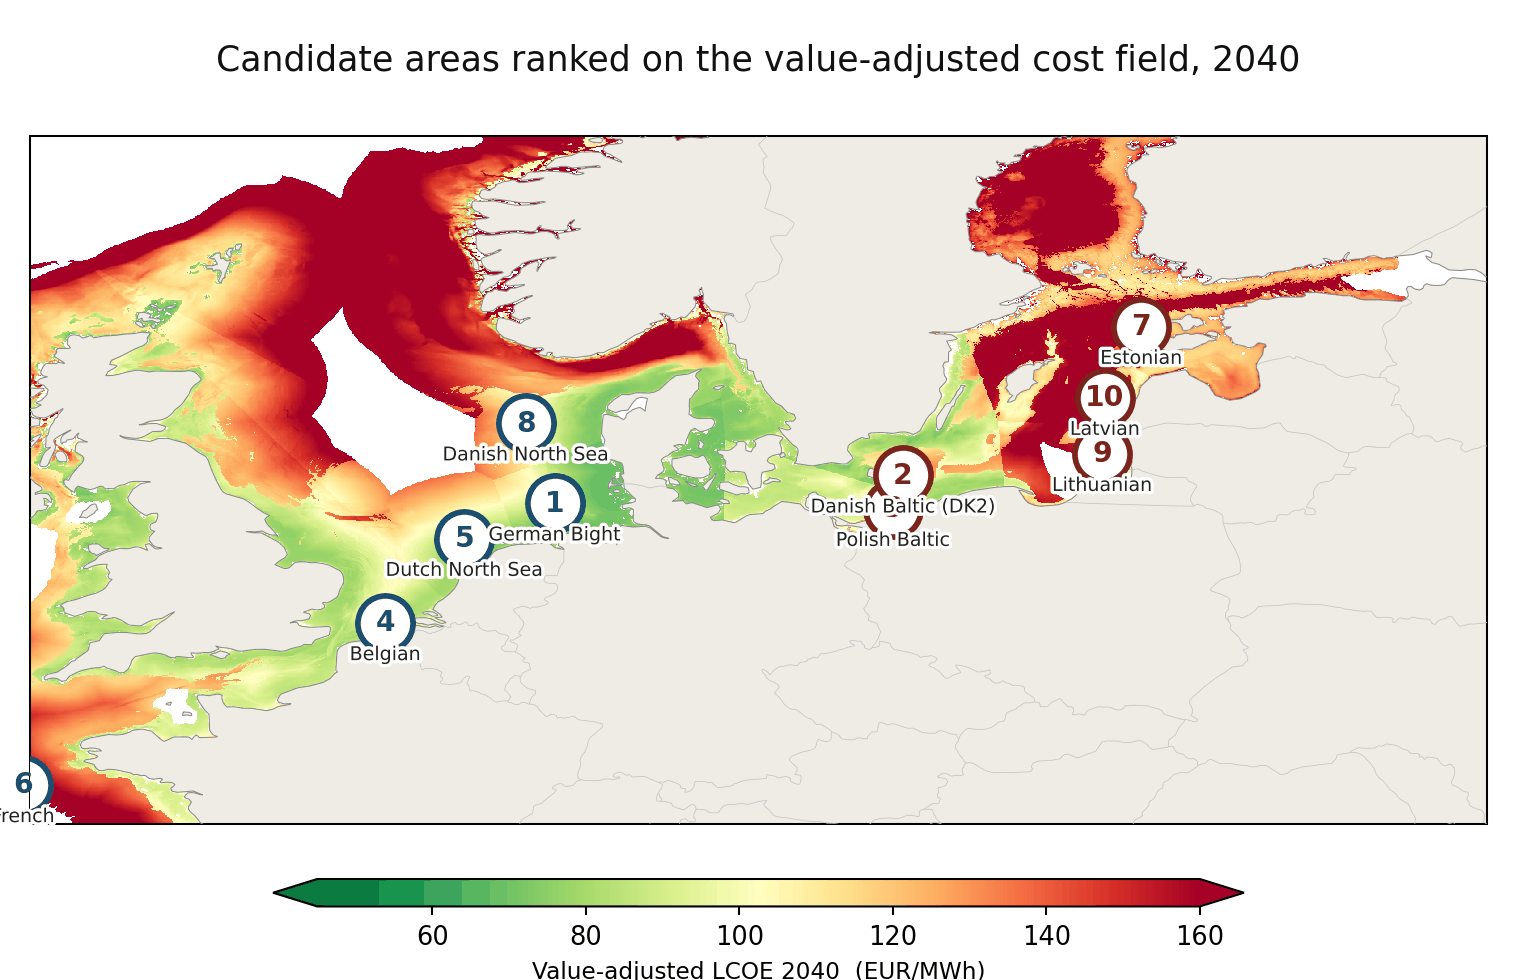
\includegraphics[width=0.86\textwidth]{fig_site_ranking_map}
    \caption{The ten candidate development areas positioned on the 2040
    value-adjusted field, which is the spatial backing for the ranking reported
    in Section~\ref{sec:site_ranking}. Circled numbers give the value-adjusted
    rank, 1 the best; blue marks North Sea areas, red Baltic. The areas that
    fall in the ranking are visibly those sitting in the reddest water.}
    \label{fig:site_ranking_map}
\end{figure}

% ============================================================================
\FloatBarrier
\section{Supplementary Figures}\label{app:supplementary}
% ============================================================================

This appendix holds diagnostics and intermediate results referenced in passing by
the main text, grouped by the chapter they support.

\FloatBarrier
\subsection*{G.1 Model resolution}



\begin{figure}[!htb]
    \centering
    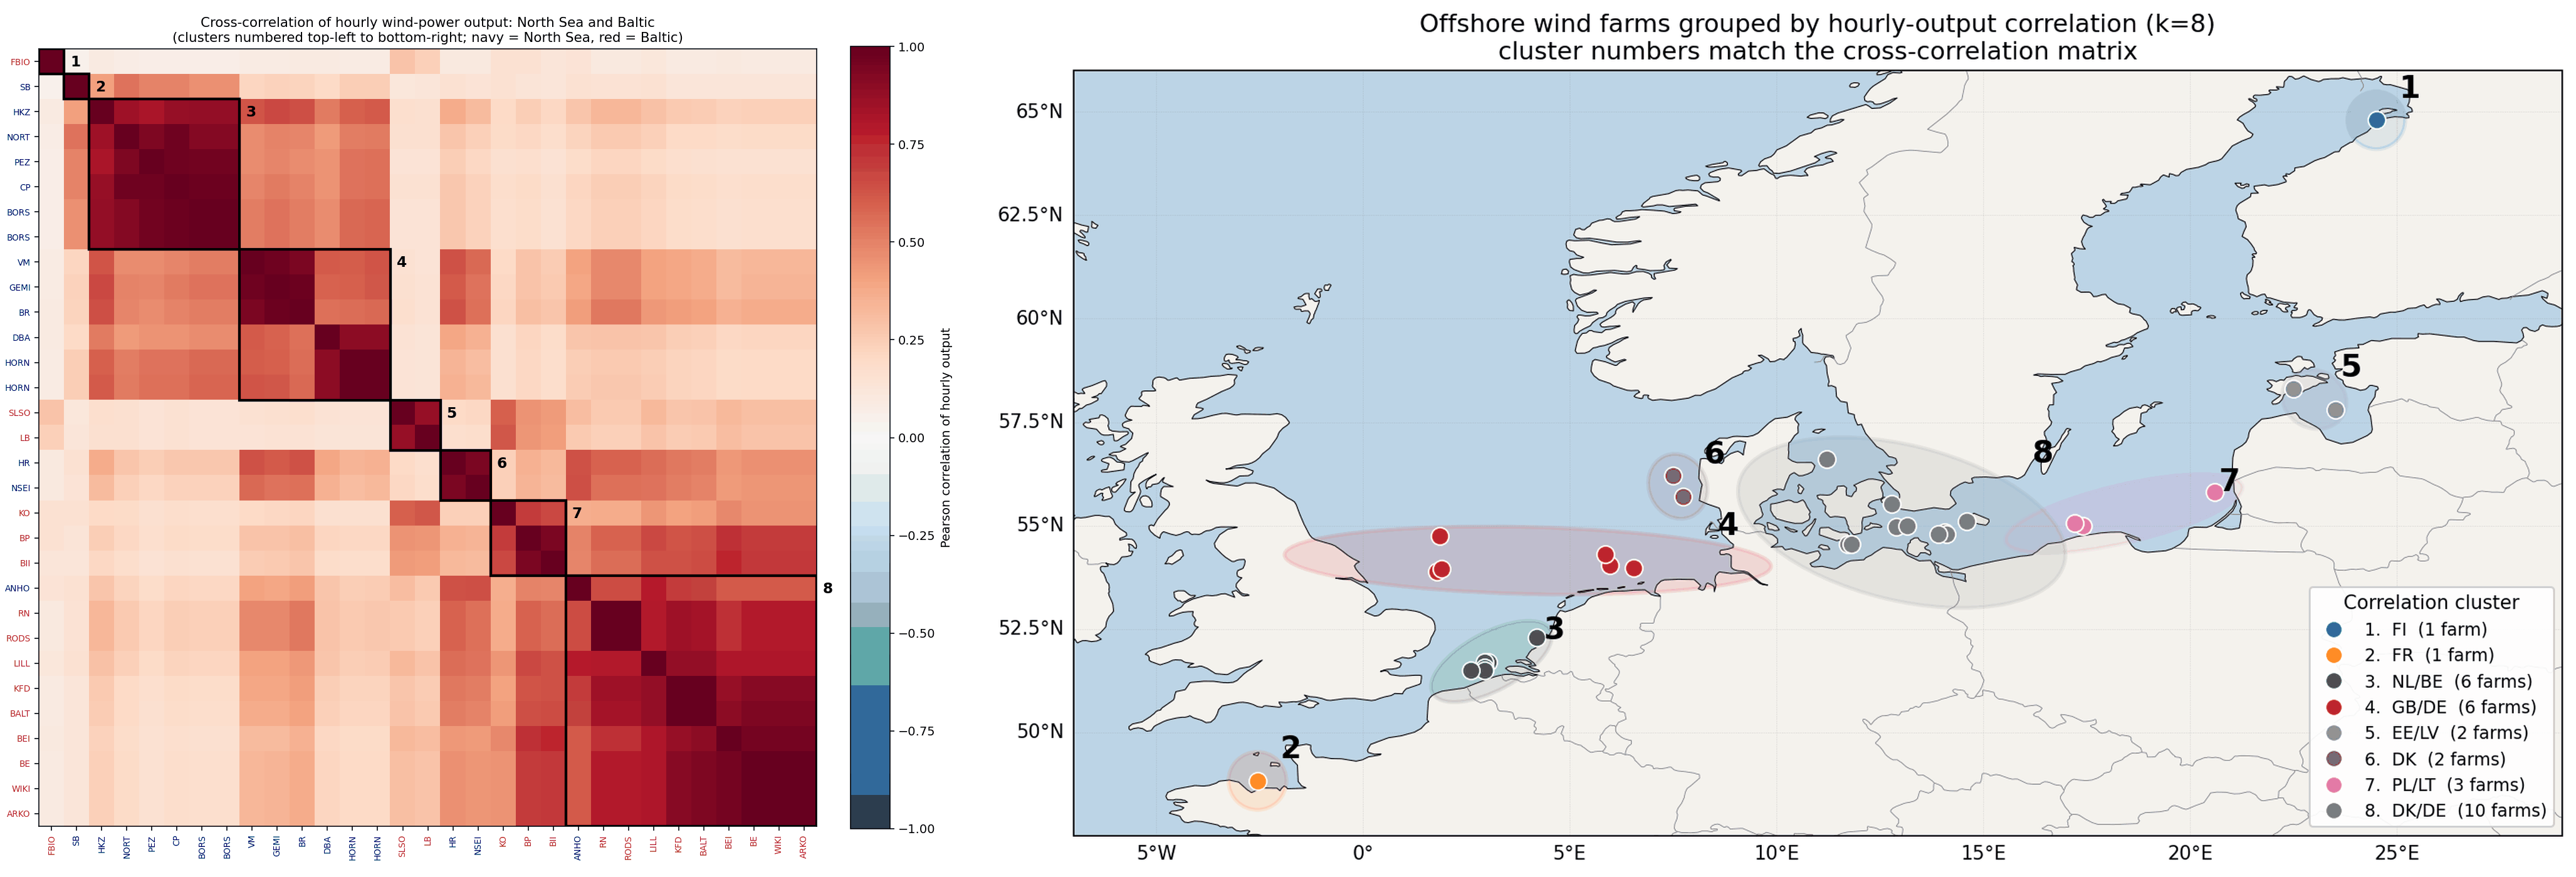
\includegraphics[width=0.80\textwidth]{fig_clusters_matrix_map}
    \caption{The 30-node clustering of the study region, showing which physical
    buses are aggregated into each model node. Copper-plating within a node is
    the limitation this resolution imposes, and the reason small well-connected
    zones carry the largest system-model bias.}
    \label{fig:clusters_map}
\end{figure}

\FloatBarrier
\subsection*{G.2 Measured capture value}

\begin{figure}[!htb]
    \centering
    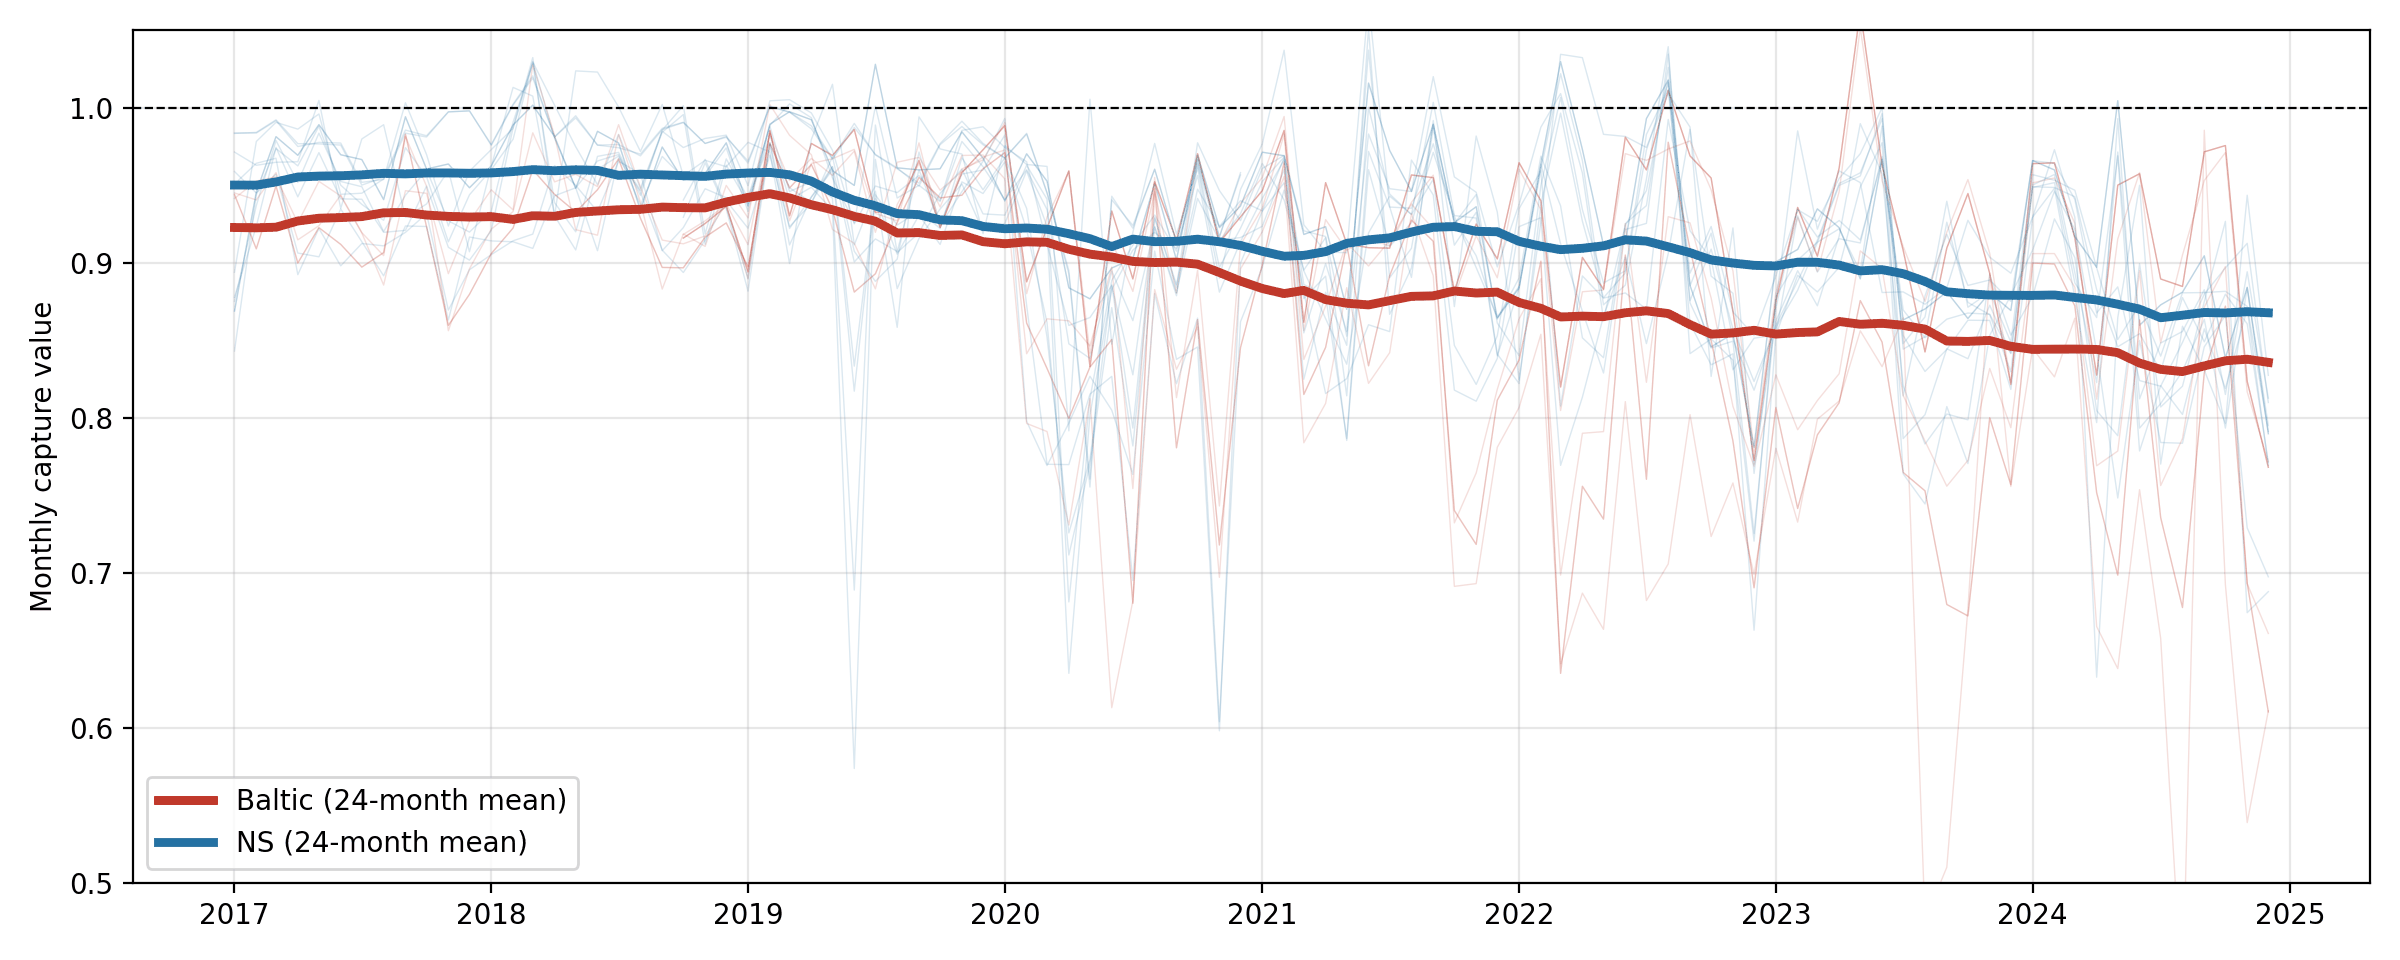
\includegraphics[width=0.88\textwidth]{fig_B_cv_history_basins}
    \caption{Eight years of measured capture value by basin, the full history
    behind the summary in Section~\ref{sec:eight_years}.}
    \label{fig:cv_history}
\end{figure}


\begin{figure}[!htb]
    \centering
    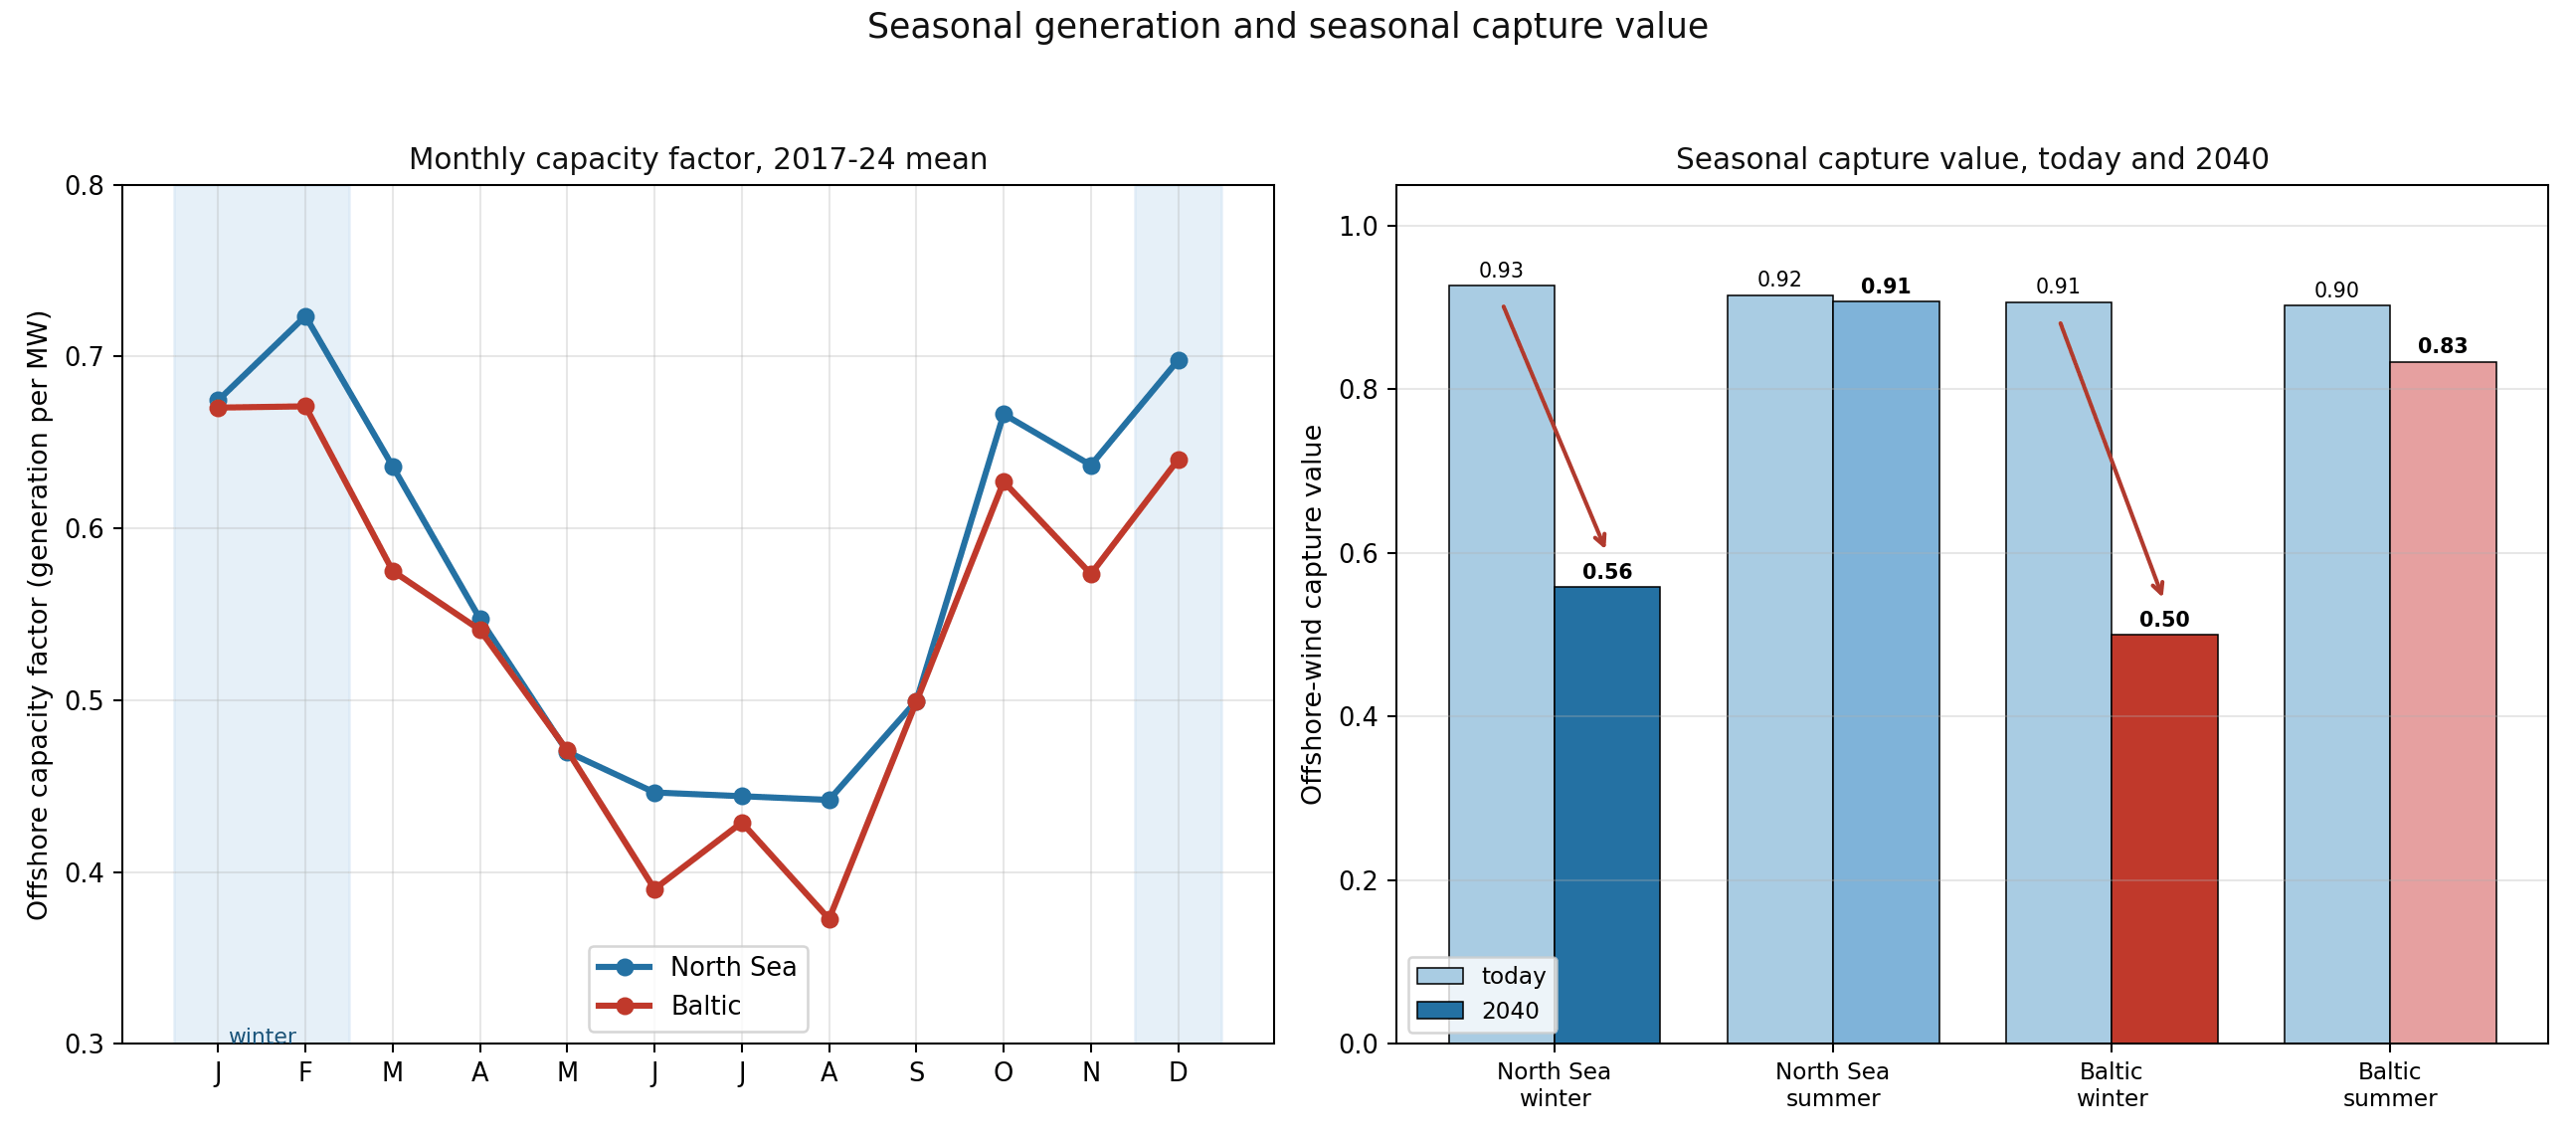
\includegraphics[width=0.88\textwidth]{fig_seasonal_generation}
    \caption{The seasonal generation profile and its interaction with capture
    value: output peaks in winter, which is also when the basins synchronise, so
    the largest volumes are sold into the most depressed hours.}
    \label{fig:seasonal_generation}
\end{figure}


\begin{figure}[!htb]
    \centering
    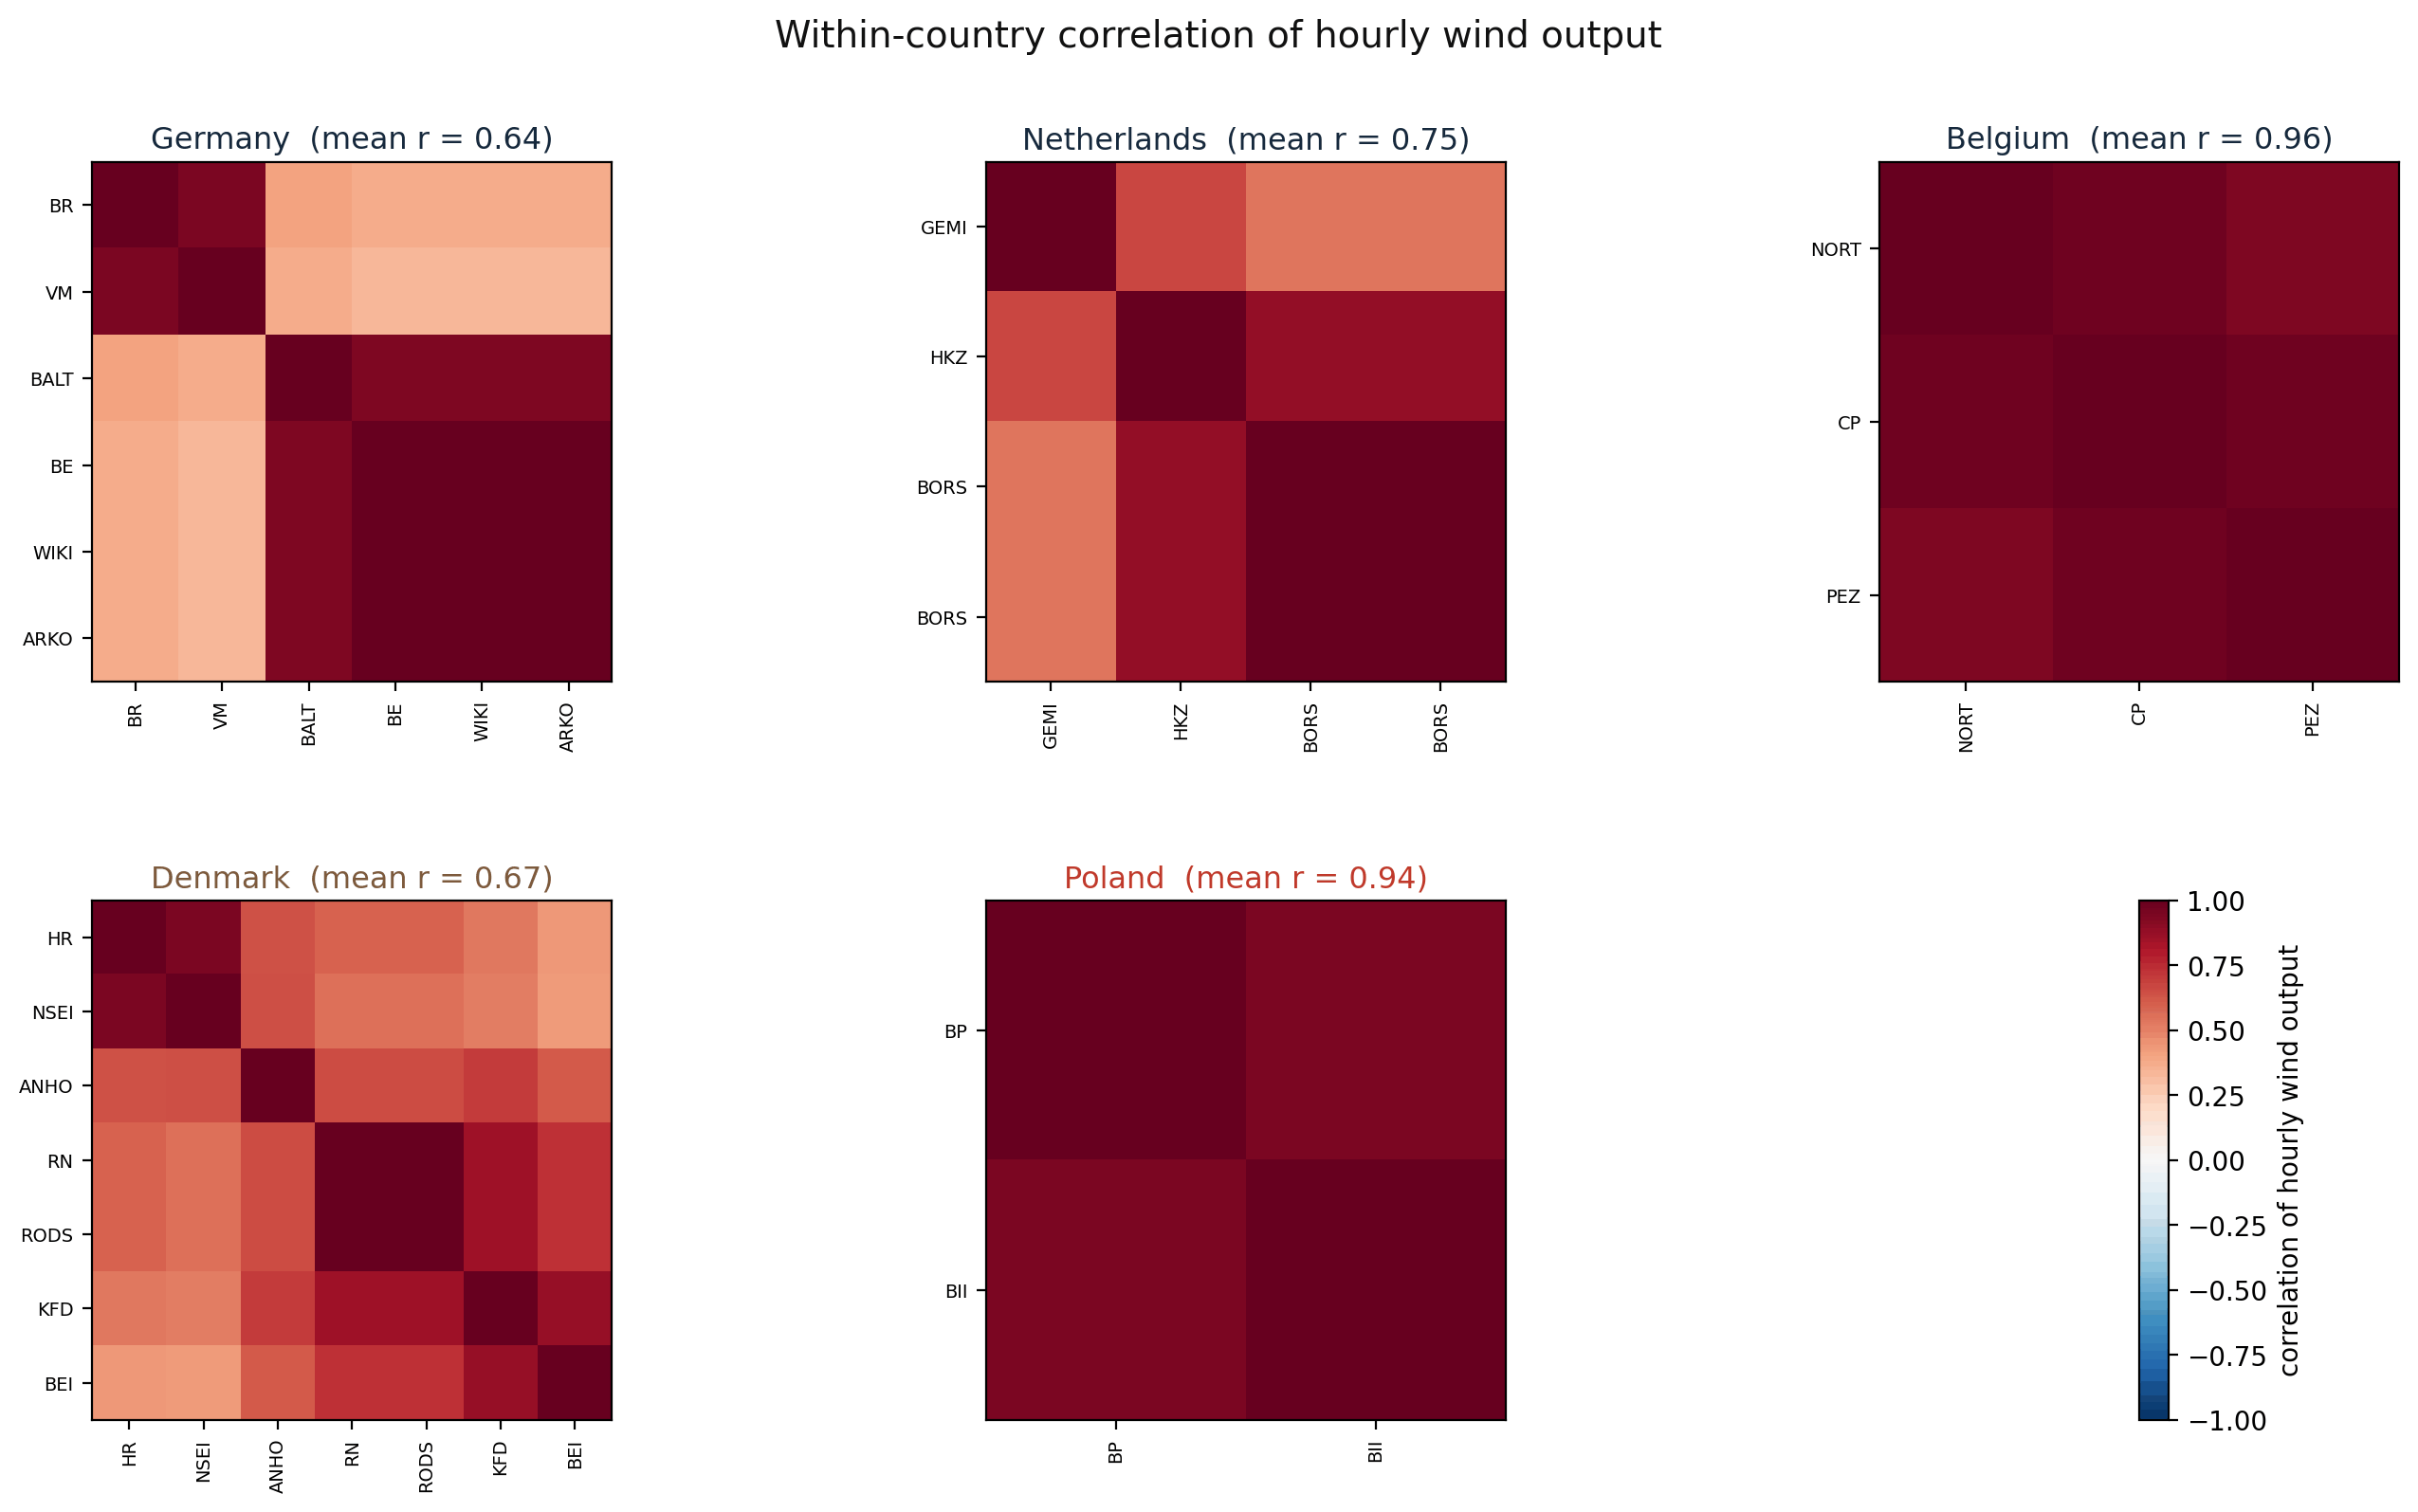
\includegraphics[width=0.88\textwidth]{fig_country_correlation}
    \caption{Within-country wind synchronicity matrices, the granular analogue
    of the basin correlation figure. Compact fleets blow nearly as one (Belgium
    0.96, Poland 0.94); spread fleets do not (Germany 0.64, Denmark 0.67).
    Germany splits into two blocks, its North Sea and Baltic farms, so the basin boundary dominates the national one.}
    \label{fig:country_correlation}
\end{figure}

\FloatBarrier
\subsection*{G.3 Within-Baltic convergence}



\begin{figure}[!htb]
    \centering
    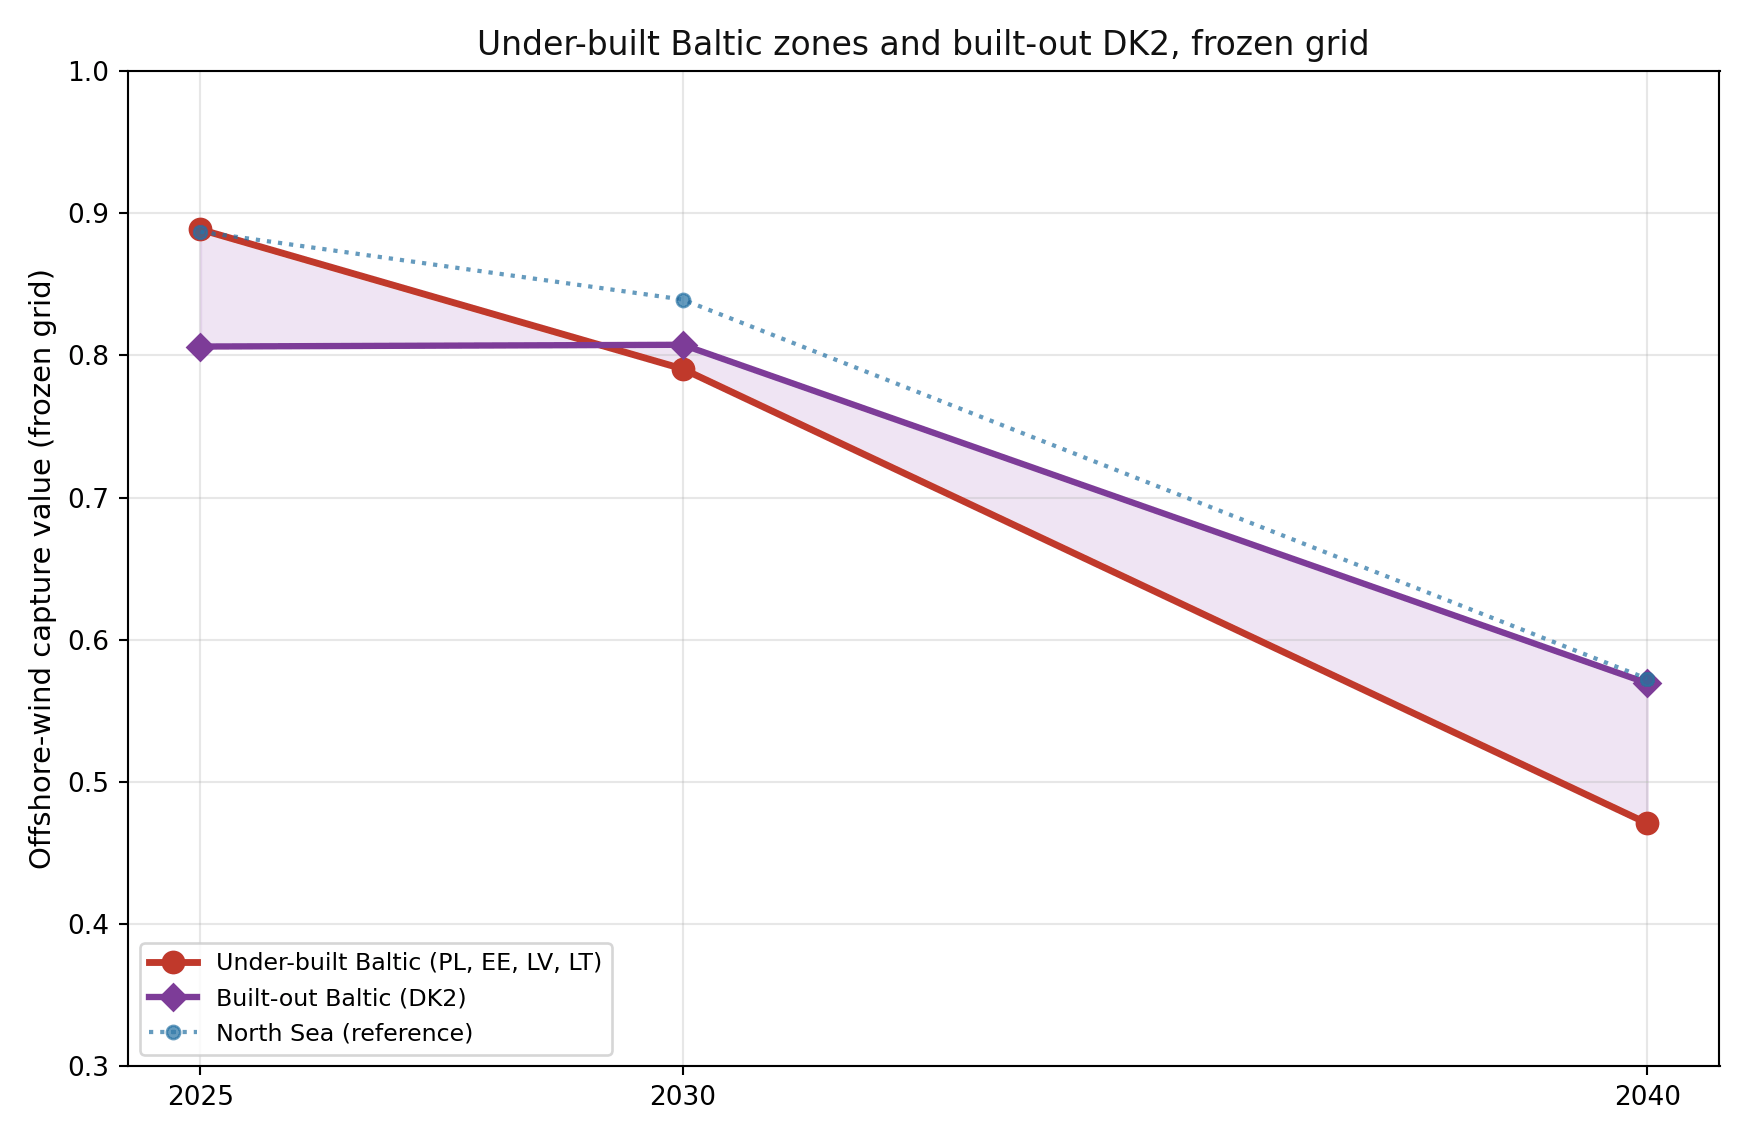
\includegraphics[width=0.88\textwidth]{fig_baltic_convergence}
    \caption{Convergence of the under-built Baltic zones onto the values already
    reached by the built-out DK2 and SE4, the space-for-time argument shown
    directly.}
    \label{fig:baltic_convergence}
\end{figure}




\FloatBarrier
\subsection*{G.4 Model diagnostics}



\begin{figure}[!htb]
    \centering
    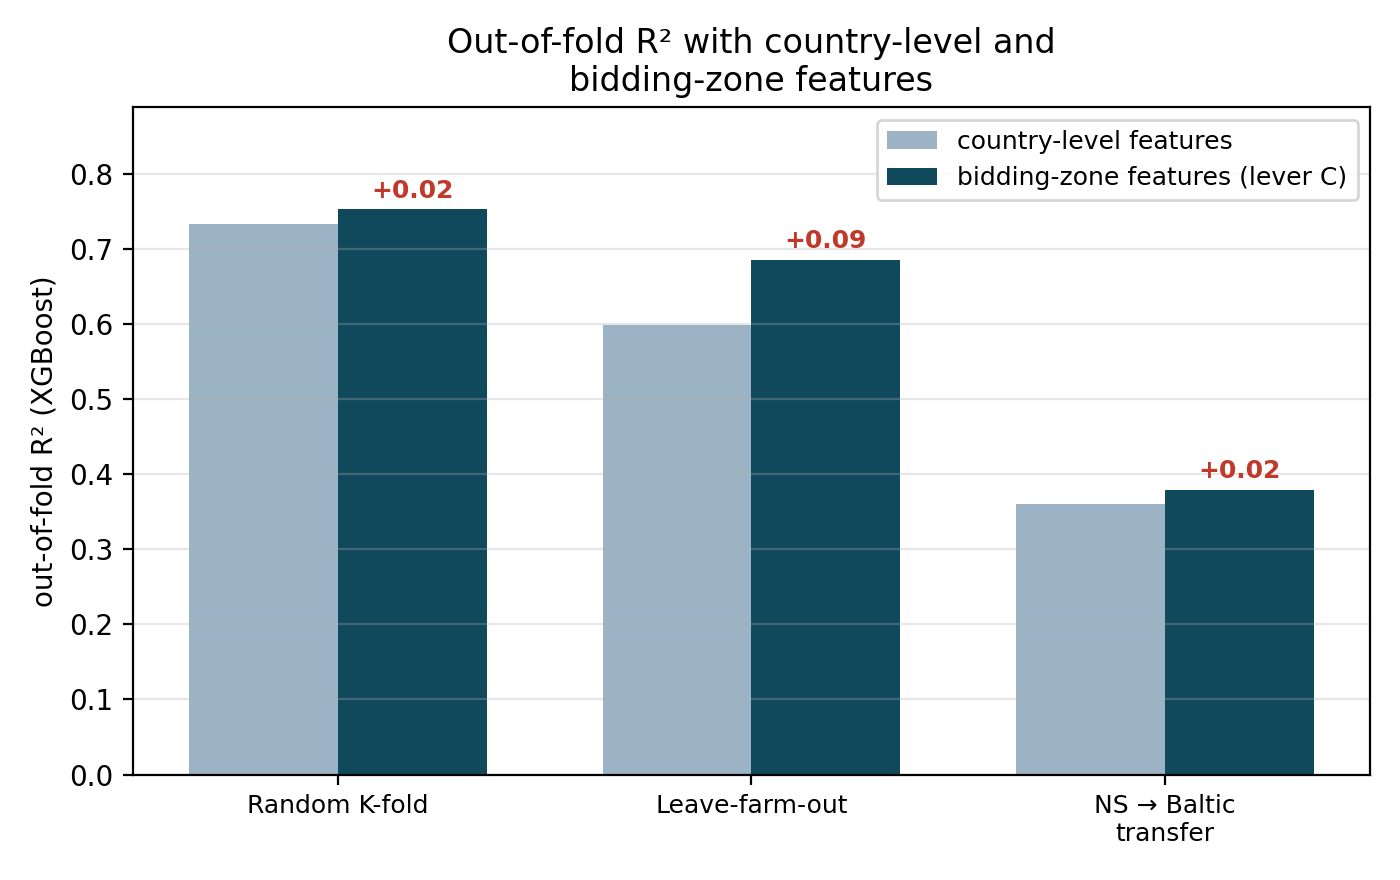
\includegraphics[width=0.7\textwidth]{fig_F_leverC_before_after}
    \caption{What bidding-zone resolution buys: out-of-sample $R^2$ before and
    after resolving features at the level prices form.}
    \label{fig:leverC}
\end{figure}

\begin{figure}[!htb]
    \centering
    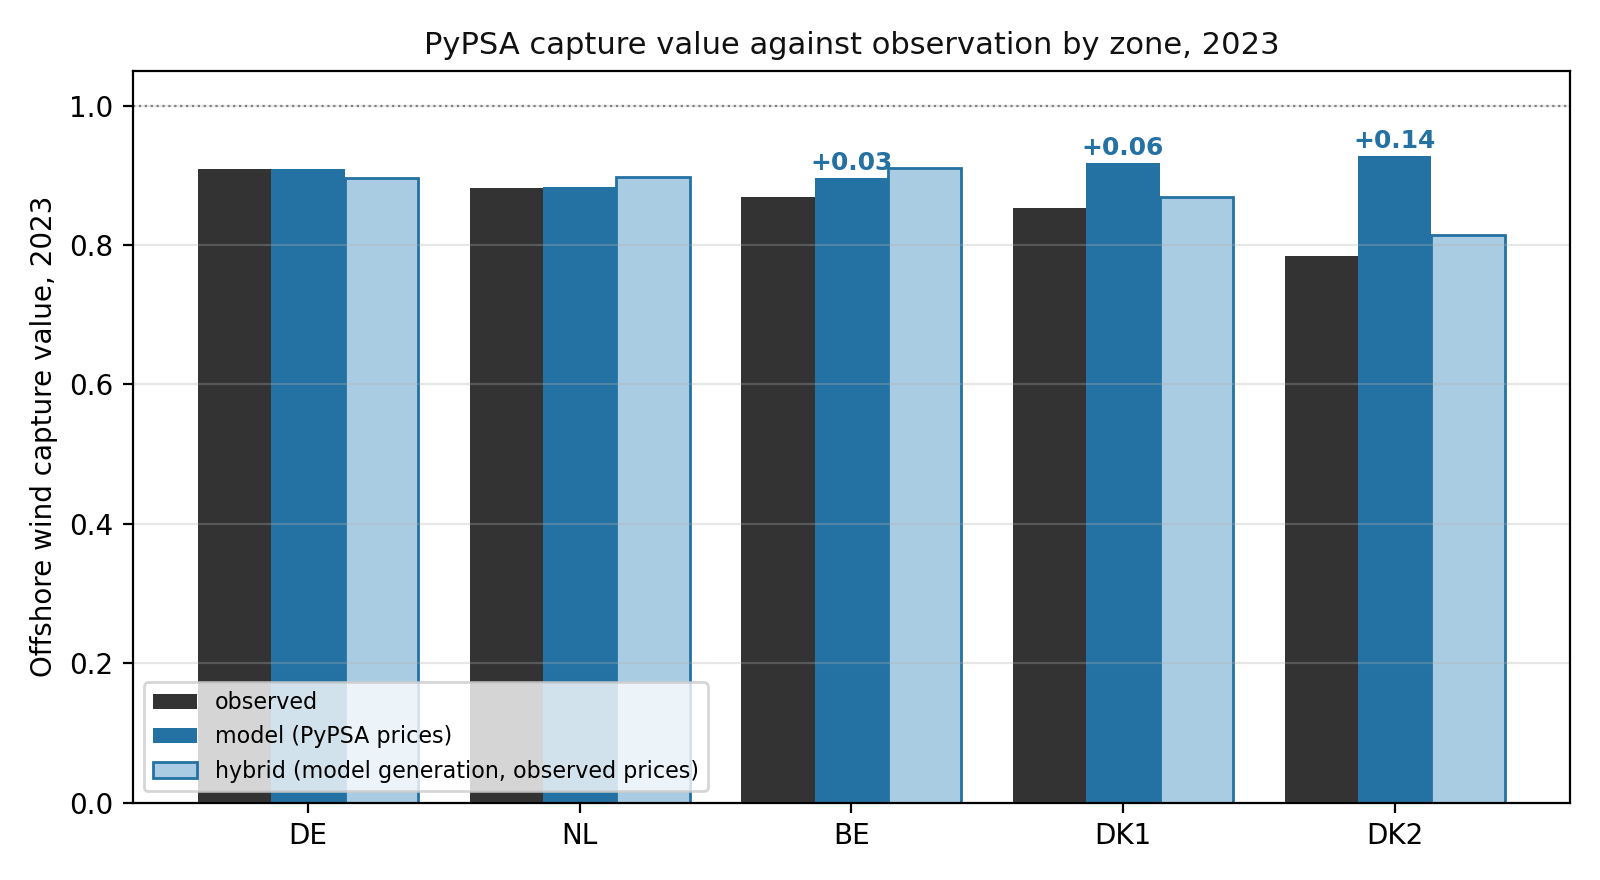
\includegraphics[width=0.85\textwidth]{fig_calibration_cv_2023}
    \caption{The system model's capture value, validated zone by zone for
    2023: observed, modelled, and the hybrid pairing modelled generation with
    observed prices. The model is near-exact in large zones and overstates
    capture value with congestion; the hybrid locates the error in the modelled prices and shows the modelled
    generation to be sound.}
    \label{fig:calibration_cv}
\end{figure}


\FloatBarrier
\subsection*{G.5 Robustness of the projection}

\begin{figure}[!htb]
    \centering
    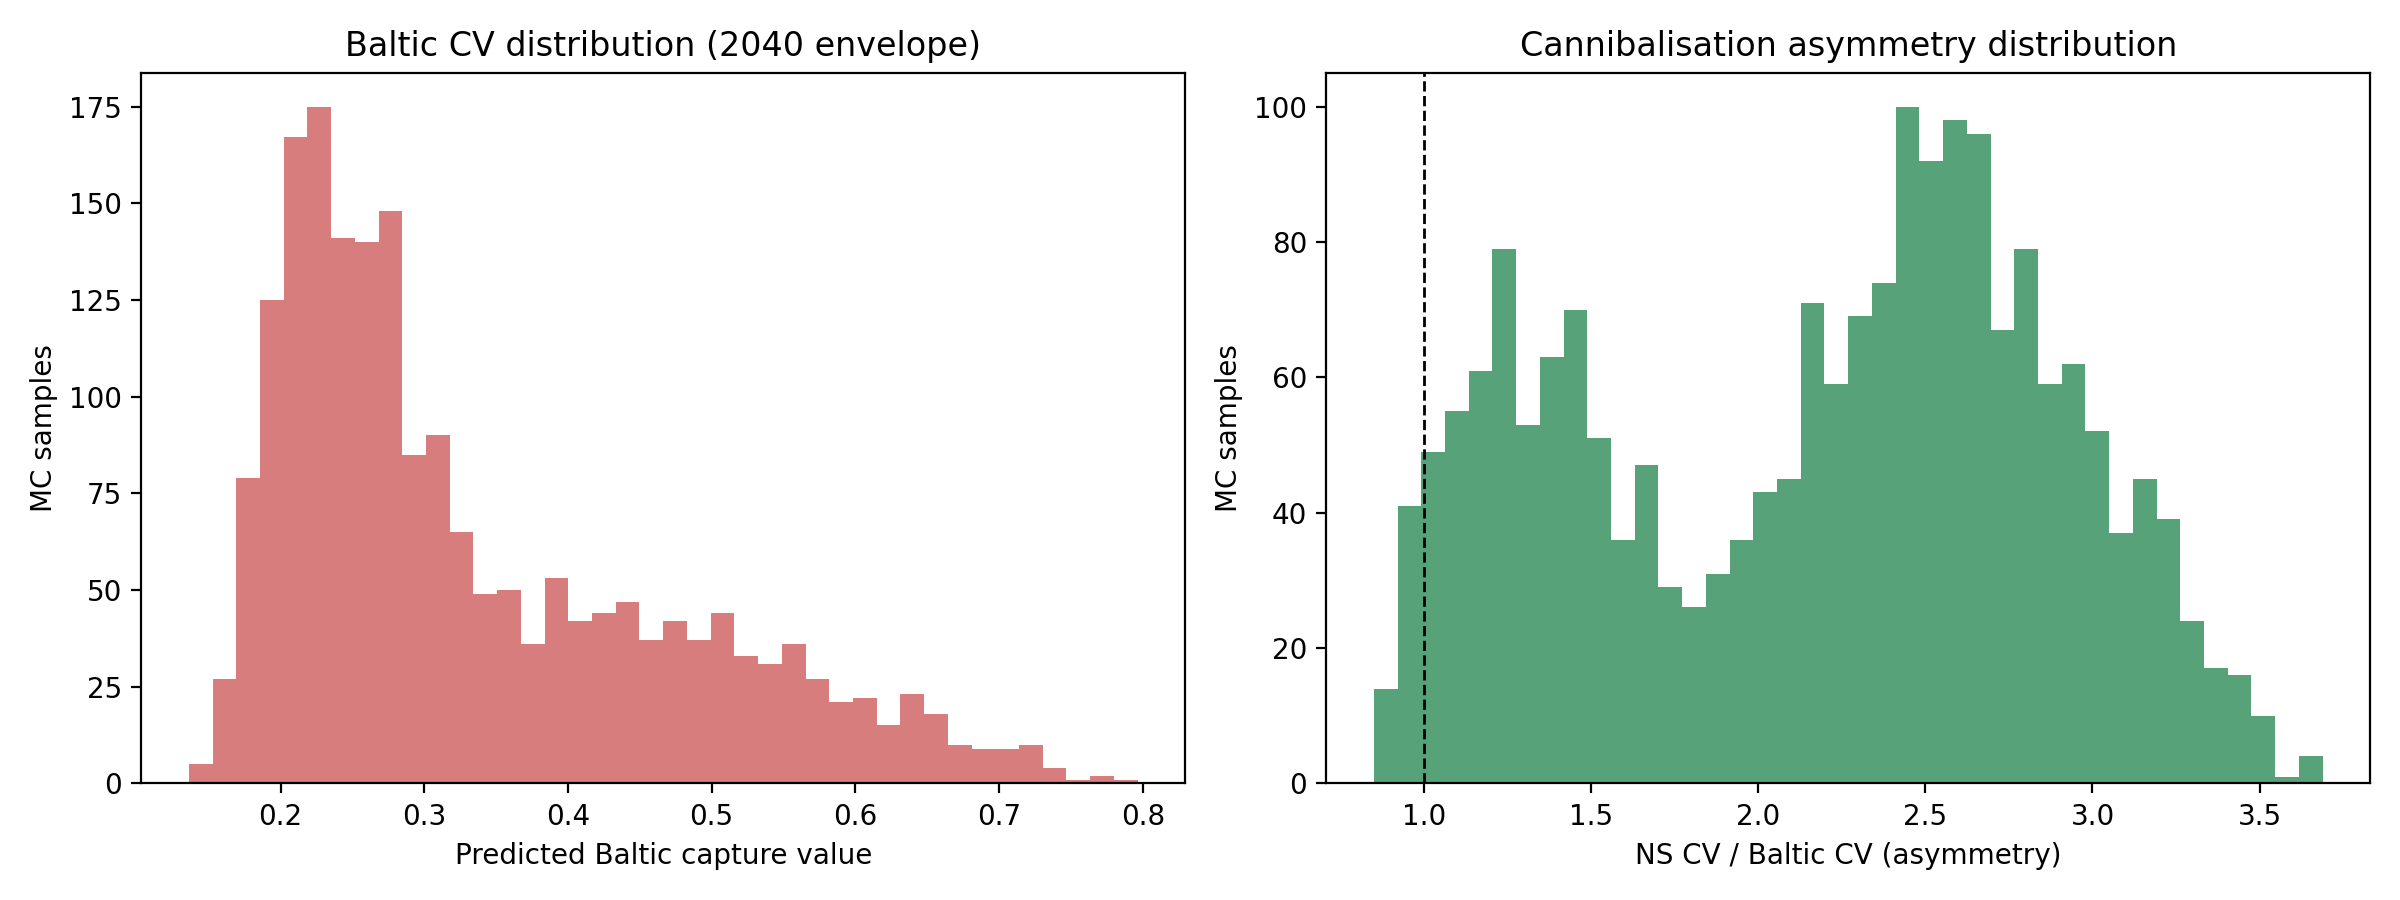
\includegraphics[width=0.85\textwidth]{fig_montecarlo}
    \caption{Monte-Carlo fans over the full input envelope (2,000 samples, inputs
    beyond TYNDP by design): Baltic capture value median 0.28, 90\,\% interval
    $[0.18, 0.62]$; North Sea to Baltic asymmetry median about 2.3$\times$. These figures describe the range of possibilities and give no single point
    result.}
    \label{fig:montecarlo}
\end{figure}

\begin{figure}[!htb]
    \centering
    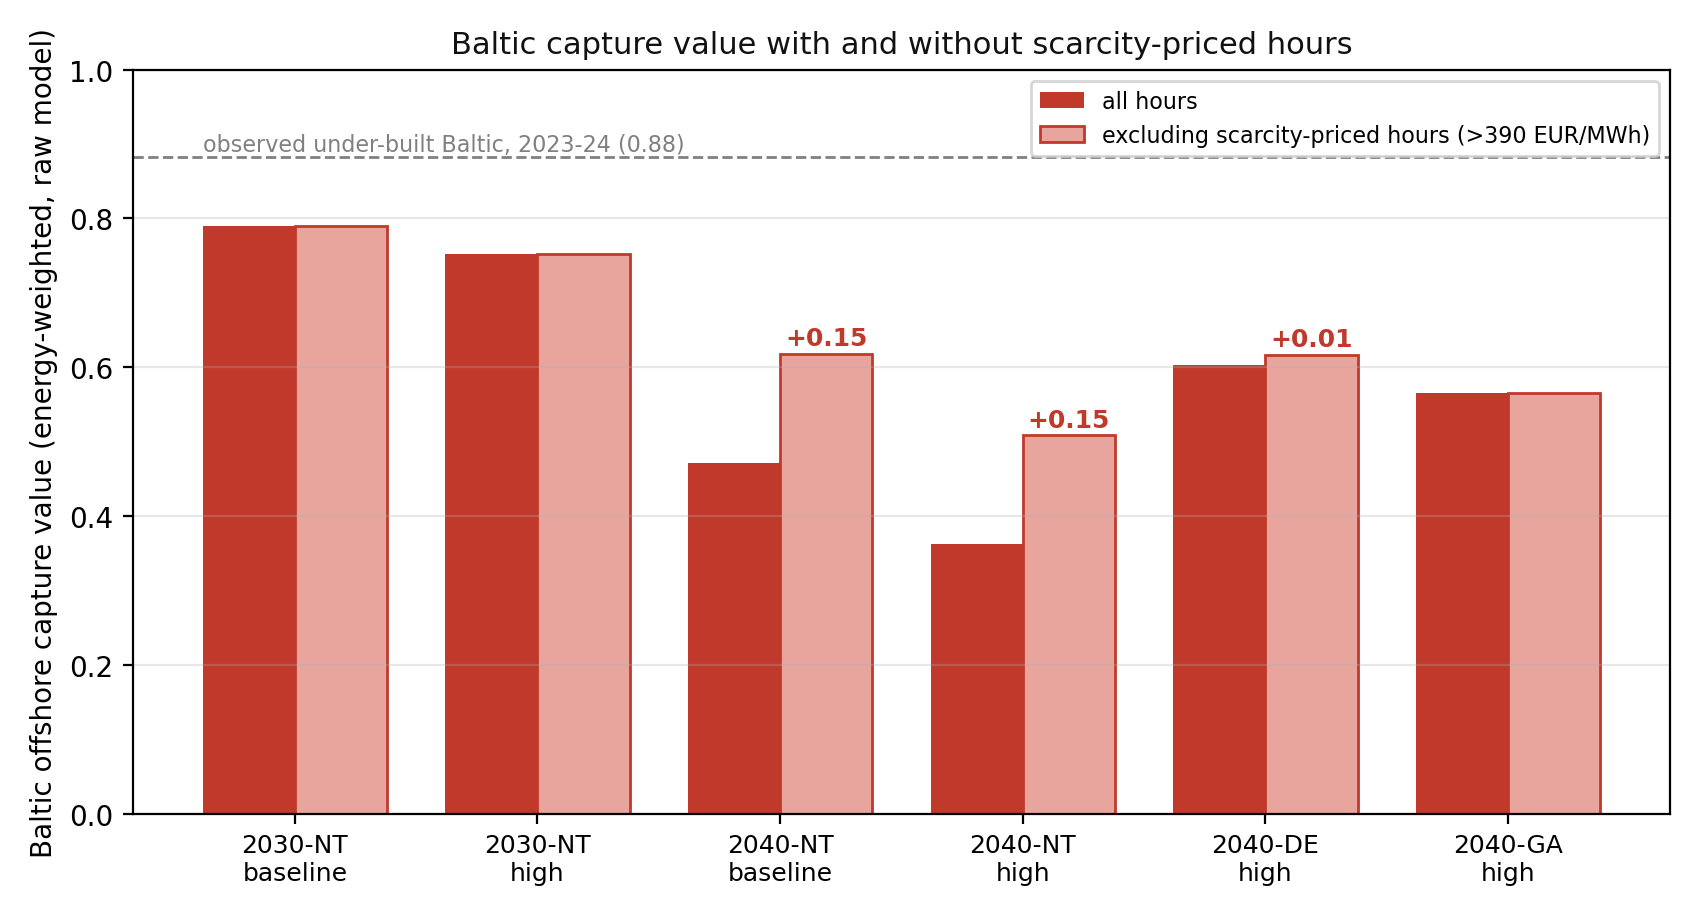
\includegraphics[width=0.9\textwidth]{fig_scarcity_bars}
    \caption{The fall survives the removal of scarcity-priced hours: Baltic capture value
    per scenario (uncorrected model), with and without scarcity-priced hours. The 2030 and clean 2040
    scenarios are scarcity-free; the NT 2040 scenarios carry a Polish adequacy
    component; severe erosion survives the exclusion in every case.}
    \label{fig:scarcity_bars}
\end{figure}


\begin{figure}[!htb]
    \centering
    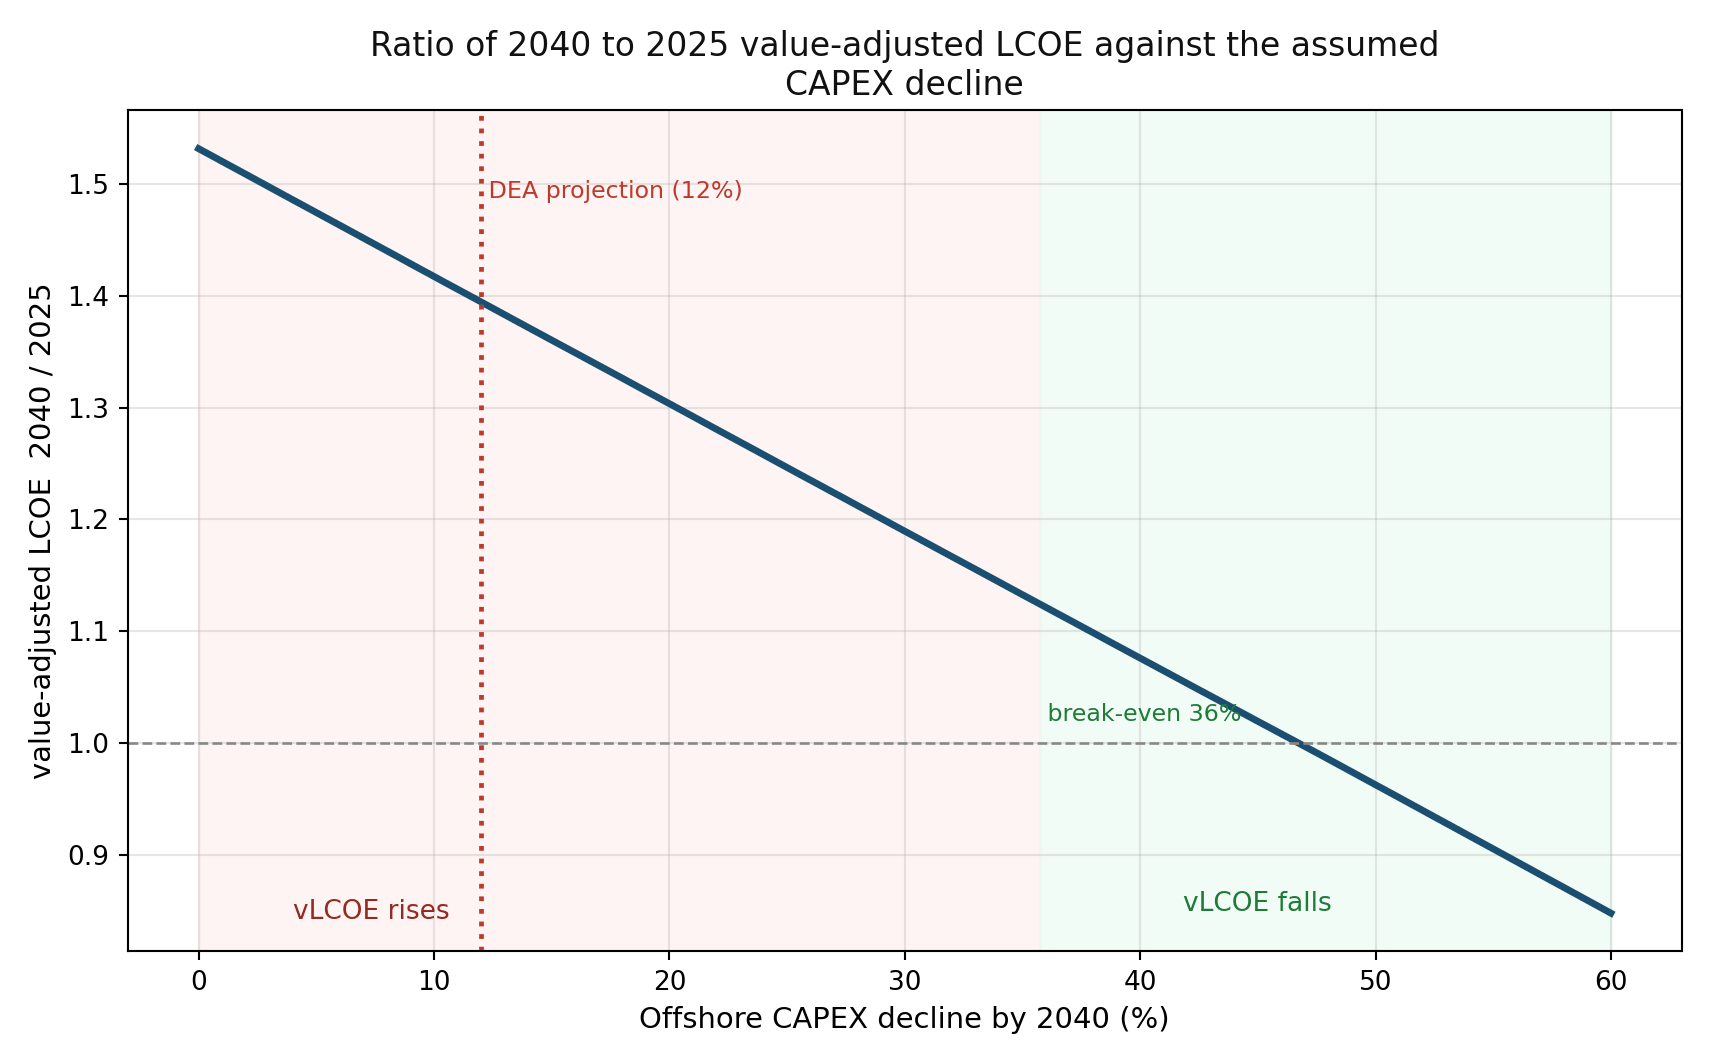
\includegraphics[width=0.82\textwidth]{fig_vlcoe_robustness}
    \caption{Robustness of the rising value-adjusted LCOE: the 2040-to-2025 ratio
    against the assumed offshore capital decline. It stays above one across the
    plausible range, and capital would have to fall about 36\%, against the
    database's 12\%, merely to hold the metric flat.}
    \label{fig:vlcoe_robust}
\end{figure}

\FloatBarrier
\subsection*{G.6 Mechanism: supporting detail}

\begin{figure}[!htb]
    \centering
    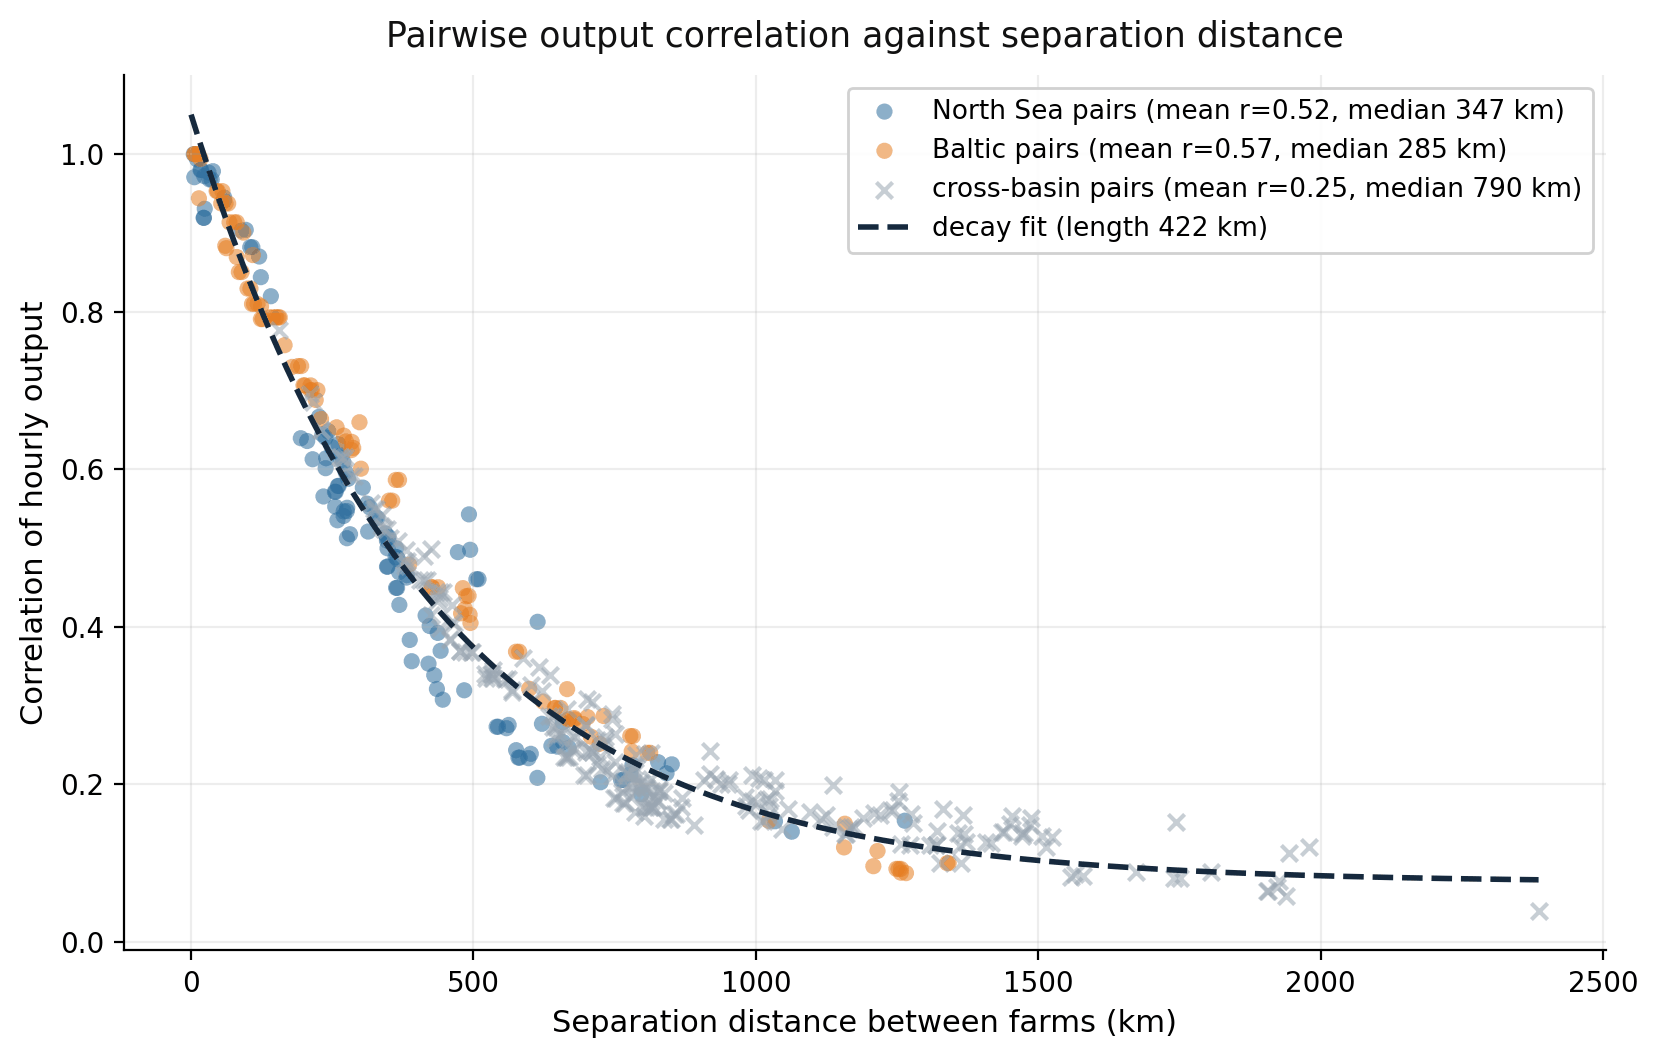
\includegraphics[width=0.78\textwidth]{fig_corr_vs_distance}
    \caption{Pairwise correlation of hourly wind output against separation
    distance, every farm pair, 2017 to 2024. All pairs follow one decay curve
    (fitted length 422~km); the Baltic pairs (mean 0.57) sit slightly above the
    North Sea pairs (mean 0.52), with a shorter typical separation (median 285
    against 347~km), while cross-basin pairs (mean 0.25) lie far out along the curve.}
    \label{fig:corr_distance}
\end{figure}

\begin{figure}[!htb]
    \centering
    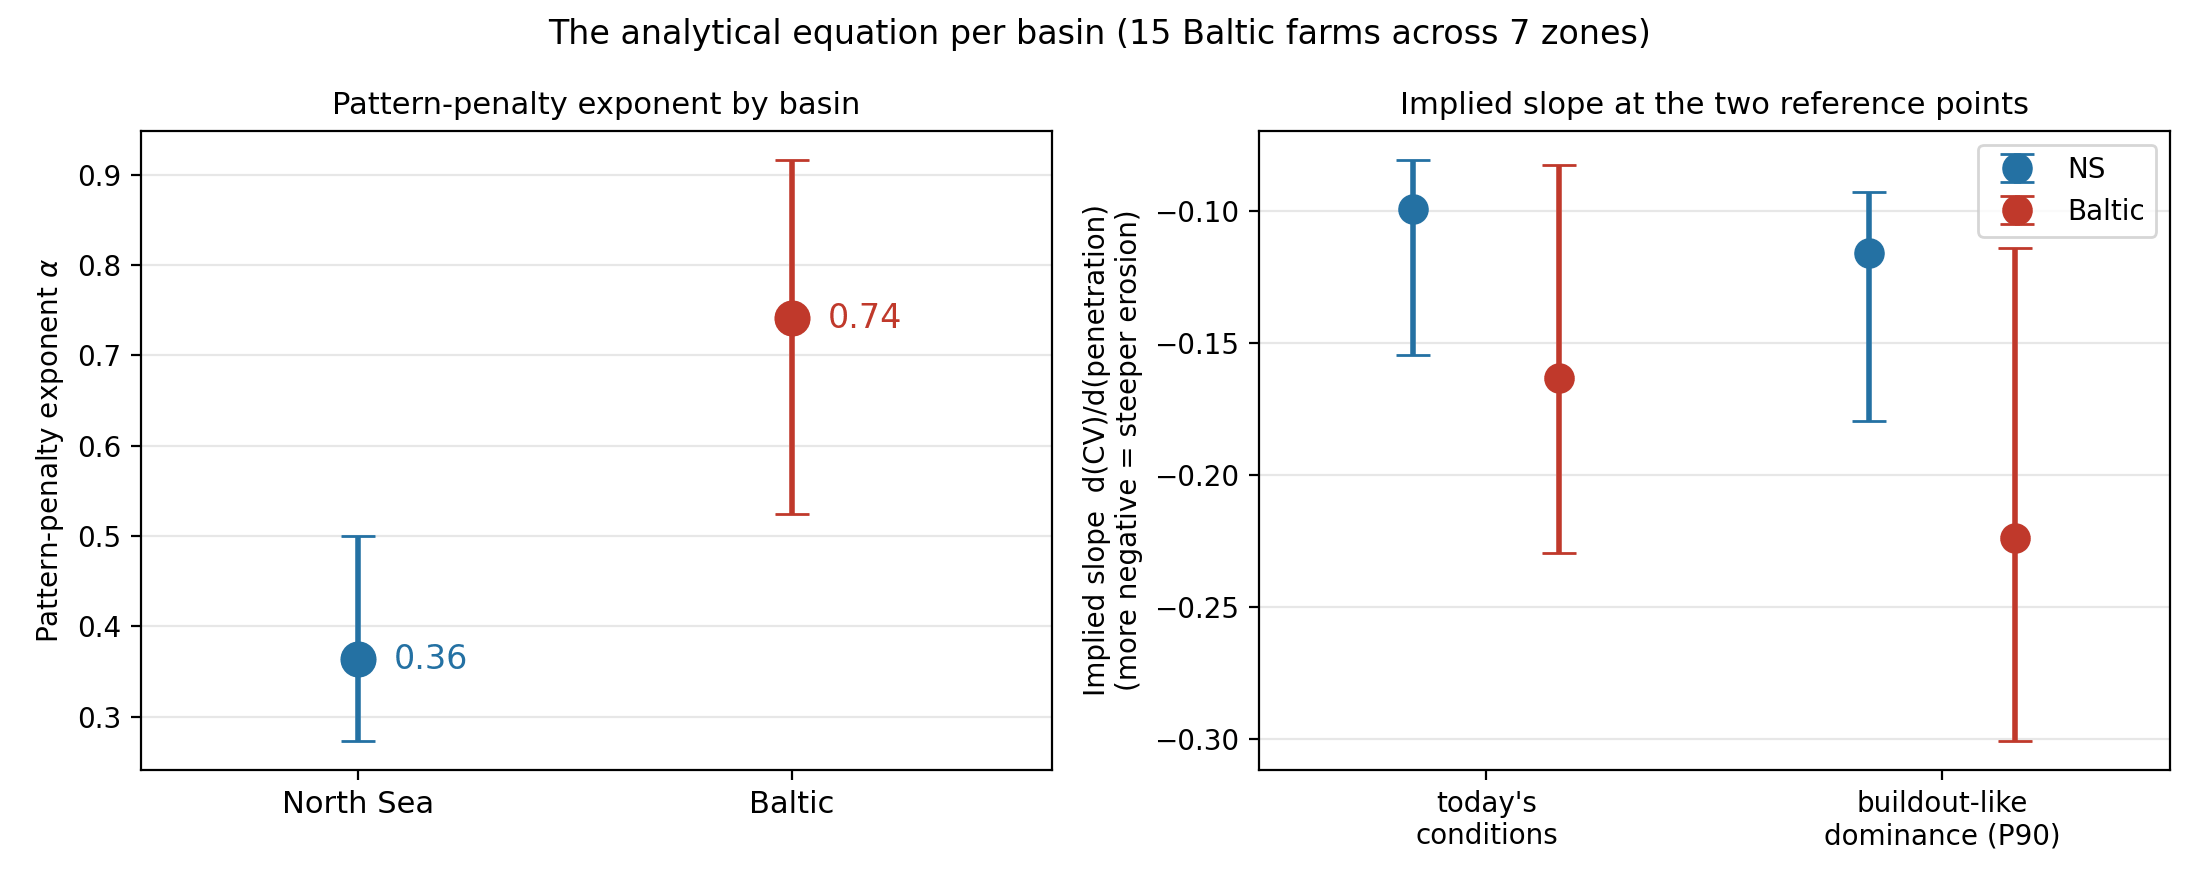
\includegraphics[width=0.9\textwidth]{fig_constants_comparison}
    \caption{The analytical equation refit per basin on the seven-zone panel
    (fifteen Baltic farms). Left: the pattern-penalty exponent is steeper in the
    Baltic (0.74 versus 0.37). Right: the implied slope of capture value against
    penetration is about 1.6 times steeper for the Baltic today and 1.9 times at
    buildout-like dominance. Whiskers are farm-block bootstrap 90\,\% intervals;
    the comparison is directional on a small panel.}
    \label{fig:constants}
\end{figure}

